%%%%%%%%%%%%%%%%%%%%%%%%%%%%%%%%%%%%%%%%%
% Imperial College London Presentation
% LaTeX Template
% Version 1.0 (April 16, 2024)
%
% This template was created by:
% Vel (enquiries@latextypesetting.com)
% LaTeXTypesetting.com
%
%!TEX program = xelatex
% Note: this template must be compiled with XeLaTeX rather than PDFLaTeX
% due to the custom fonts used. The line above should ensure this happens
% automatically, but if it doesn't, your LaTeX editor should have a simple toggle
% to switch to using XeLaTeX.
%
% © Imperial College London, 2024. This template, including logo and fonts, is 
% for use of Imperial staff and students only for university business. All rights 
% reserved to the copyright owners.
%
%%%%%%%%%%%%%%%%%%%%%%%%%%%%%%%%%%%%%%%%%

%----------------------------------------------------------------------------------------
%	CLASS, PACKAGES AND OTHER DOCUMENT CONFIGURATIONS
%----------------------------------------------------------------------------------------

\documentclass[
	aspectratio=169, % Uncomment to use an aspect ratio of 16:9 (160 mm by 90 mm)
	%aspectratio=43, % Uncomment to use an aspect ratio of 4:3 (128mm by 96mm)
	t, % Top align all slide content by default
	onlytextwidth, % Typeset content in columns at text width
	10pt, % Default font size, use 10pt for the 16:9 aspect ratio and 8pt for the 4:3 aspect ratio
]{beamer}

\usepackage{../ImperialTheme/beamerthemeImperial} % Use the Imperial theme

\def\imagefolder{../ImperialTheme/Images/}
%----------------------------------------------------------------------------------------
%	IMPERIAL BEAMER THEME USAGE NOTES
%----------------------------------------------------------------------------------------

% This theme features several predefined Imperial colors which can be used for text and slide backgrounds:
% ICLBlue - Most common slide background color and text color to use (on light backgrounds)
% ICLDarkBlue - Optional darker blue color for slide backgrounds and text
% ICLCream - Accessible background color for use on slide backgrounds
% ICLLightGrey - Accessible background color for use on slide backgrounds

% You can choose to use a 16:9 aspect ratio (default) or a 4:3 aspect ratio by uncommenting the relevant line in the \documentclass specifications above. Note that if you switch between the 2 aspect ratios, you will likely need to adjust how your images are included in the presentation. Usually for a 16:9 aspect ratio, images will be included as width=\paperwidth, but for a 4:3 aspect ratio it's recommended to use height=\paperheight instead.

%----------------------------------------------------------------------------------------
%	PRESENTATION INFORMATION
%----------------------------------------------------------------------------------------

\title{Presentation Title} % Presentation title to appear on the title slide and left footers

\subtitle{Subheading} % Presentation subtitle to appear on the title slide

\author{Author Name} % Author name(s) to appear on the title slide

\date{DD/MM/YYYY} % Presentation date to appear on the title slide and right footers

%----------------------------------------------------------------------------------------

\begin{document}

%----------------------------------------------------------------------------------------
%	TITLE SLIDES
%----------------------------------------------------------------------------------------

% Select one of the 3 title slide types below and remove or comment out the others

%------------------------------------------------

% Blue background title slide example

\begingroup
	\setbeamercolor{background canvas}{bg=ICLBlue} % Slide background color
	\setbeamercolor{title page title}{fg=white} % Title text color
	\setbeamercolor{title page subtitle}{fg=white} % Subtitle text color
	\setbeamercolor{author}{fg=white} % Author(s) text color
	\setbeamercolor{date}{fg=white} % Date text color
	\setbeamertemplate{title page}[logo]{\imagefolder/ICL_Logo_White.pdf} % Imperial logo color, use 'ICL_Logo_White.pdf' for white and 'ICL_Logo_Blue.pdf' for blue
	\frame[plain, s]{\titlepage} % Output the title page with no footer ('plain') and vertically distributed text ('s')
\endgroup

%------------------------------------------------

% White background title slide example

\begingroup
	\setbeamercolor{title page title}{fg=ICLBlue} % Title text color
	\setbeamercolor{title page subtitle}{fg=ICLBlue} % Subtitle text color
	\setbeamercolor{author}{fg=ICLBlue} % Author(s) text color
	\setbeamercolor{date}{fg=ICLBlue} % Date text color
	\setbeamertemplate{title page}[logo]{\imagefolder/ICL_Logo_Blue.pdf} % Imperial logo color, use 'ICL_Logo_White.pdf' for white and 'ICL_Logo_Blue.pdf' for blue
	\frame[plain, s]{\titlepage} % Output the title page with no footer ('plain') and vertically distributed text ('s')
\endgroup

%------------------------------------------------

% Cream background title slide example

\begingroup
	\setbeamercolor{background canvas}{bg=ICLCream} % Slide background color
	\setbeamercolor{title page title}{fg=ICLBlue} % Title text color
	\setbeamercolor{title page subtitle}{fg=ICLBlue} % Subtitle text color
	\setbeamercolor{author}{fg=ICLBlue} % Author(s) text color
	\setbeamercolor{date}{fg=ICLBlue} % Date text color
	\setbeamertemplate{title page}[logo]{\imagefolder/ICL_Logo_Blue.pdf} % Imperial logo color, use 'ICL_Logo_White.pdf' for white and 'ICL_Logo_Blue.pdf' for blue
	\frame[plain, s]{\titlepage} % Output the title page with no footer ('plain') and vertically distributed text ('s')
\endgroup

%------------------------------------------------

% Light grey background title slide example

\begingroup
	\setbeamercolor{background canvas}{bg=ICLLightGrey} % Slide background color
	\setbeamercolor{title page title}{fg=ICLBlue} % Title text color
	\setbeamercolor{title page subtitle}{fg=ICLBlue} % Subtitle text color
	\setbeamercolor{author}{fg=ICLBlue} % Author(s) text color
	\setbeamercolor{date}{fg=ICLBlue} % Date text color
	\setbeamertemplate{title page}[logo]{\imagefolder/ICL_Logo_Blue.pdf} % Imperial logo color, use 'ICL_Logo_White.pdf' for white and 'ICL_Logo_Blue.pdf' for blue
	\frame[plain, s]{\titlepage} % Output the title page with no footer ('plain') and vertically distributed text ('s')
\endgroup

%------------------------------------------------

% Full page image background title slide example

\begingroup
	\setbeamertemplate{background}{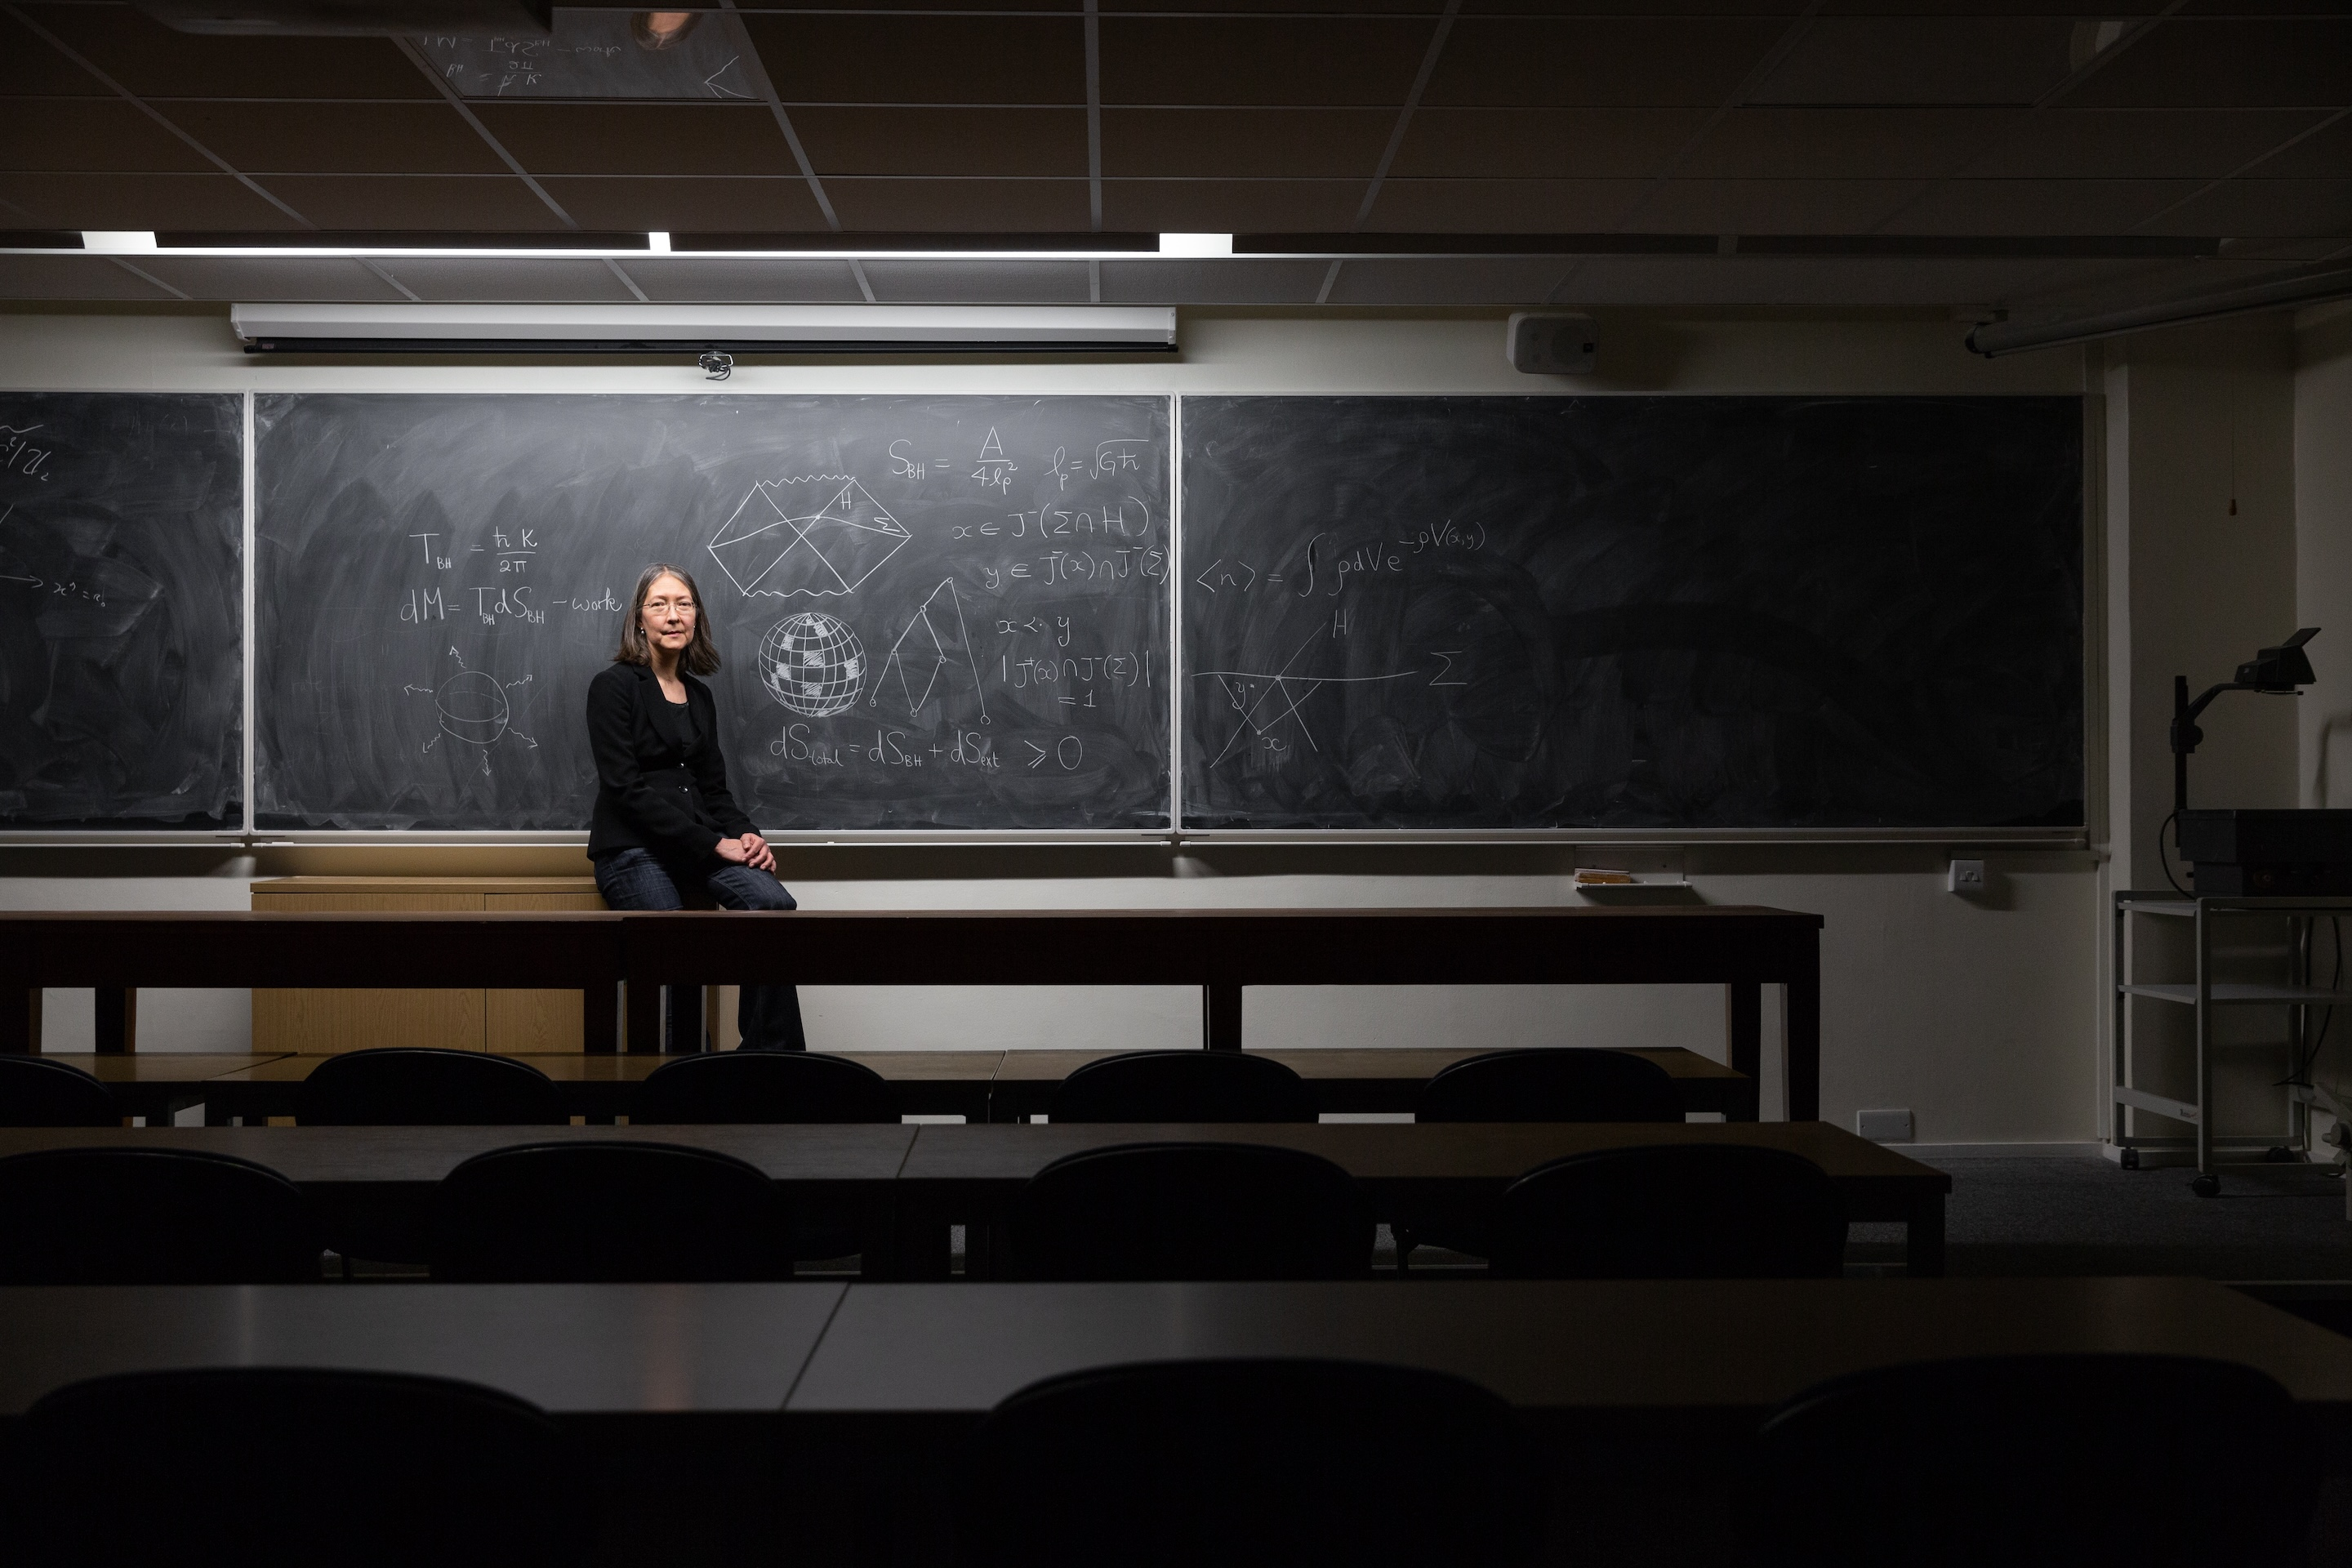
\includegraphics[width=\paperwidth]{\imagefolder/190211_dowker_fay_001.jpg}} % Slide background image
	\setbeamercolor{title page title}{fg=white} % Title text color
	\setbeamercolor{title page subtitle}{fg=white} % Subtitle text color
	\setbeamercolor{author}{fg=white} % Author(s) text color
	\setbeamercolor{date}{fg=white} % Date text color
	\setbeamertemplate{title page}[logo]{\imagefolder/ICL_Logo_White.pdf} % Imperial logo color, use 'ICL_Logo_White.pdf' for white and 'ICL_Logo_Blue.pdf' for blue
	\frame[plain, s]{\titlepage} % Output the title page with no footer ('plain') and vertically distributed text ('s')
\endgroup

%----------------------------------------------------------------------------------------
%	AGENDA SLIDES
%----------------------------------------------------------------------------------------

% White agenda slide

\begingroup
	\setbeamercolor{normal text}{fg=ICLBlue}\usebeamercolor[fg]{normal text} % Slide text color
	
	\begin{frame}
		\begin{columns}[T] % [T] ensures correct vertical alignment
			\begin{column}{0.48\linewidth} % Left column
				\HUGE\textbf{Agenda}
			\end{column}
			\begin{column}{0.48\linewidth} % Right column
				\textbf{01}\tabto{0.125\linewidth} Who we are\\ % Use \tabto{<length>} to add a fixed horizontal whitespace
				\textbf{02}\tabto{0.125\linewidth} What we do\\
				\textbf{03}\tabto{0.125\linewidth} Our process\\
				\textbf{04}\tabto{0.125\linewidth} Our services\\
				\textbf{05}\tabto{0.125\linewidth} Who we do it for\\
				\textbf{06}\tabto{0.125\linewidth} Lorem ipsum\\
				\textbf{07}\tabto{0.125\linewidth} Dolor amet\\
				\textbf{08}\tabto{0.125\linewidth} Oluptibus autud
				
				\textbf{Lorem ipsum dolor sit amet, consectetur adipiscing elit. Praesent porttitor arcu luctus, imperdiet urna iaculis, mattis eros.}
			\end{column}
		\end{columns}
	\end{frame}
\endgroup

%------------------------------------------------

% Blue agenda slide

\begingroup
	\setbeamercolor{background canvas}{bg=ICLBlue} % Slide background color
	\setbeamercolor{normal text}{fg=white}\usebeamercolor[fg]{normal text} % Slide text color
	\setbeamercolor{page number in head/foot}{fg=white} % Footer text color
	
	\begin{frame}
		\begin{columns}[T] % [T] ensures correct vertical alignment
			\begin{column}{0.48\linewidth} % Left column
				\HUGE\textbf{Agenda}
			\end{column}
			\begin{column}{0.48\linewidth} % Right column
				\textbf{01}\tabto{0.125\linewidth} Who we are\\ % Use \tabto{<length>} to add a fixed horizontal whitespace
				\textbf{02}\tabto{0.125\linewidth} What we do\\
				\textbf{03}\tabto{0.125\linewidth} Our process\\
				\textbf{04}\tabto{0.125\linewidth} Our services\\
				\textbf{05}\tabto{0.125\linewidth} Who we do it for\\
				\textbf{06}\tabto{0.125\linewidth} Lorem ipsum\\
				\textbf{07}\tabto{0.125\linewidth} Dolor amet\\
				\textbf{08}\tabto{0.125\linewidth} Oluptibus autud
				
				\textbf{Lorem ipsum dolor sit amet, consectetur adipiscing elit. Praesent porttitor arcu luctus, imperdiet urna iaculis, mattis eros.}
			\end{column}
		\end{columns}
	\end{frame}
\endgroup

%----------------------------------------------------------------------------------------
%	PRESENTATION BODY SLIDE EXAMPLES
%----------------------------------------------------------------------------------------

\begin{frame}
	\frametitle{Slide Title}
	\framesubtitle{Optional Slide Subtitle}
	
	\begin{adjustwidth}{0cm}{0.35\textwidth} % The first parameter is the left margin indentation and the second is the right margin indentation
		Sed et mincipidem am fugia venihitem aut utatem invellupis dolore voluptatiate verior mo dolendi squatur?

		Ab illate sitate explibus reiundusam, voluptur sim idebit, omnis dero quas adio quatur?

		Pa cumquat ute nos exero magnime officatem. Luptia voluptatur aut acia comnist qui beatusam, omniatecae iur alit, cus debis mo mo mi, omnim volore rat ommolut eiunte que con nis explit as simusdae nullenim faccati temporrum volorem sandis dolor si nonserumque offici odis expe offto bla deliquo disit
	\end{adjustwidth}
\end{frame}

%------------------------------------------------

\begin{frame}
	\begin{adjustwidth}{0cm}{0.15\textwidth} % The first parameter is the left margin indentation and the second is the right margin indentation
		{\Huge\textcolor{ICLBlue}{{\ImperialSansSemiBold Sed et mincipidem am fugia venihitem aut utatem invellupis dolore voluptatiate verior mo dolendi squatur?}}}
	\end{adjustwidth}
\end{frame}

%------------------------------------------------

\begingroup
	\setbeamercolor{background canvas}{bg=ICLBlue} % Slide background color
	\setbeamercolor{normal text}{fg=white}\usebeamercolor[fg]{normal text} % Slide text color
	\setbeamercolor{page number in head/foot}{fg=white} % Footer text color
	
	\begin{frame}
		\begin{adjustwidth}{0cm}{0.15\textwidth} % The first parameter is the left margin indentation and the second is the right margin indentation
			{\Huge{\ImperialSansSemiBold Sed et mincipidem am fugia venihitem aut utatem invellupis dolore voluptatiate verior mo dolendi squatur?}}
		\end{adjustwidth}
	\end{frame}
\endgroup

%------------------------------------------------

\begin{frame}
	\frametitle{Slide Title with No Subtitle}
	
	\begin{columns}[T] % [T] ensures correct vertical alignment
		\begin{column}{0.48\linewidth} % Left column
			Sed et mincipidem am fugia venihi aut utatem invellupis dolore voluptatiate veor mo dolendi squatur?

			Ab illate sitate explibus reiundusam, voluptur sim idebit, omnis dero quas adio quatur?
			
			\begin{tabular}{L{0.28\linewidth} C{0.28\linewidth} R{0.28\linewidth}}
				\toprule
				Treatment & Quantity & Response\\
				\midrule
				AAA & 10mL & 0.944\\
				AAA & 150mL & 0.527\\
				BBB & 20mL & 0.263\\
				BBB & 2,000mL & 0.818\\
				\bottomrule
			\end{tabular}
			
			Pa cumquat ute nos exero magnime officatem. Luptia voluptatur aut acia comnist qui
		\end{column}
		\begin{column}{0.48\linewidth} % Right column
			Sed et mincipidem am fugia venihitem aut utatem invellupis dolore voluptatiate verior mo dolendi squatur?

			Ab illate sitate explibus reiundusam, voluptur sim idebit, omnis dero quas adio quatur?

			Pa cumquat ute nos exero magnime officatem. Luptia voluptatur aut acia comnist qui beatusam, omniatecae iur alit, cus debis
		\end{column}
	\end{columns}
\end{frame}

%------------------------------------------------

\begin{frame}
	\frametitle{Slide Title}
	\framesubtitle{Section Title Examples}
	
	\begin{columns}[T] % [T] ensures correct vertical alignment
		\begin{column}{0.48\linewidth} % Left column
			\textbf{Section Title}\\
			Sed et mincipidem am fugia venihi aut utatem invellupis dolore voluptatiate veor mo dolendi squatur?
	
			Ab illate sitate explibus reiundusam, voluptur sim idebit, omnis dero quas adio quatur?
	
			Pa cumquat ute nos exero magnime officatem. Luptia voluptatur aut acia comnist qui beatusam, omniatecae iur alit, cus debis
		\end{column}
		\begin{column}{0.48\linewidth} % Right column
			Sed et mincipidem am fugia venihitem aut utatem invellupis dolore voluptatiate verior mo dolendi squatur?
		
			\textbf{Section Title}\\
			Ab illate sitate explibus reiundusam, voluptur sim idebit, omnis dero quas adio quatur?
			
			Pa cumquat ute nos exero magnime officatem. Luptia voluptatur aut acia comnist qui beatusam, omniatecae iur alit, cus debis
		\end{column}
	\end{columns}
\end{frame}

%------------------------------------------------

\begin{frame}
	\frametitle{Slide Title}
	\framesubtitle{List Examples}
	
	\begin{columns}[T] % [T] ensures correct vertical alignment
		\begin{column}{0.48\linewidth} % Left column
			\textbf{Bullet List}\\
			\begin{itemize}
				\item Sed et mincipidem am fugia venihi aut utatem invellupis dolore voluptatiate veor mo dolendi squatur?
				\item Ab illate sitate explibus reiundusam, voluptur sim idebit, omnis dero quas adio quatur?
				\begin{itemize}
					\item Second level indented list item.
					\begin{itemize}
						\item Third level indented list item.
					\end{itemize}
				\end{itemize}
				\item Pa cumquat ute nos exero magnime officatem. Luptia voluptatur aut acia comnist qui beatusam, omniatecae iur alit, cus debis
			\end{itemize}
		\end{column}
		\begin{column}{0.48\linewidth} % Right column
			\textbf{Numbered List}\\
			\begin{enumerate}
				\item Sed et mincipidem am fugia venihitem aut utatem invellupis dolore voluptatiate verior mo dolendi squatur?		
				\item Ab illate sitate explibus reiundusam, voluptur sim idebit, omnis dero quas adio quatur?
				\begin{enumerate}
					\item Second level indented list item.
					\begin{enumerate}
						\item Third level indented list item.
					\end{enumerate}
				\end{enumerate}
				\item Pa cumquat ute nos exero magnime officatem. Luptia voluptatur aut acia comnist qui beatusam, omniatecae iur alit, cus debis
			\end{enumerate}
		\end{column}
	\end{columns}
\end{frame}

%------------------------------------------------

\begin{frame}
	\frametitle{Slide Title}
	\framesubtitle{Three-Column Example}
	
	\small % Reduce font size in this slide
	
	\begin{columns}[T] % [T] ensures correct vertical alignment
		\begin{column}{0.3\linewidth} % Left column
			\textbf{Section Title}\\
			Sed et mincipidem am fugia ve nihi aut utatem invellupis dore voluptatiate veor olendi squatur?

			Ab illate sitate explibus reiundusam, voluptur sim idebit, omnis dero quas adio quatur? Pa cumquat ute nos exero magnime officatem. Luptia
		\end{column}
		\begin{column}{0.3\linewidth} % Center column
			\textbf{Section Title}\\
			Sed et mincipidem am fugia ve nihi aut utatem invellupis dore voluptatiate veor olendi squatur?

			Ab illate sitate explibus reiundusam, voluptur sim idebit, omnis dero quas adio quatur? Pa cumquat ute nos exero magnime officatem. Luptia
		\end{column}
		\begin{column}{0.3\linewidth} % Right column
			\textbf{Section Title}\\
			Sed et mincipidem am fugia ve nihi aut utatem invellupis dore voluptatiate veor olendi squatur?

			Ab illate sitate explibus reiundusam, voluptur sim idebit, omnis dero quas adio quatur? Pa cumquat ute nos exero magnime officatem. Luptia
		\end{column}
	\end{columns}
\end{frame}

%------------------------------------------------

\begin{frame}
	\frametitle{Slide Title}
	\framesubtitle{Three-Column With Images Example}
	
	\small % Reduce font size in this slide
	
	\begin{columns}[T] % [T] ensures correct vertical alignment
		\begin{column}{0.3\linewidth} % Left column
			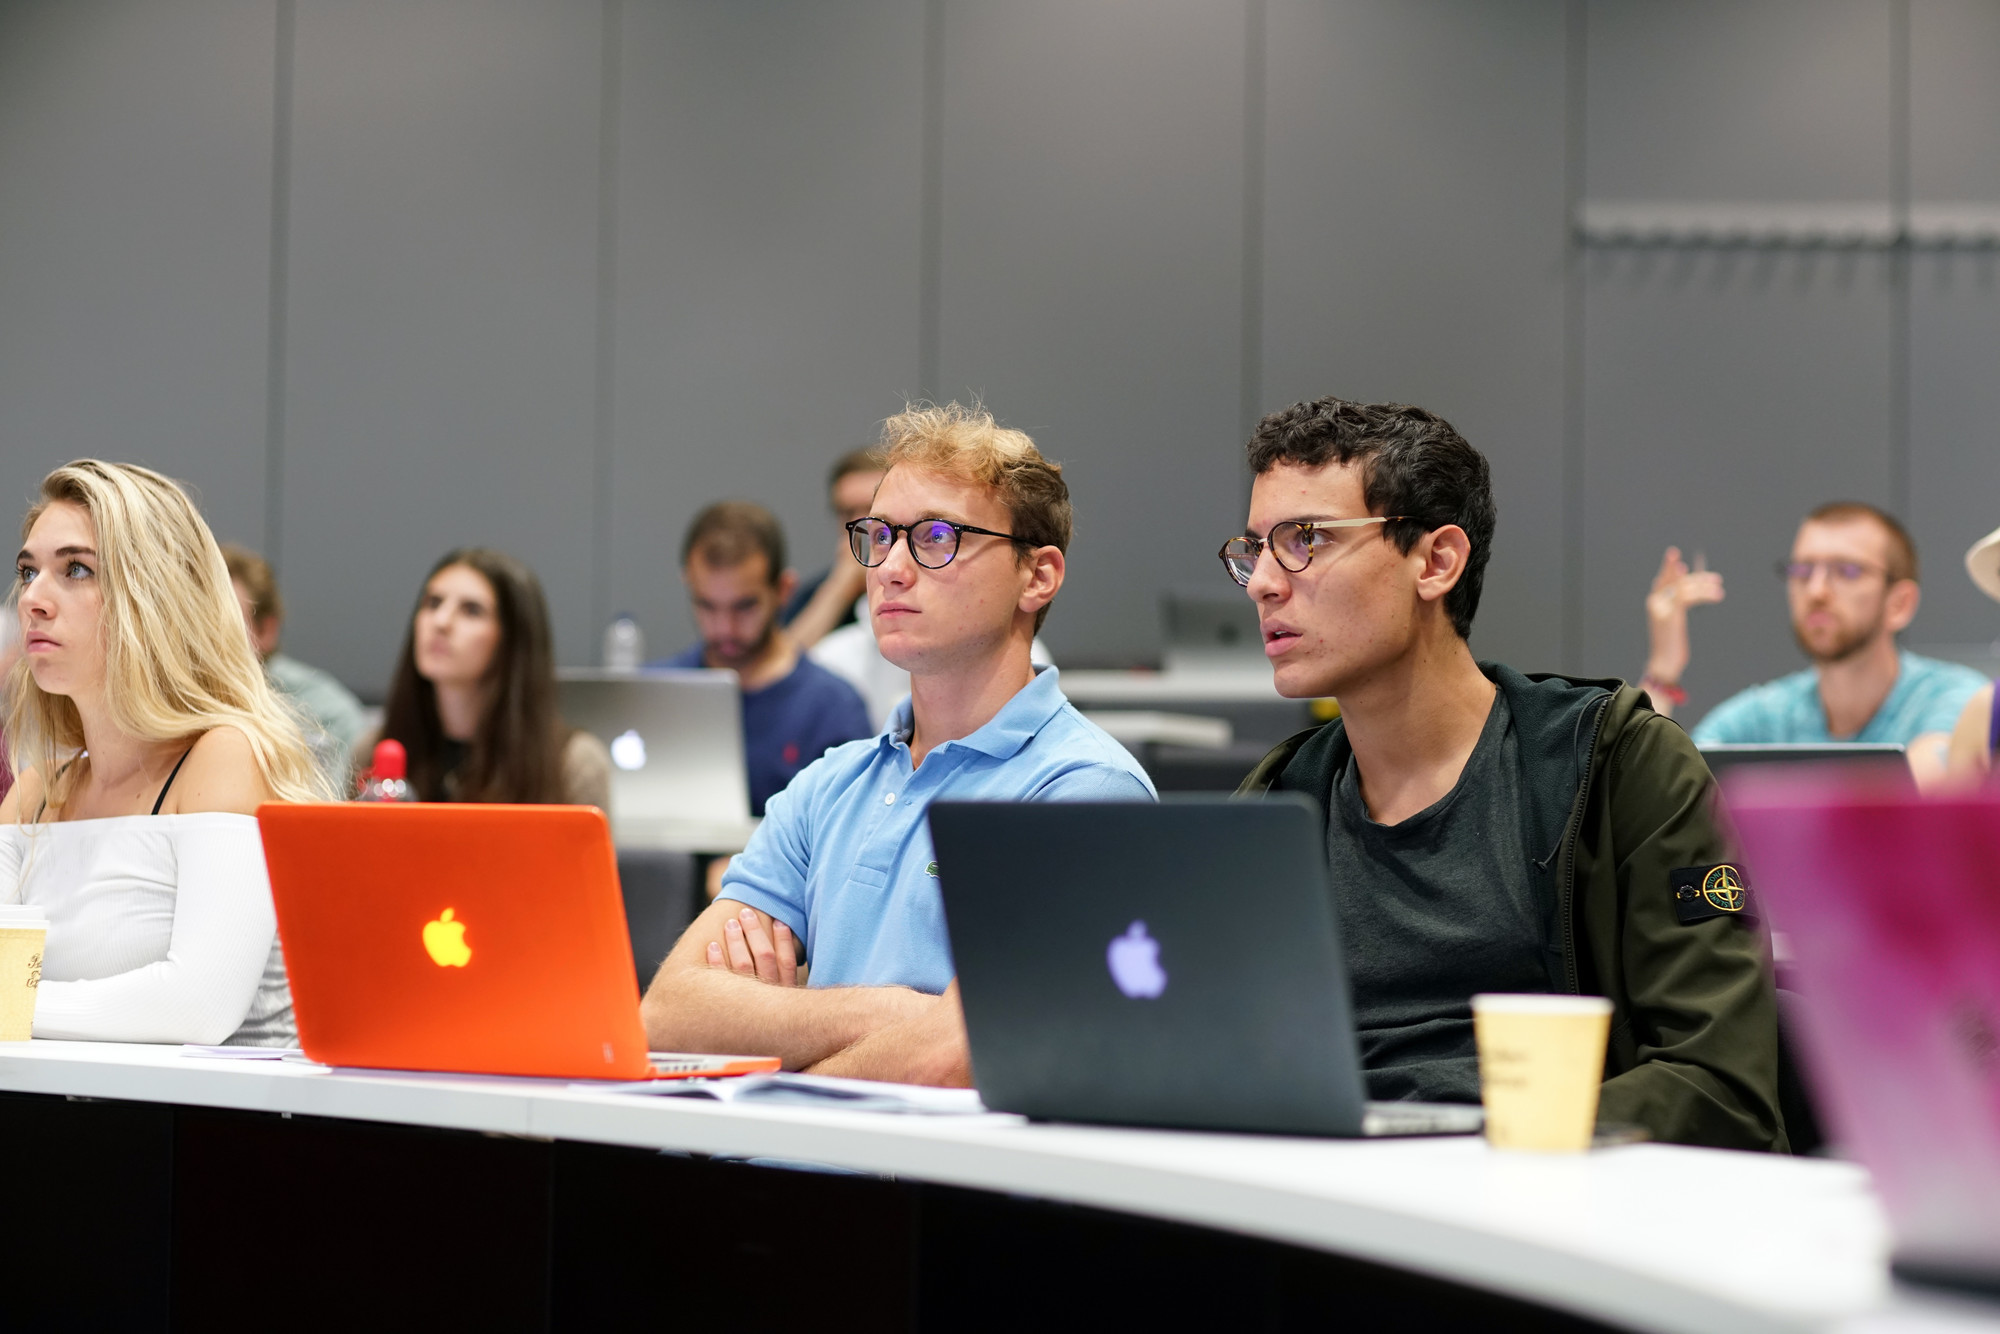
\includegraphics[width=\linewidth]{\imagefolder/abt_7295054328859831271Mjc0ODA1Ng.jpg}\\[3pt]
			\textbf{Section Title}\\			
			Sed et mincipidem am fugia ve nihi aut utatem invellupis dore voluptatiate veor olendi squatur?
	
			Ab illate sitate explibus reiundusam, voluptur sim idebit?
		\end{column}
		\begin{column}{0.3\linewidth} % Center column
			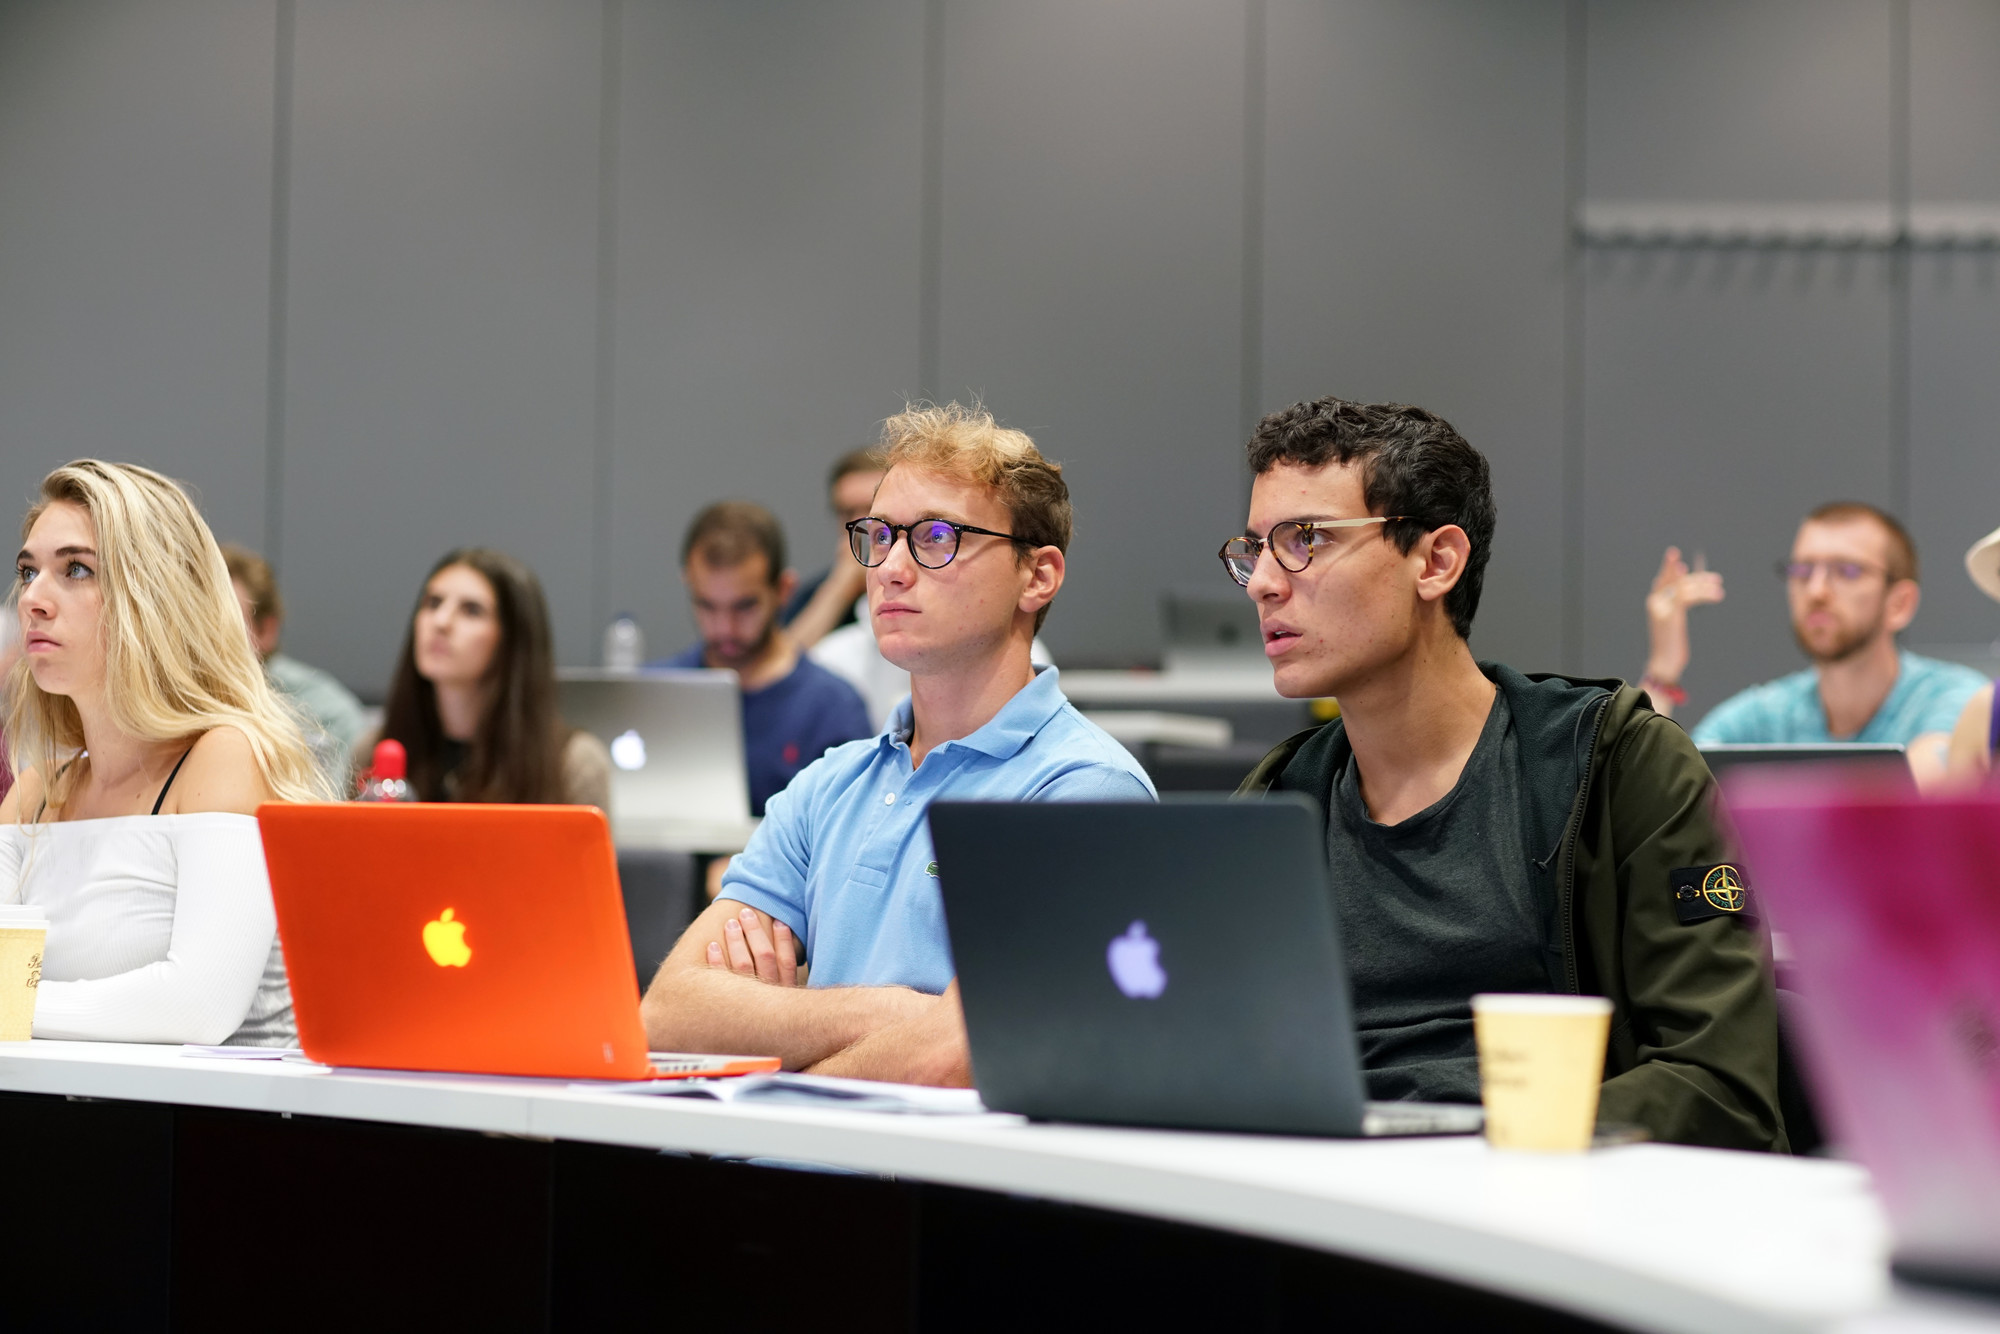
\includegraphics[width=\linewidth]{\imagefolder/abt_7295054328859831271Mjc0ODA1Ng.jpg}\\[3pt]
			\textbf{Section Title}\\			
			Sed et mincipidem am fugia ve nihi aut utatem invellupis dore voluptatiate veor olendi squatur?
	
			Ab illate sitate explibus reiundusam, voluptur sim idebit?
		\end{column}
		\begin{column}{0.3\linewidth} % Right column
			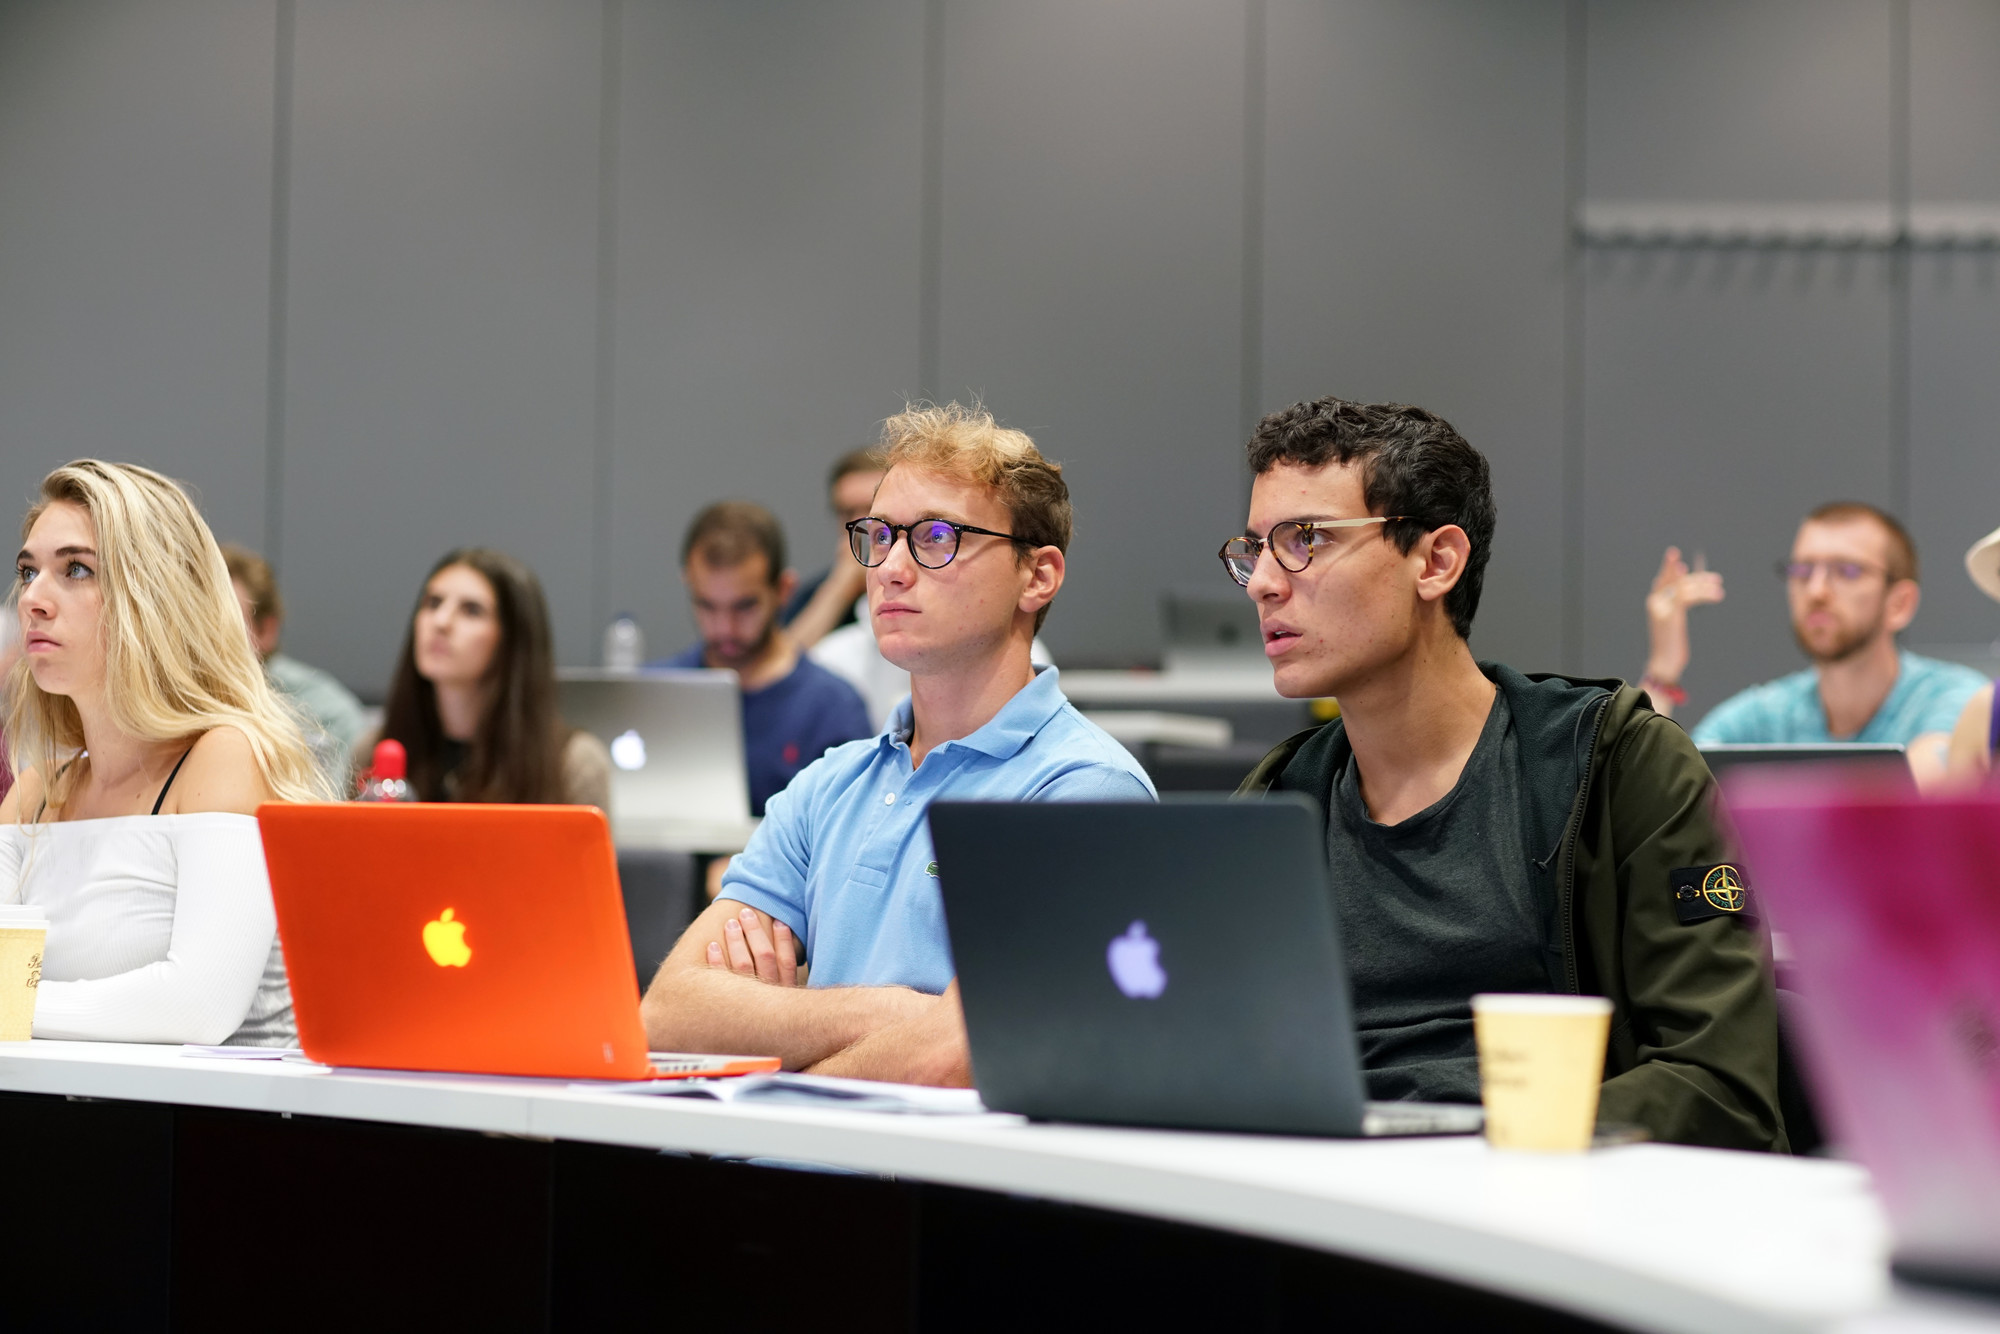
\includegraphics[width=\linewidth]{\imagefolder/abt_7295054328859831271Mjc0ODA1Ng.jpg}\\[3pt]
			\textbf{Section Title}\\			
			Sed et mincipidem am fugia ve nihi aut utatem invellupis dore voluptatiate veor olendi squatur?
	
			Ab illate sitate explibus reiundusam, voluptur sim idebit?
		\end{column}
	\end{columns}
\end{frame}

%------------------------------------------------

\begin{frame}
	\frametitle{Slide Title}
	\framesubtitle{Large Right Image Example}
	
	\begin{columns}[T] % [T] ensures correct vertical alignment
		\begin{column}{0.48\linewidth} % Left column
			\textbf{Section Title}
		
			Sed et mincipidem am fugia venihi aut utatem invellupis dolore voluptatiate veor mo dolendi squatur?

			Ab illate sitate explibus reiundusam, voluptur sim idebit, omnis dero quas adio quatur?

			Pa cumquat ute nos exero magnime officatem. Luptia voluptatur aut acia comnist qui beatusam, omniatecae iur alit, cus debis
		\end{column}
		\begin{column}{0.48\linewidth} % Right column
			\vspace{-3.5\baselineskip} % Pull image up
			
			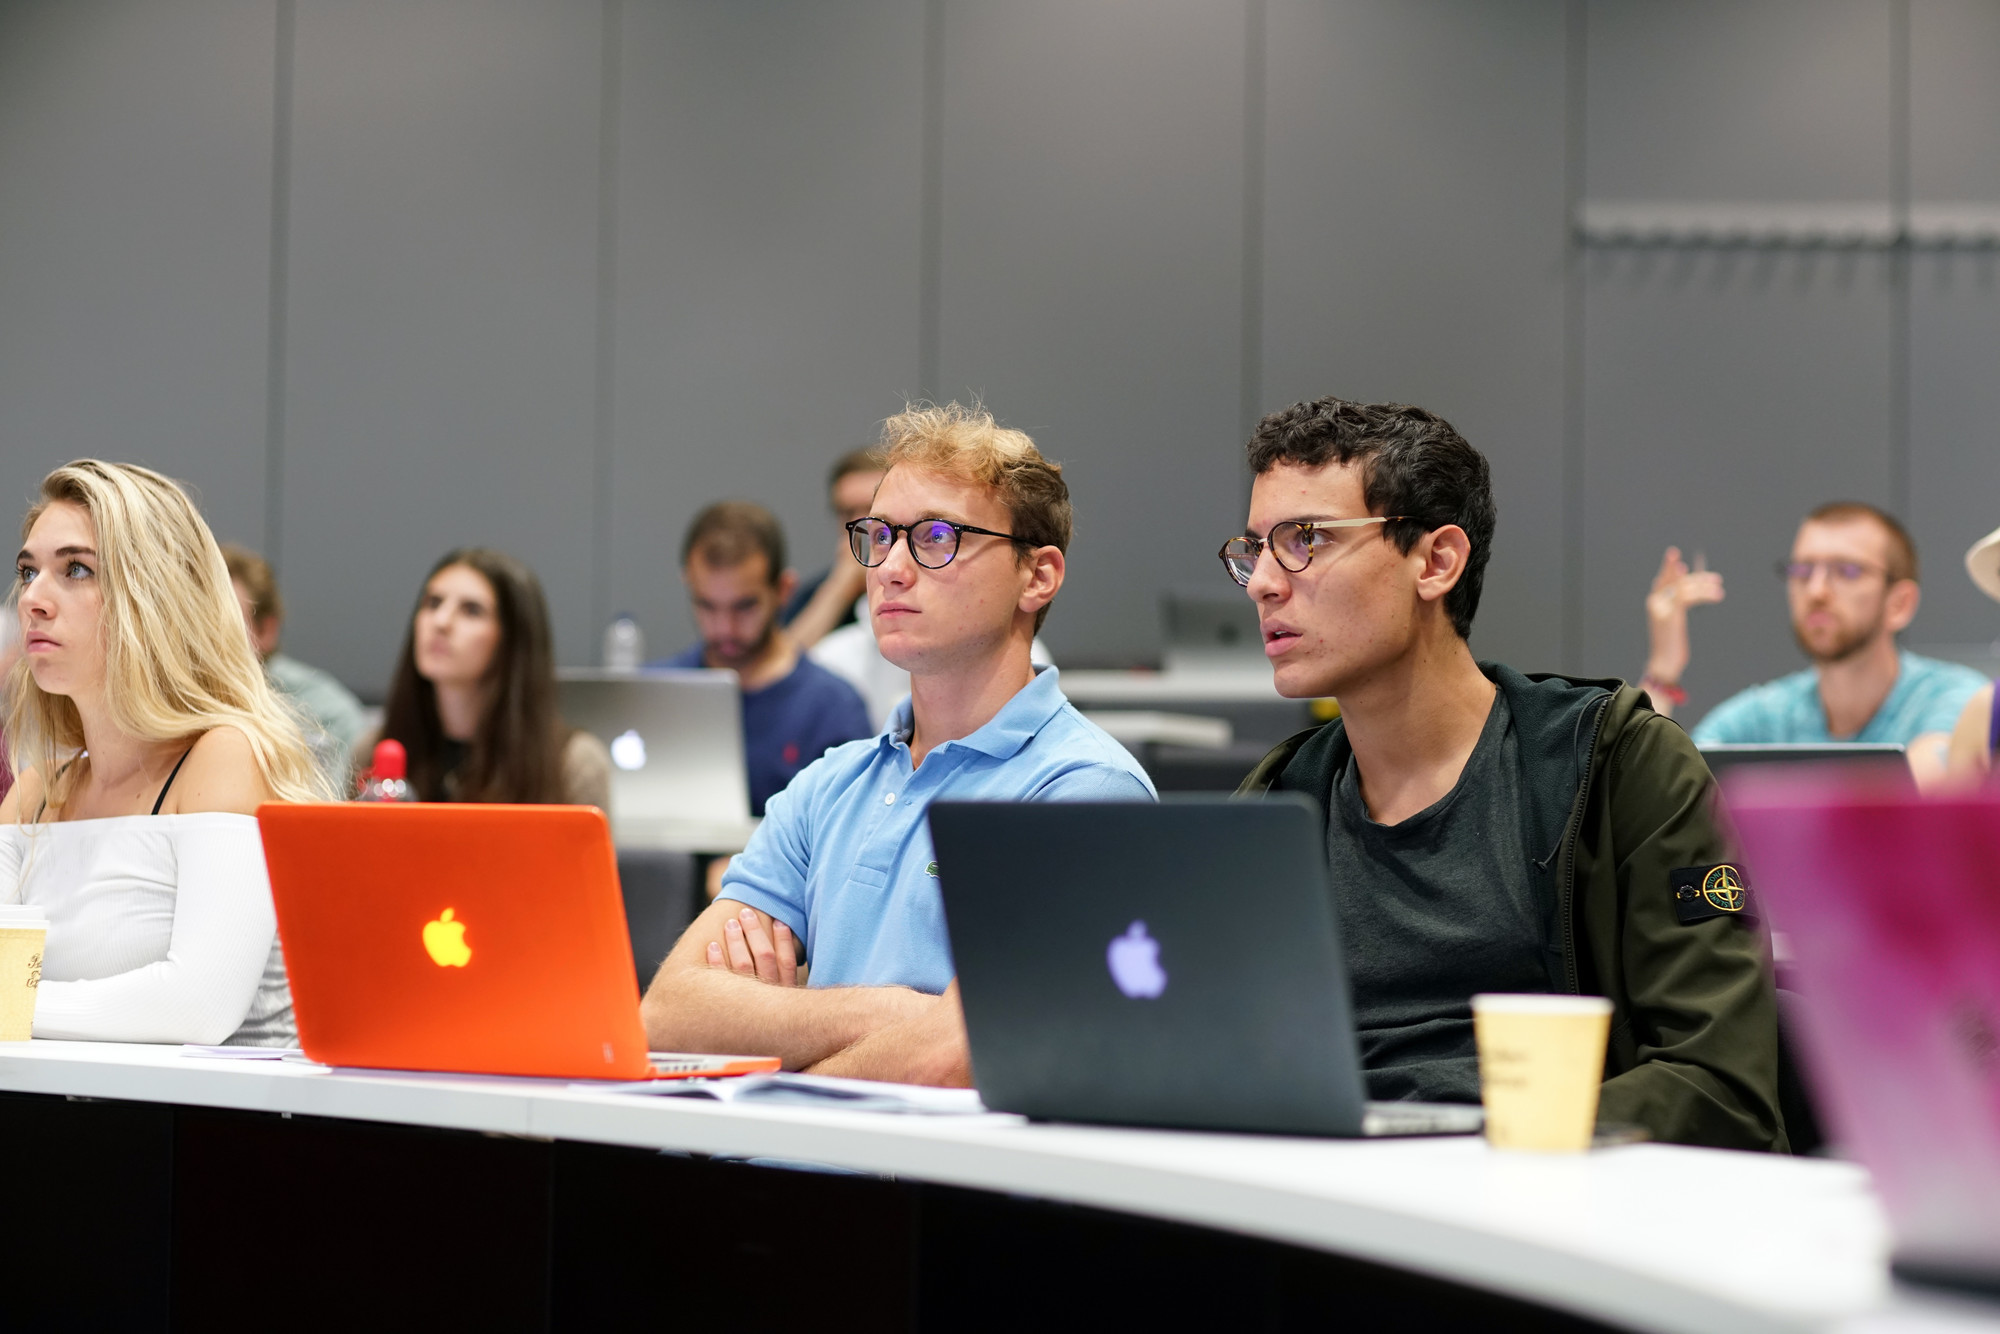
\includegraphics[trim=3cm 0cm 3cm 1cm, clip, width=\linewidth]{\imagefolder/abt_7295054328859831271Mjc0ODA1Ng.jpg} % Trimming is used to crop your image and the order of dimensions is: left, bottom, right, top. It's recommended to crop outside of LaTeX though, to ensure the aspect ratio remains the same.
			{\tiny\textcolor{ICLBlue}{(Above) Photography Credit or Caption}}
		\end{column}
	\end{columns}
\end{frame}

%------------------------------------------------

\begin{frame}
	\begin{columns}[T] % [T] ensures correct vertical alignment
		\begin{column}{0.48\linewidth} % Left column			
			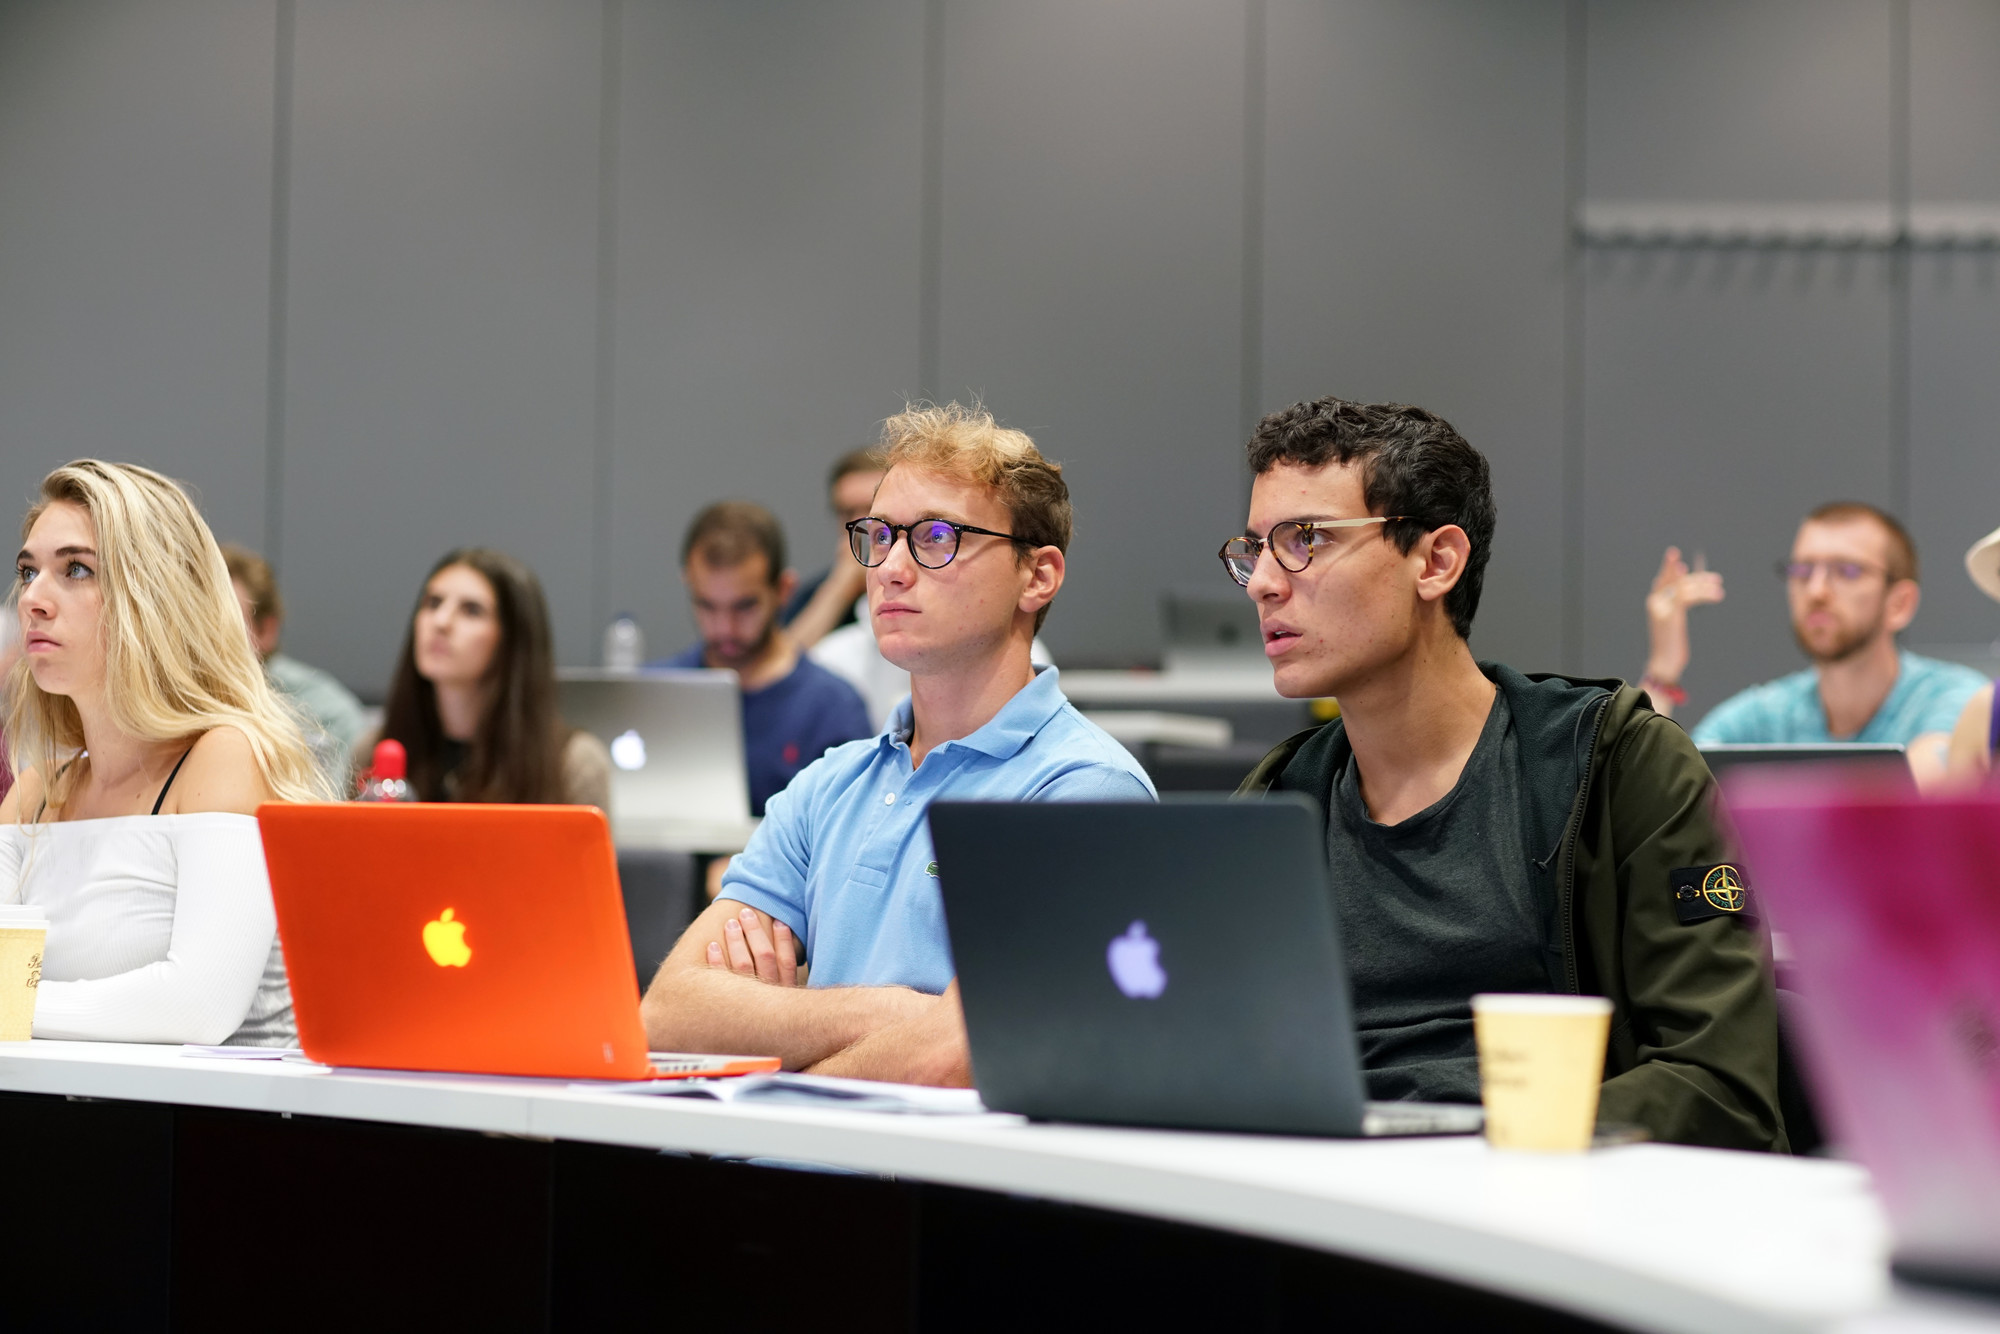
\includegraphics[trim=3cm 0cm 3cm 1cm, clip, width=\linewidth]{\imagefolder/abt_7295054328859831271Mjc0ODA1Ng.jpg} % Trimming is used to crop your image and the order of dimensions is: left, bottom, right, top. It's recommended to crop outside of LaTeX though, to ensure the aspect ratio remains the same.
			{\tiny\textcolor{ICLBlue}{(Above) Photography Credit or Caption}}
		\end{column}
		\begin{column}{0.48\linewidth} % Right column
			\textbf{Section Title}\\
			Sed et mincipidem am fugia venihi aut utatem invellupis dolore voluptatiate veor mo dolendi squatur?

			Ab illate sitate explibus reiundusam, voluptur sim idebit, omnis dero quas adio quatur?

			Pa cumquat ute nos exero magnime officatem. Luptia voluptatur aut acia comnist qui beatusam, omniatecae iur alit, cus debis
		\end{column}
	\end{columns}
\end{frame}

%------------------------------------------------

\begin{frame}
	\begin{columns}[T] % [T] ensures correct vertical alignment
		\begin{column}{0.48\linewidth} % Left column
			\textbf{Section Title}\\
			Sed et mincipidem am fugia venihi aut utatem invellupis dolore voluptatiate veor mo dolendi squatur?

			Ab illate sitate explibus reiundusam, voluptur sim idebit, omnis dero quas adio quatur?

			Pa cumquat ute nos exero magnime officatem. Luptia voluptatur aut acia comnist qui beatusam, omniatecae iur alit, cus debis
		\end{column}
		\begin{column}{0.48\linewidth} % Right column			
			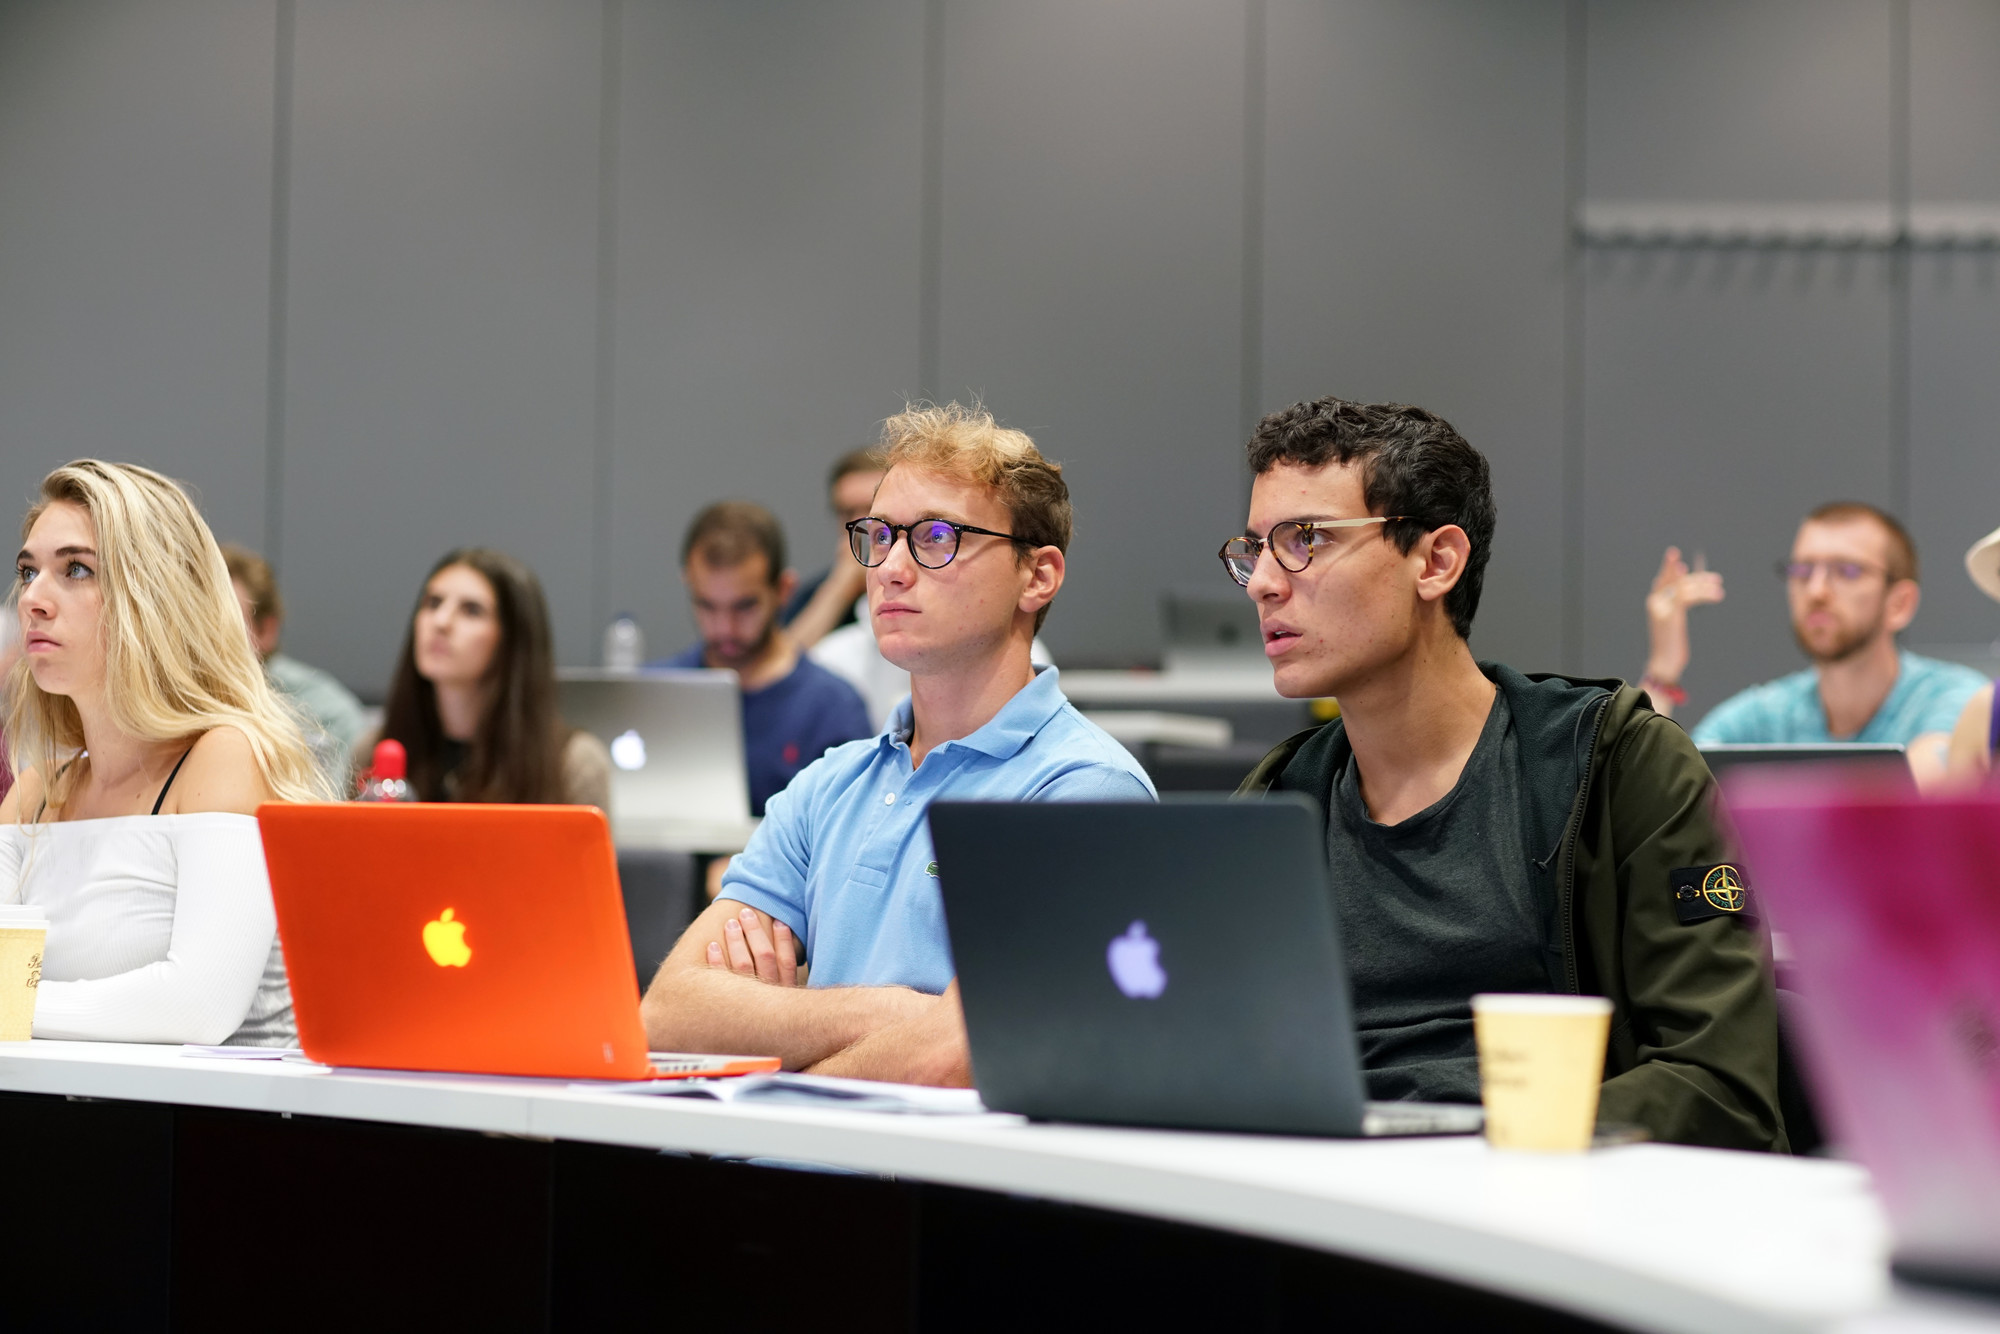
\includegraphics[trim=3cm 0cm 3cm 1cm, clip, width=\linewidth]{\imagefolder/abt_7295054328859831271Mjc0ODA1Ng.jpg} % Trimming is used to crop your image and the order of dimensions is: left, bottom, right, top. It's recommended to crop outside of LaTeX though, to ensure the aspect ratio remains the same.
			{\tiny\textcolor{ICLBlue}{(Above) Photography Credit or Caption}}
		\end{column}
	\end{columns}
\end{frame}

%------------------------------------------------

\begin{frame}
	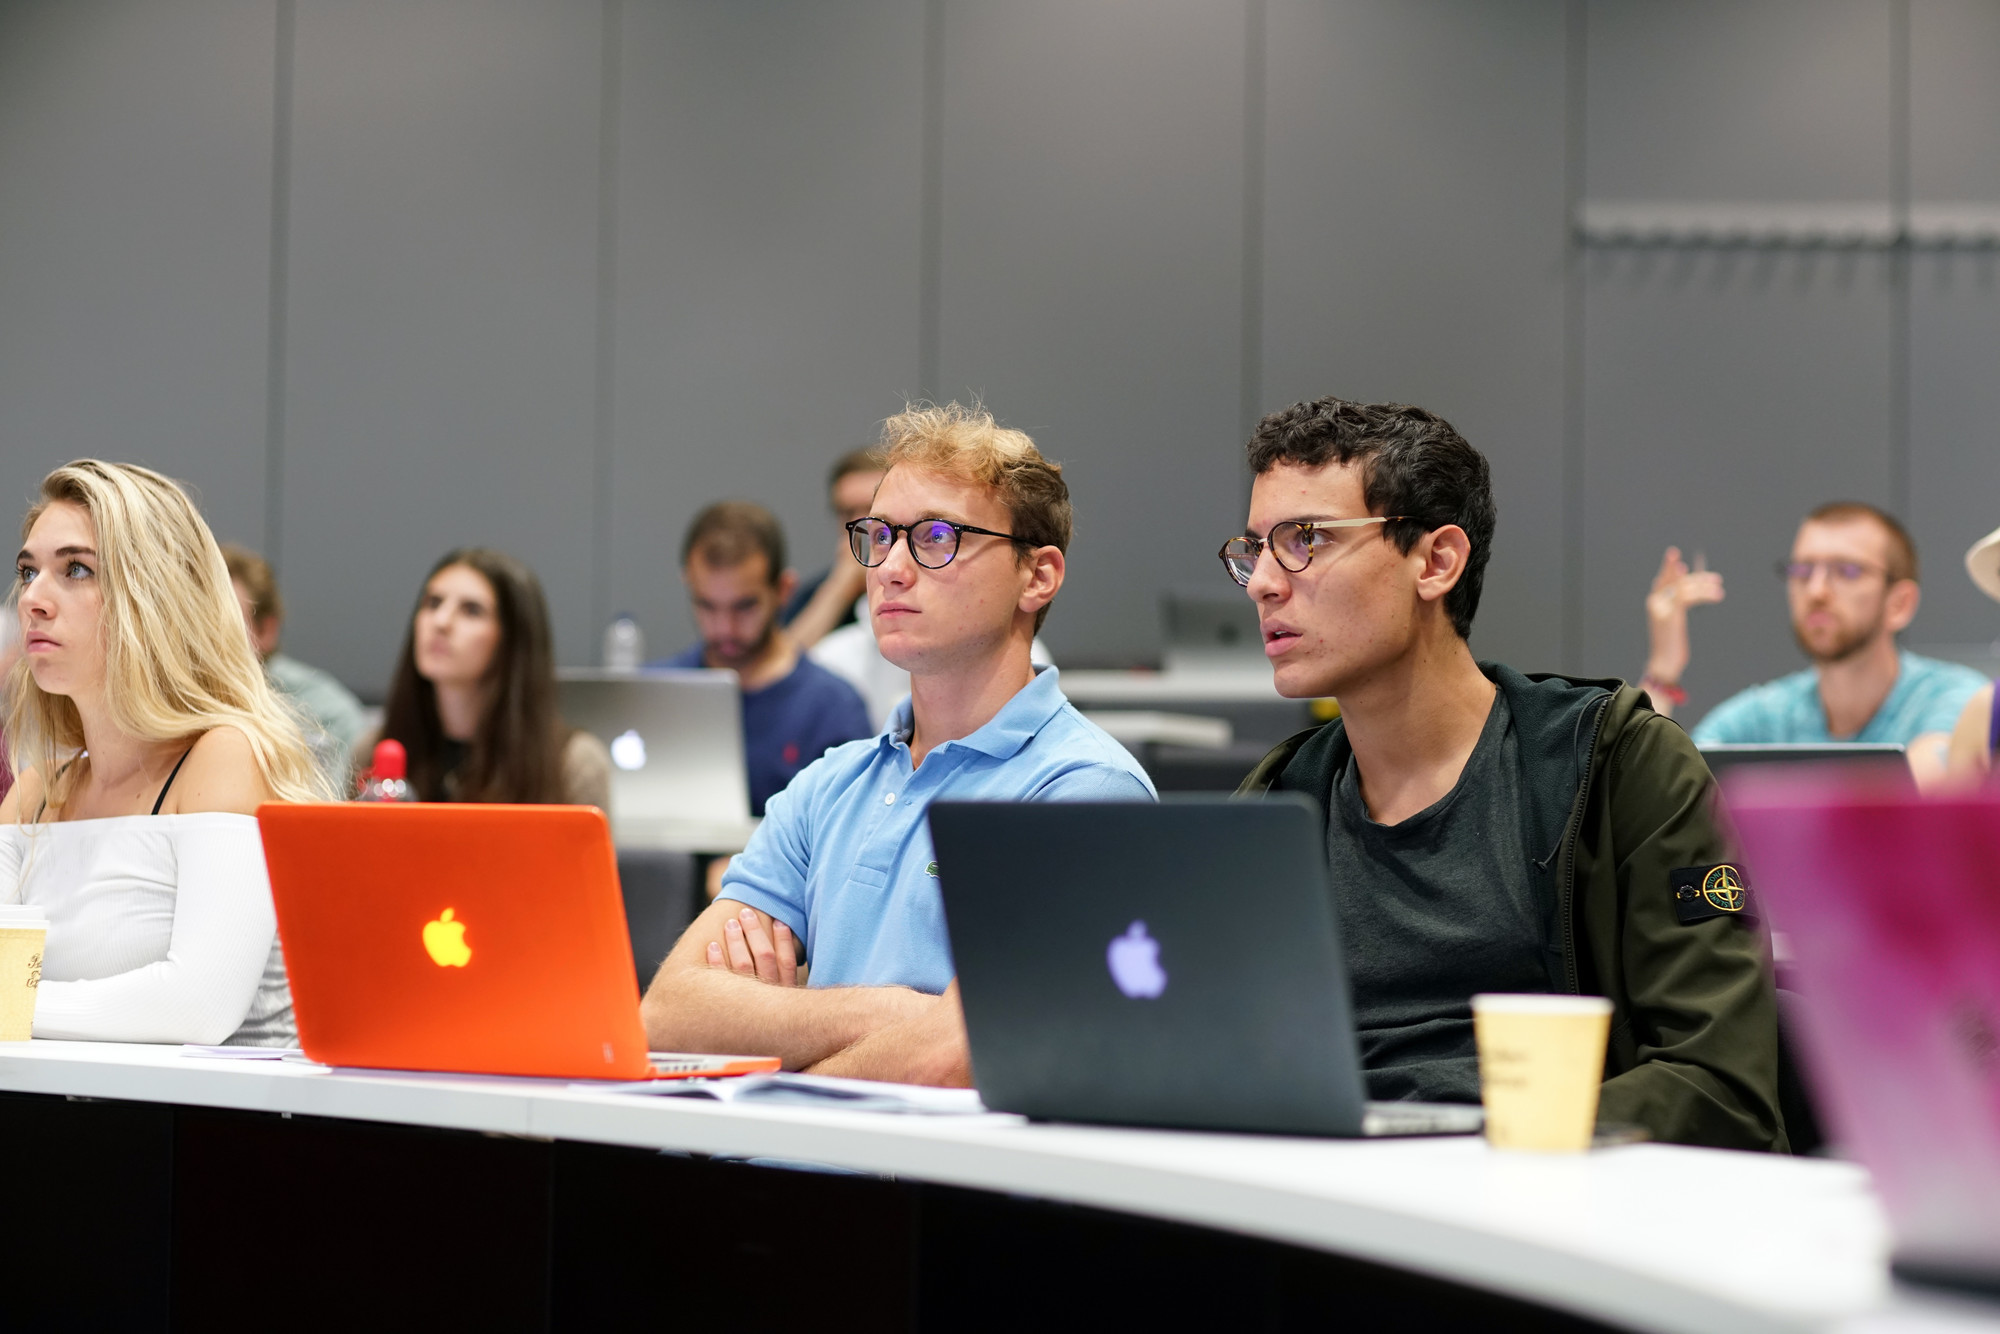
\includegraphics[trim=0cm 1.5cm 0cm 1.5cm, clip, width=\linewidth, height=\textheight]{\imagefolder/abt_7295054328859831271Mjc0ODA1Ng.jpg} % Trimming is used to crop your image and the order of dimensions is: left, bottom, right, top. It's recommended to crop outside of LaTeX though, to ensure the aspect ratio remains the same.
\end{frame}

%------------------------------------------------

\begingroup
	\setbeamertemplate{background}{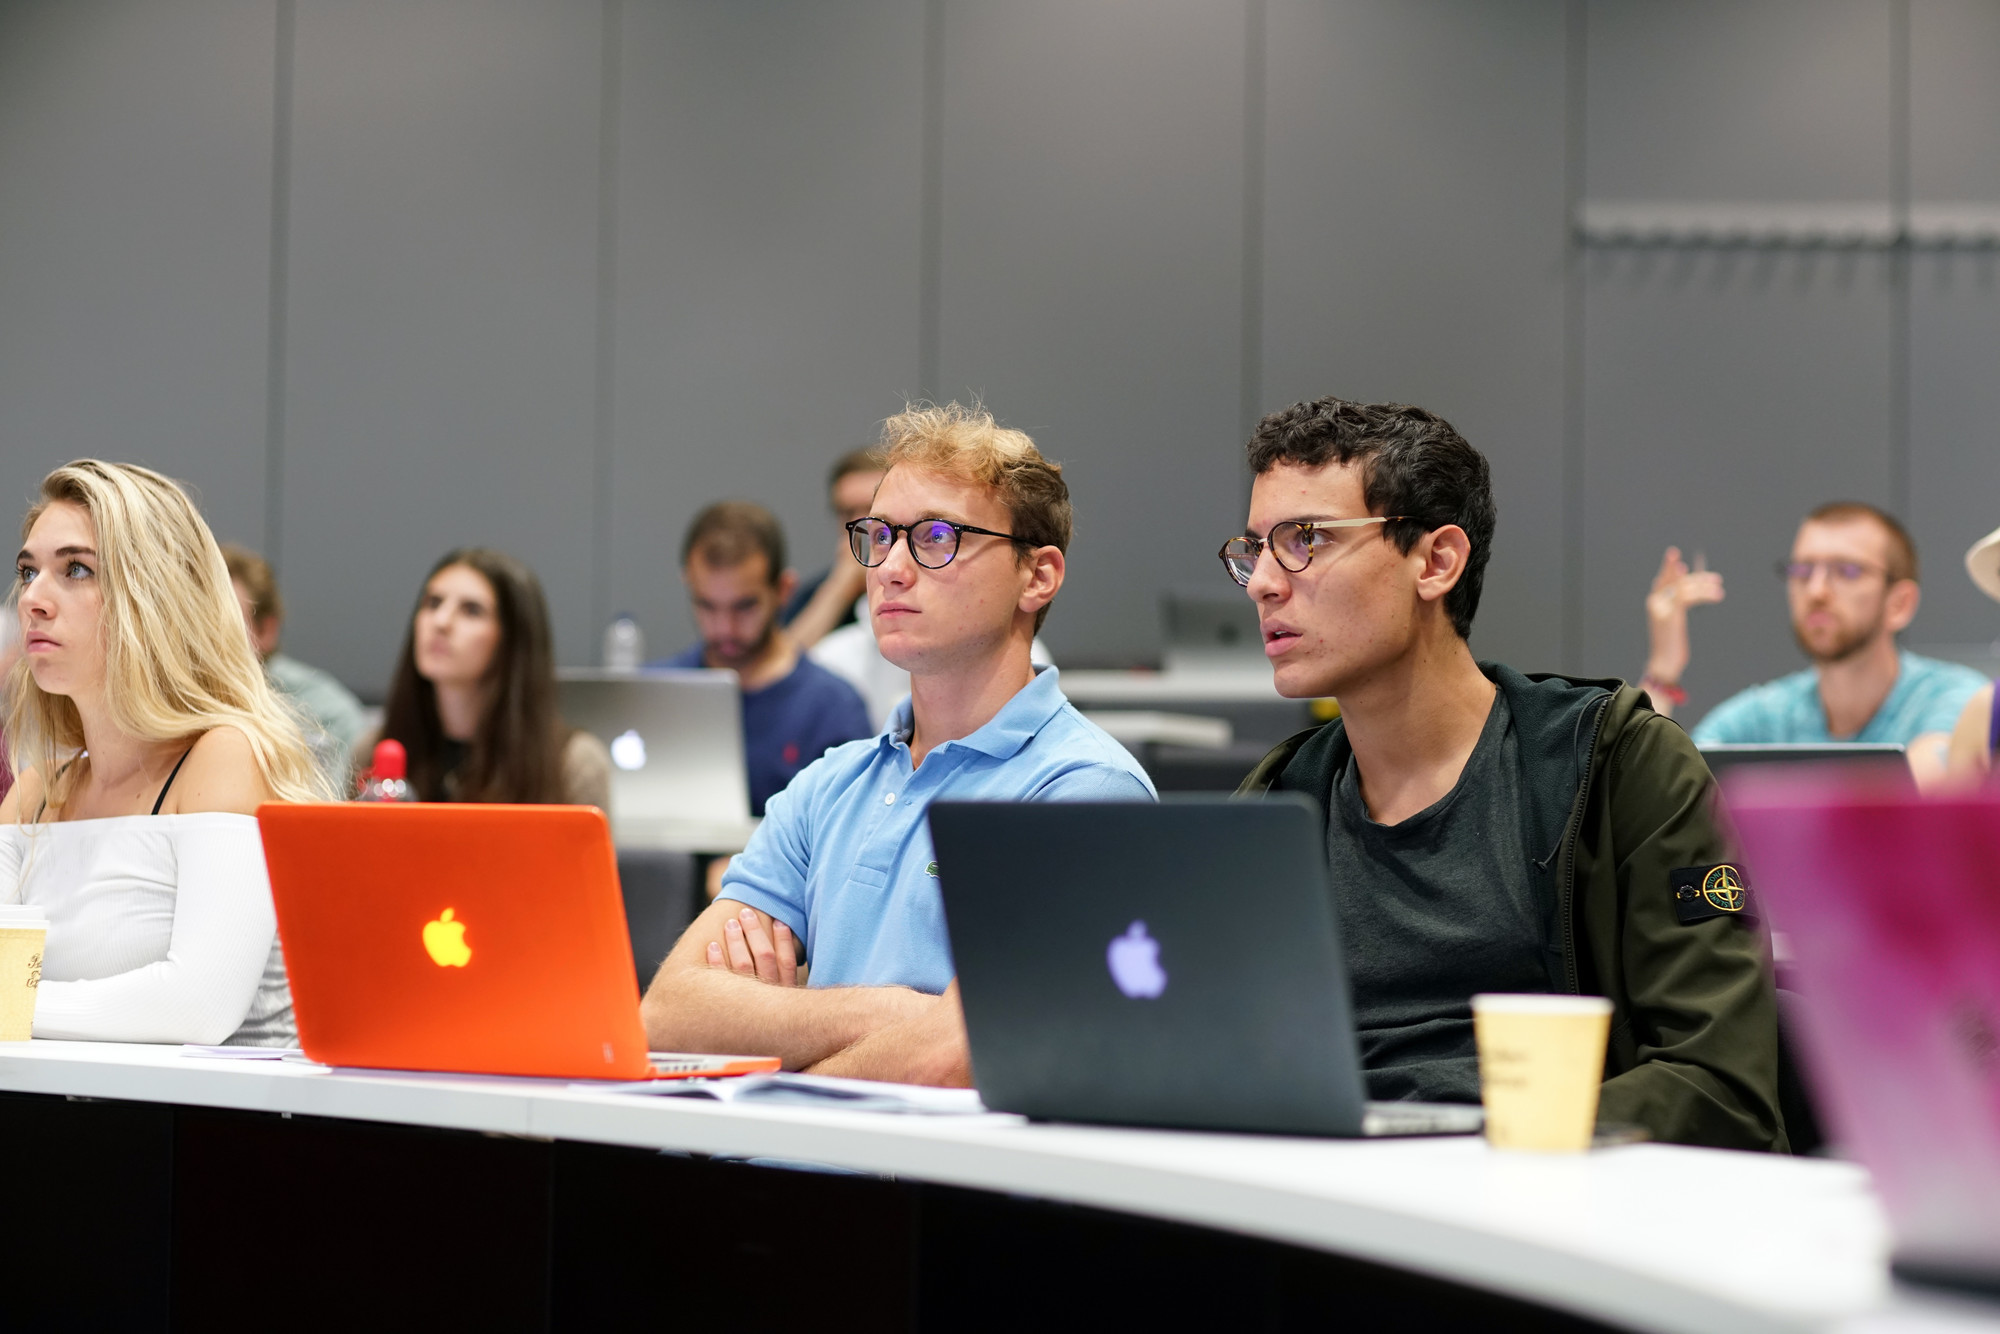
\includegraphics[width=\paperwidth]{\imagefolder/abt_7295054328859831271Mjc0ODA1Ng.jpg}} % Slide background image
	
	\begin{frame}[plain] % 'plain' suppresses the footer
	\end{frame}
\endgroup

%------------------------------------------------

\begingroup
	\setbeamertemplate{background}{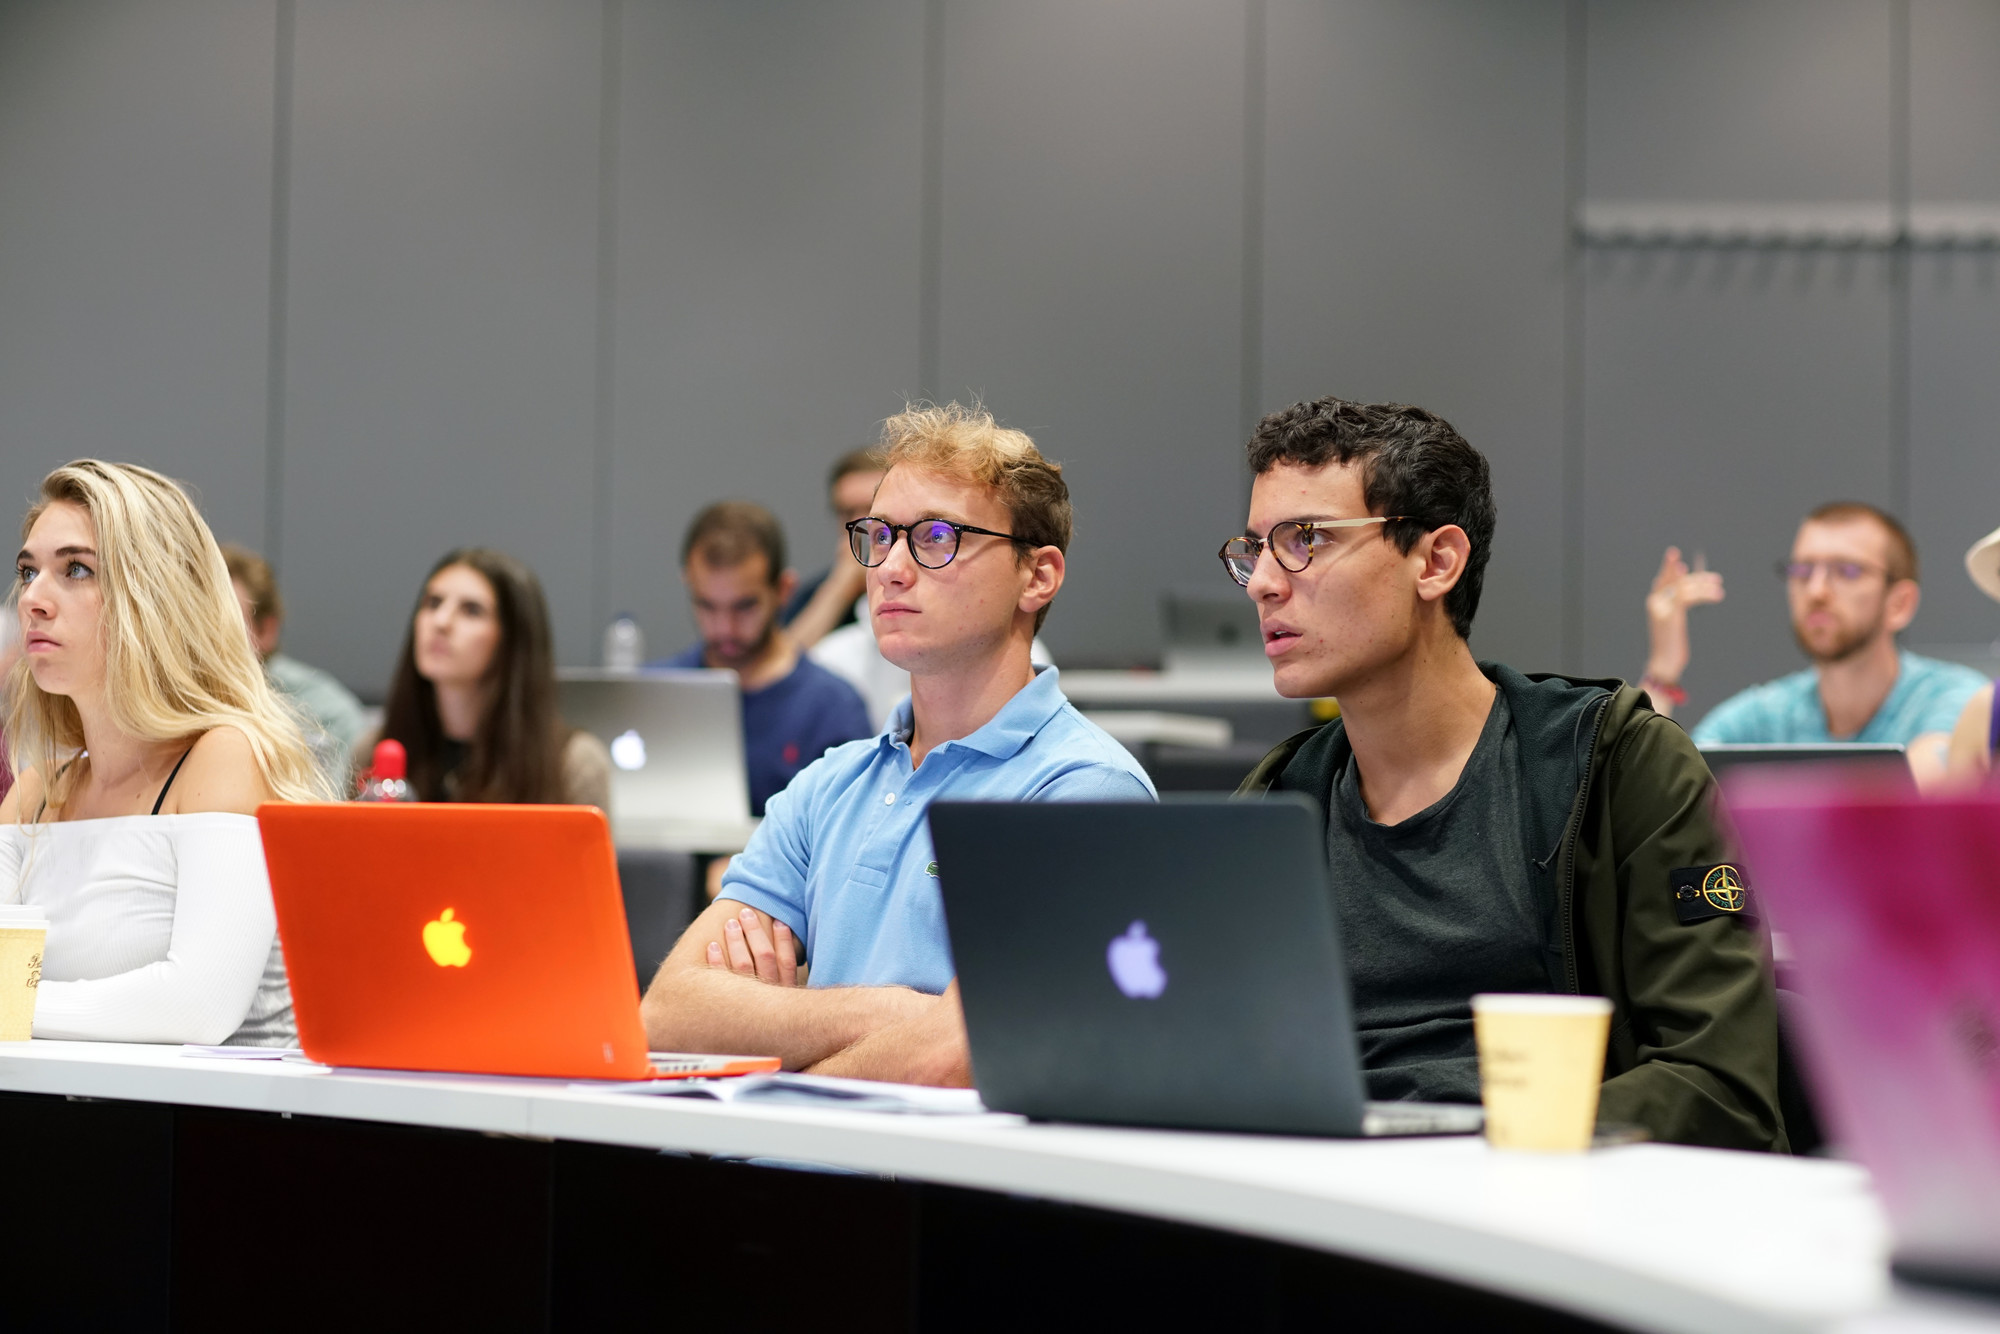
\includegraphics[width=\paperwidth]{\imagefolder/abt_7295054328859831271Mjc0ODA1Ng.jpg}} % Slide background image
	\setbeamercolor{normal text}{fg=white}\usebeamercolor[fg]{normal text} % Slide text color
	\setbeamercolor{page number in head/foot}{fg=white} % Footer text color
	
	\begin{frame}
		Text can be included on slides with image backgrounds too.
	\end{frame}
\endgroup

%------------------------------------------------

\begin{frame}
	\frametitle{Slide Title}
	\framesubtitle{Tiled Images Example}
	
	\small % Reduce font size in this slide
	
	\begin{columns}[T] % [T] ensures correct vertical alignment
		\begin{column}{0.3\linewidth} % Left column
			\textbf{Section Title}\\
			Sed et mincipidem am fugia venihi aut utatem invellupis dolore voluptatiate veor mo dolendi squatur?

			Ab illate sitate explibus reiundusam, voluptur sim idebit, omnis dero quas adio quatur?
		\end{column}
		\begin{column}{0.68\linewidth} % Right column
			\vspace{-3.5\baselineskip} % Pull images up
			
			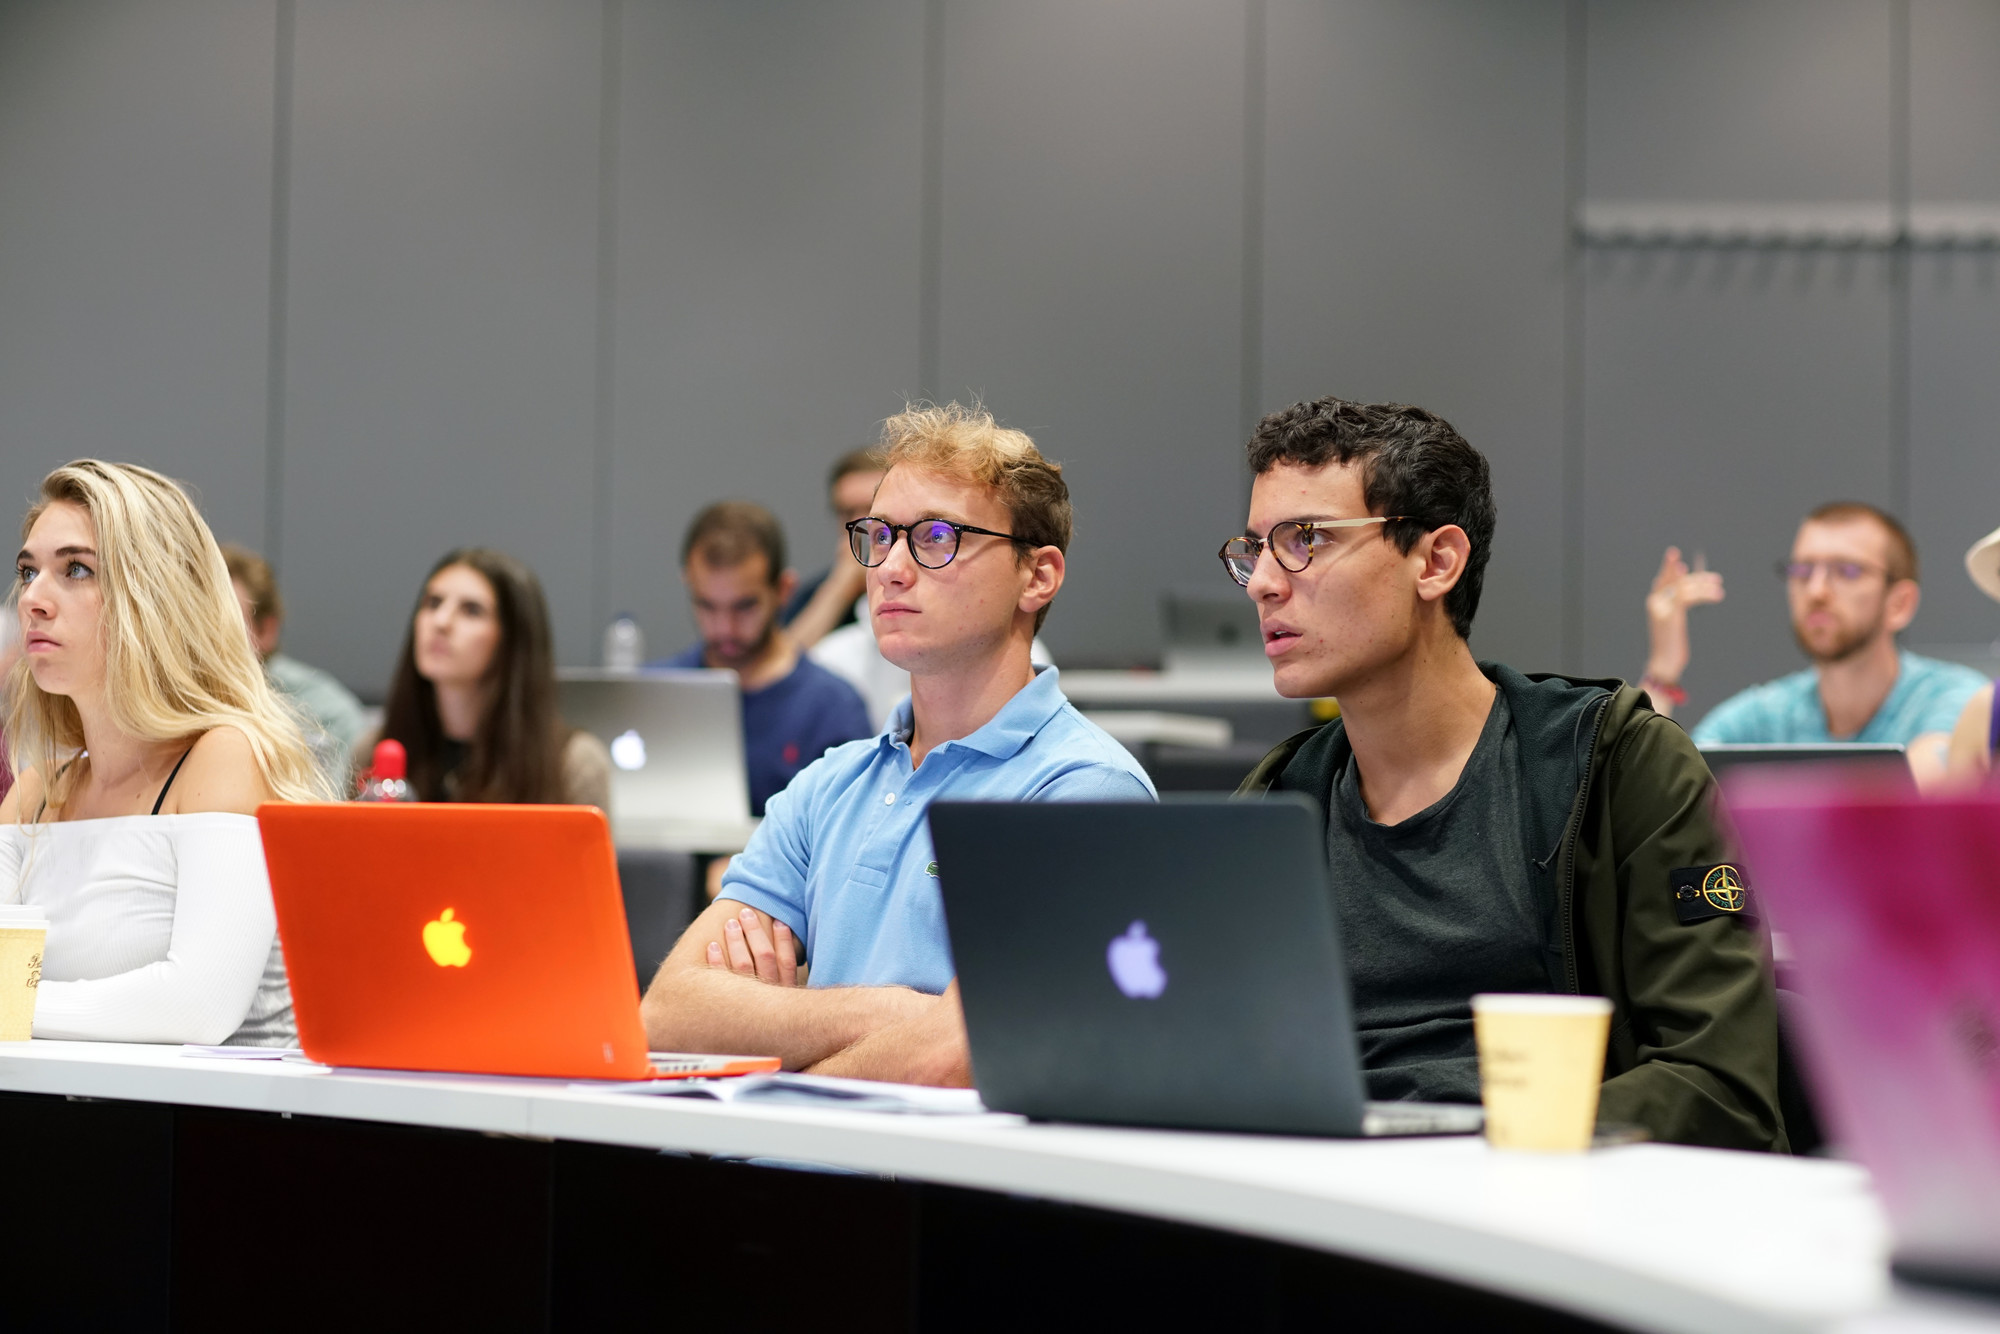
\includegraphics[width=0.32\linewidth]{\imagefolder/abt_7295054328859831271Mjc0ODA1Ng.jpg}\hfill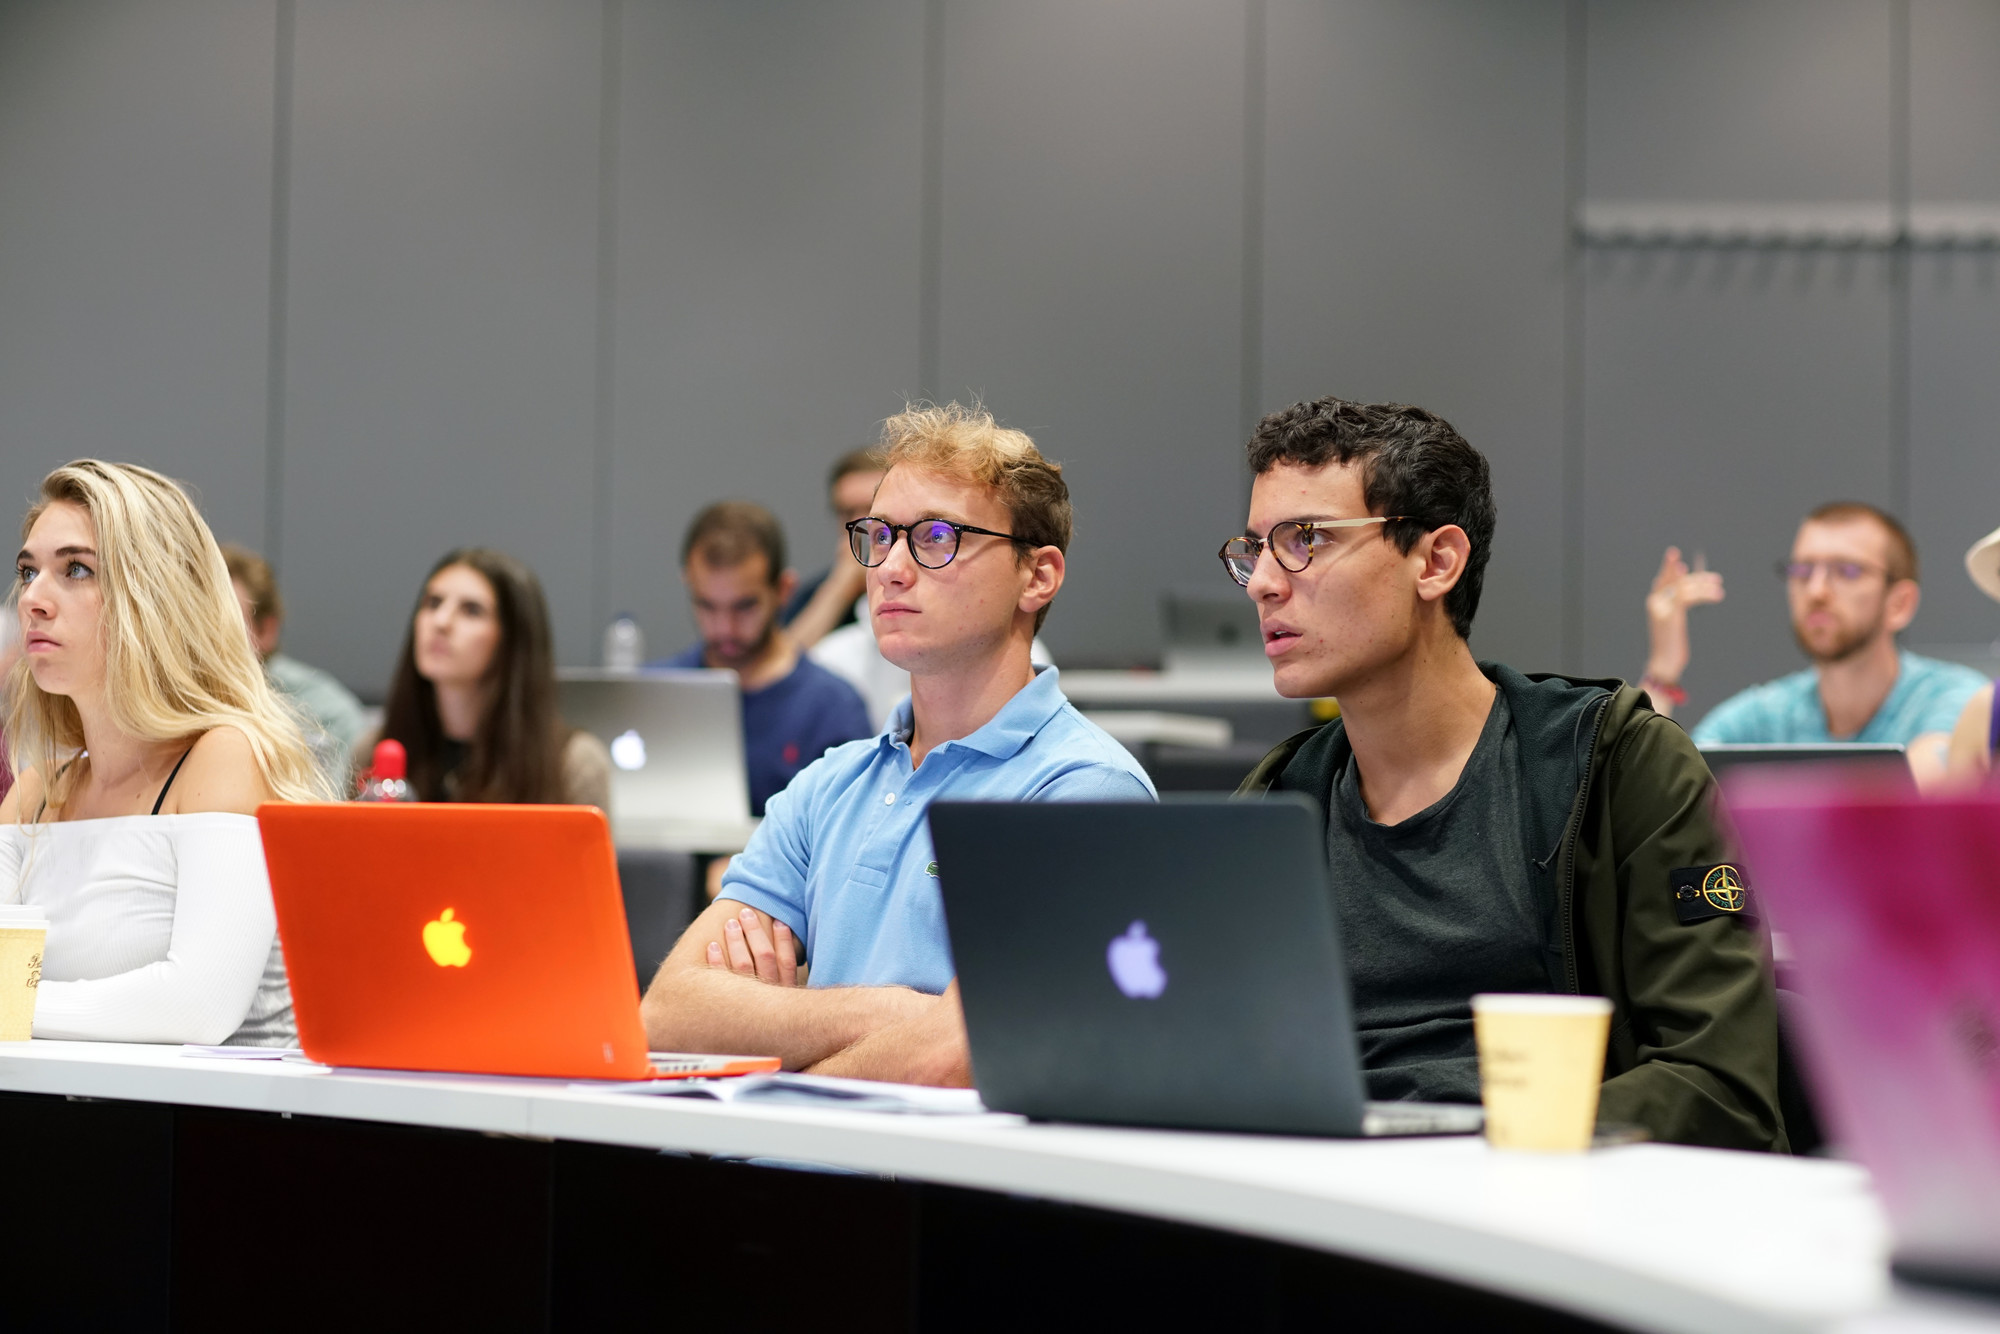
\includegraphics[width=0.32\linewidth]{\imagefolder/abt_7295054328859831271Mjc0ODA1Ng.jpg}\hfill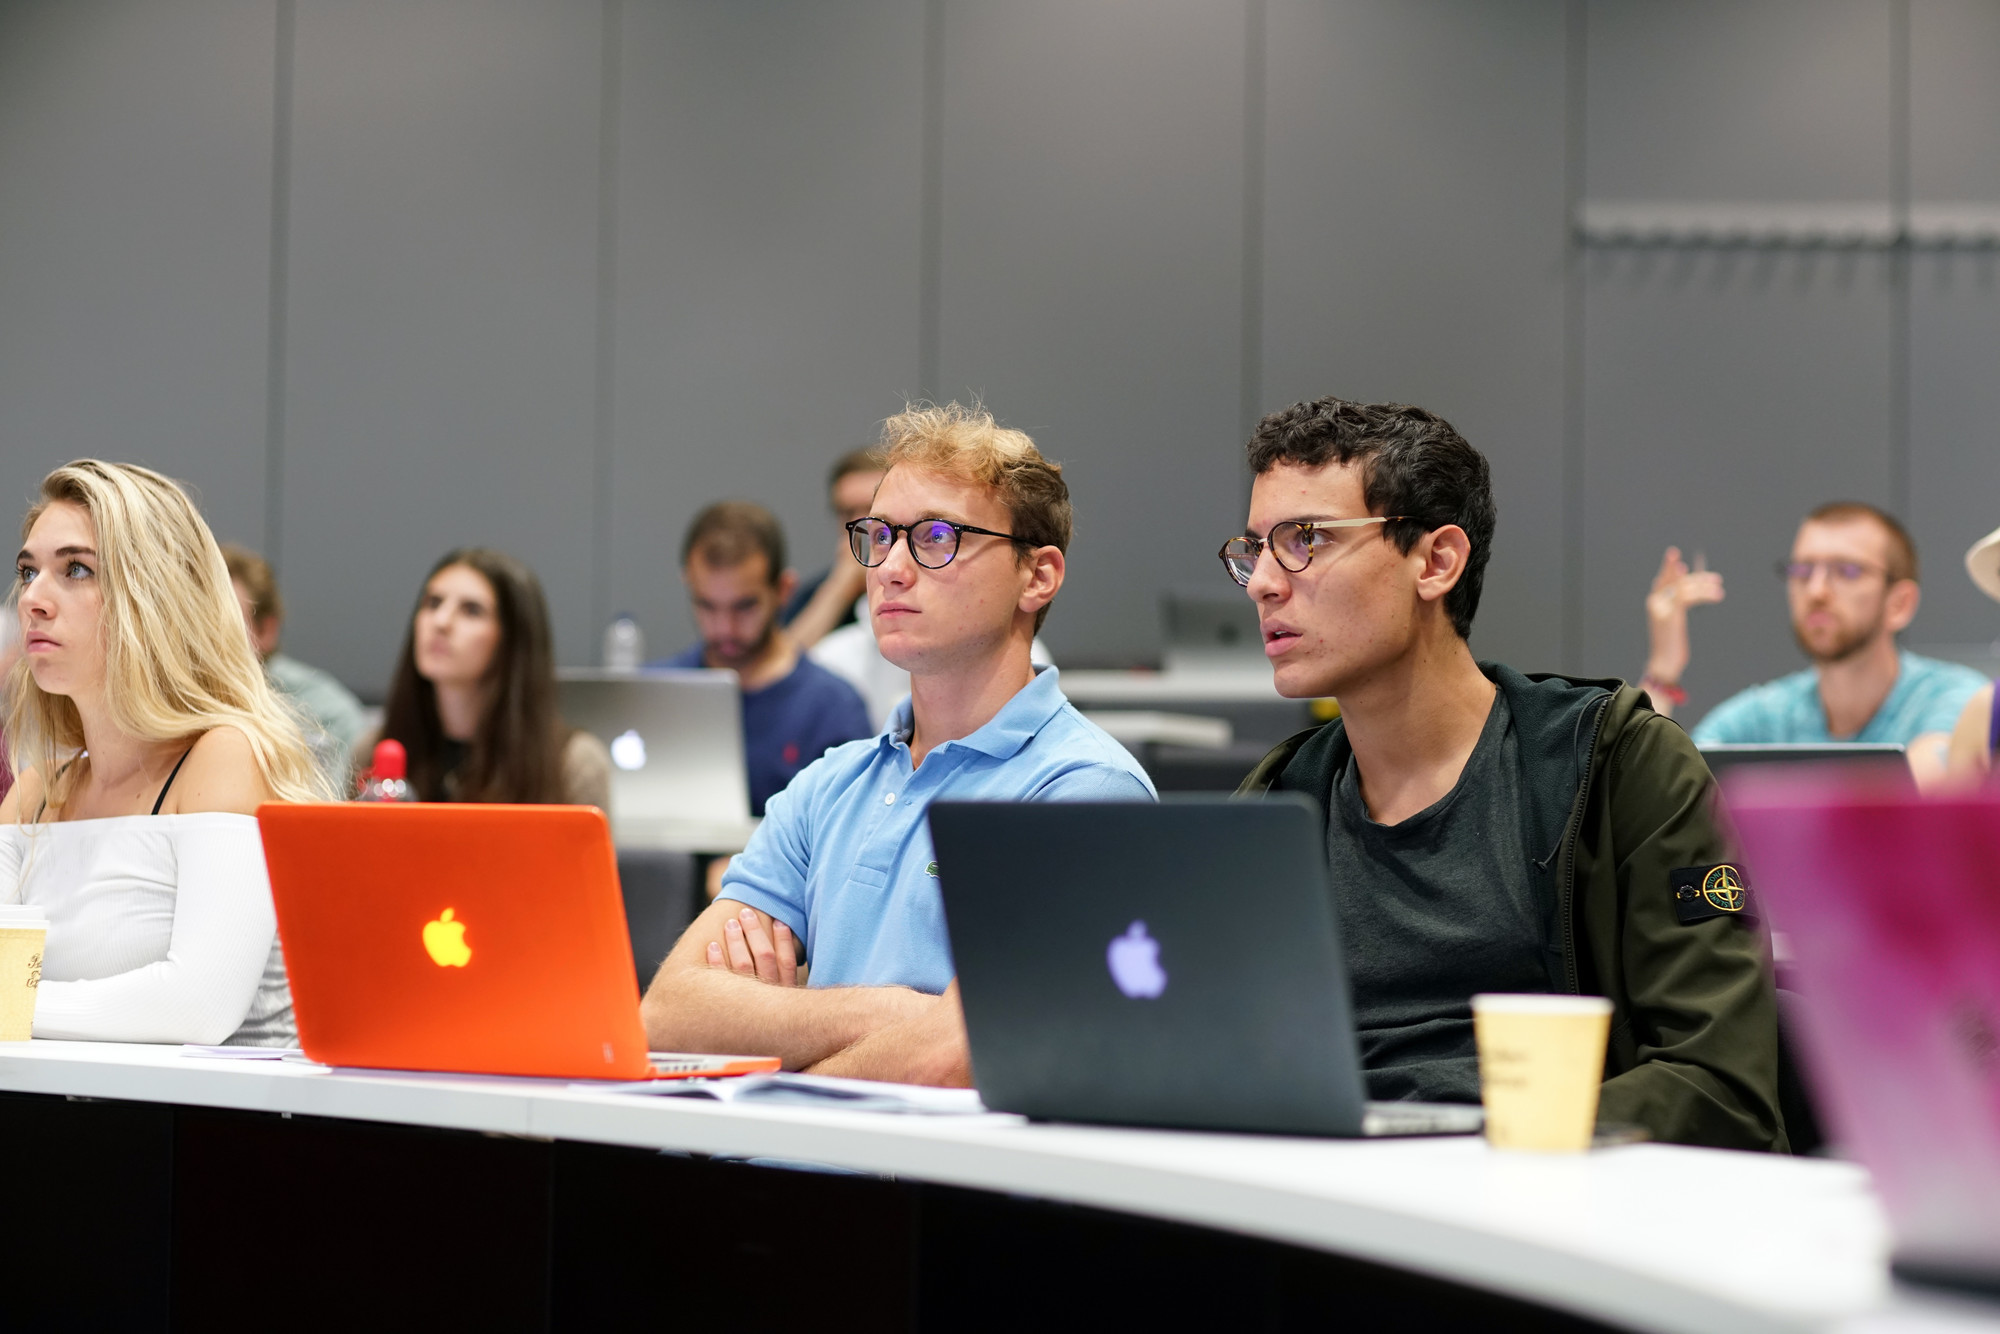
\includegraphics[width=0.32\linewidth]{\imagefolder/abt_7295054328859831271Mjc0ODA1Ng.jpg}\\[6pt]
			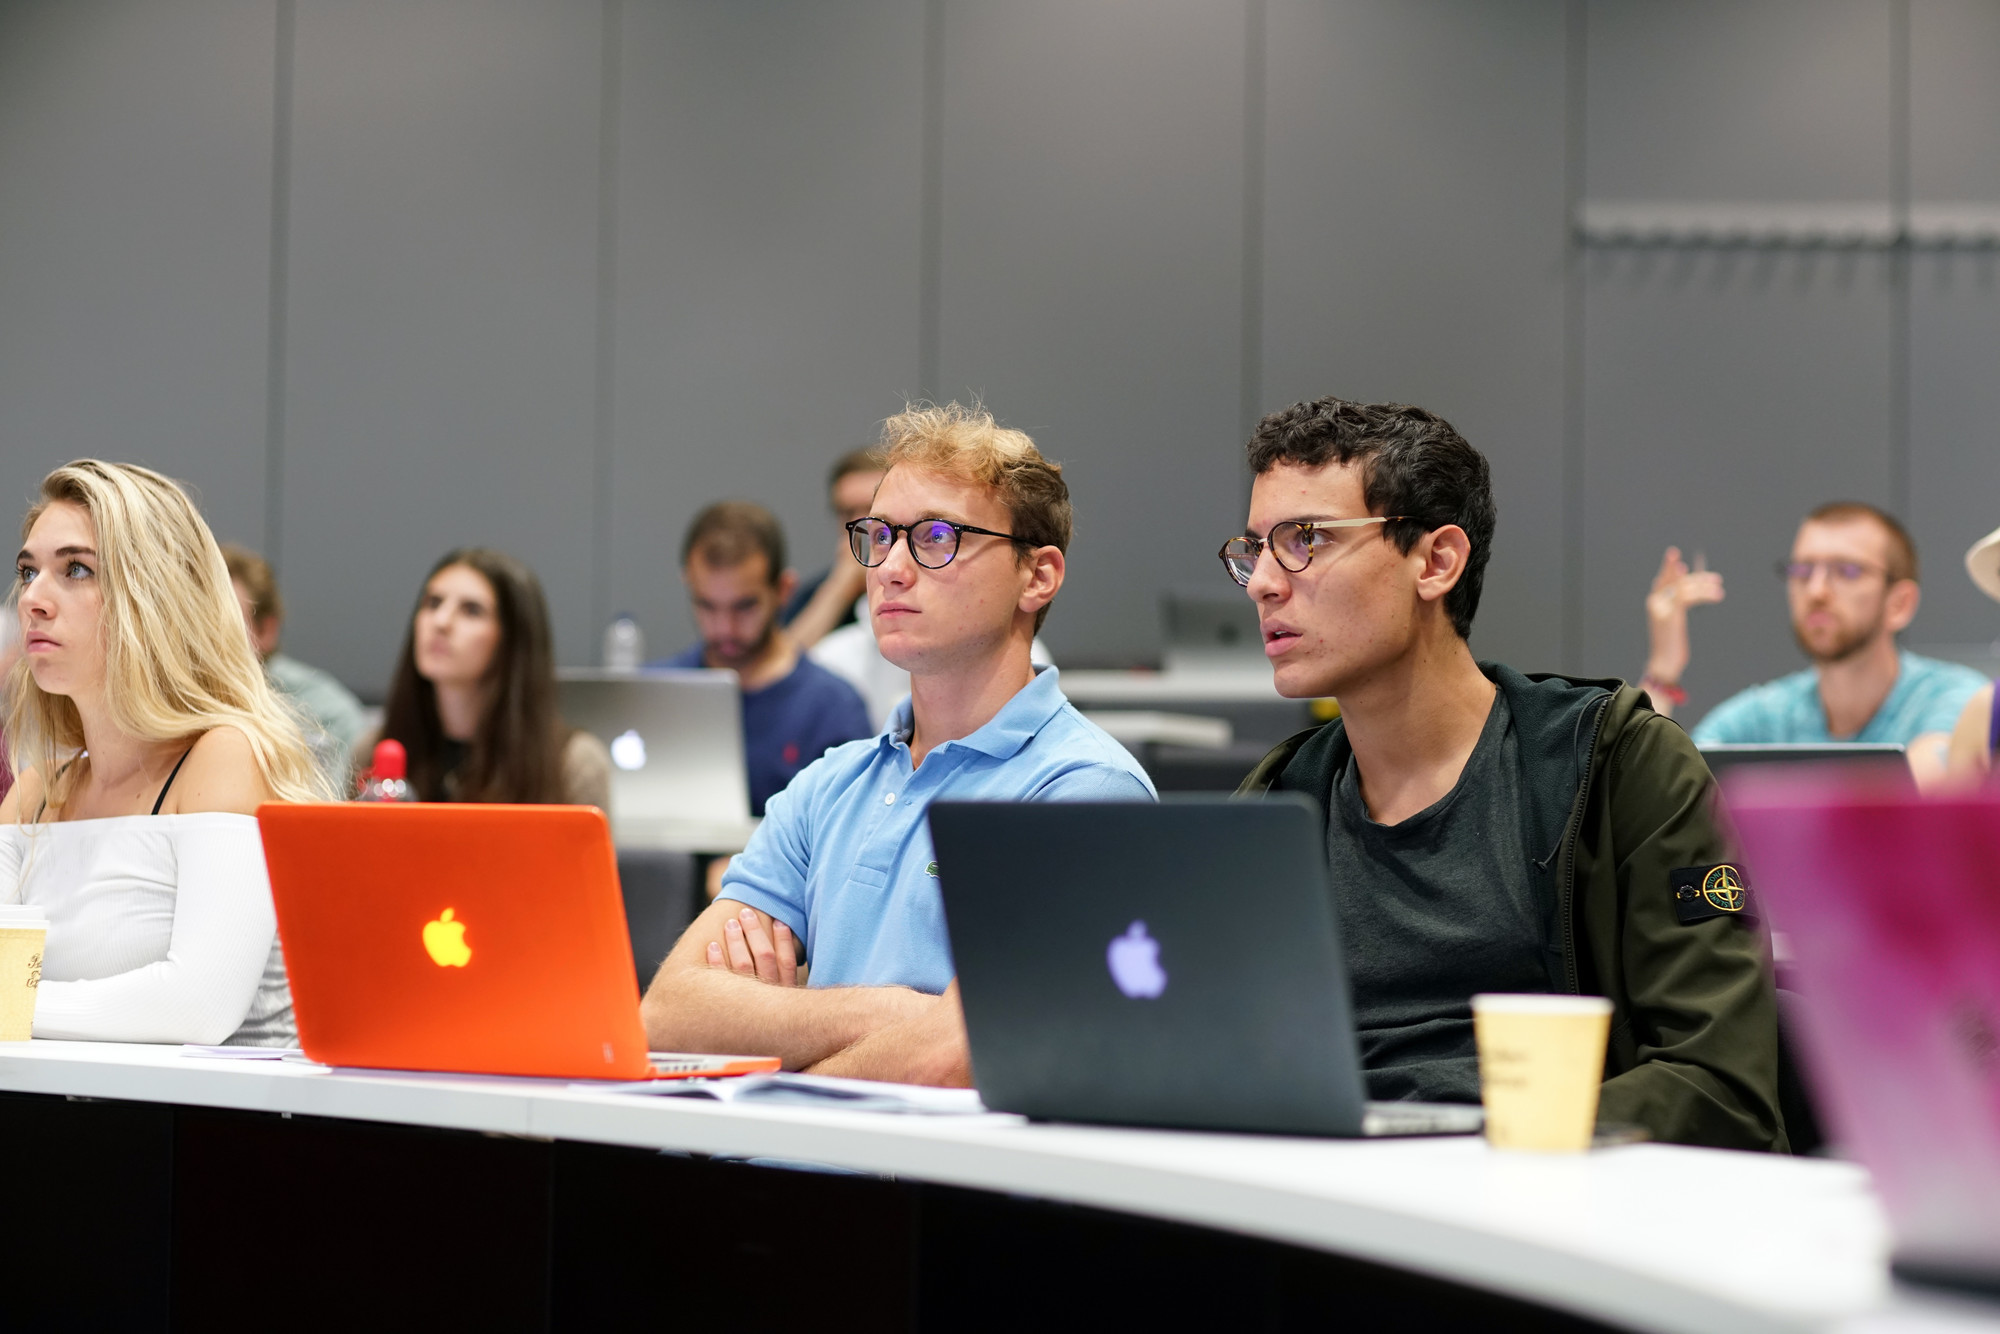
\includegraphics[width=0.32\linewidth]{\imagefolder/abt_7295054328859831271Mjc0ODA1Ng.jpg}\hfill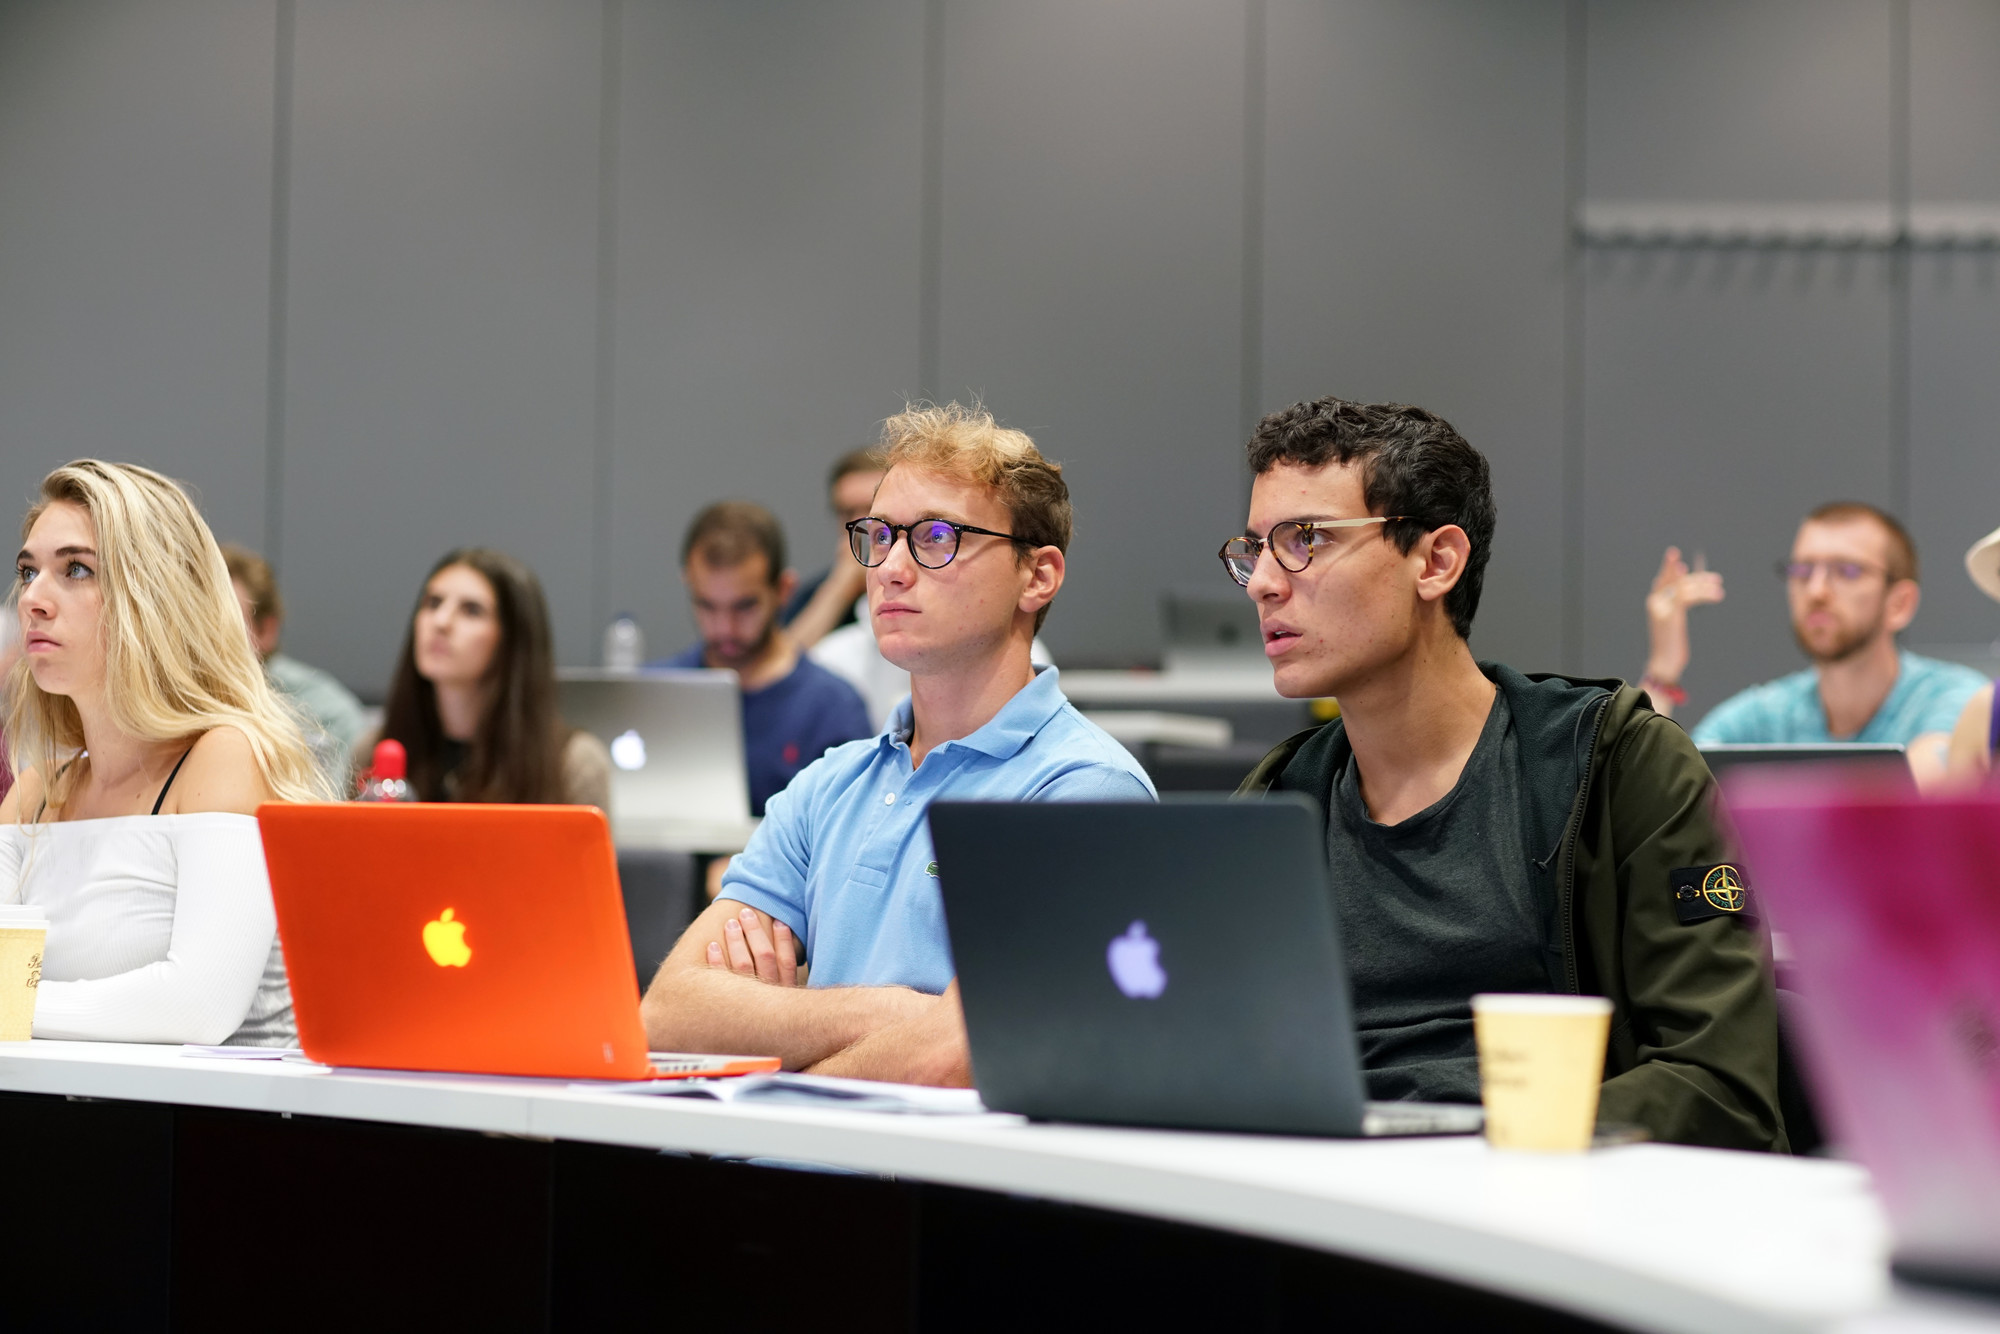
\includegraphics[width=0.32\linewidth]{\imagefolder/abt_7295054328859831271Mjc0ODA1Ng.jpg}\hfill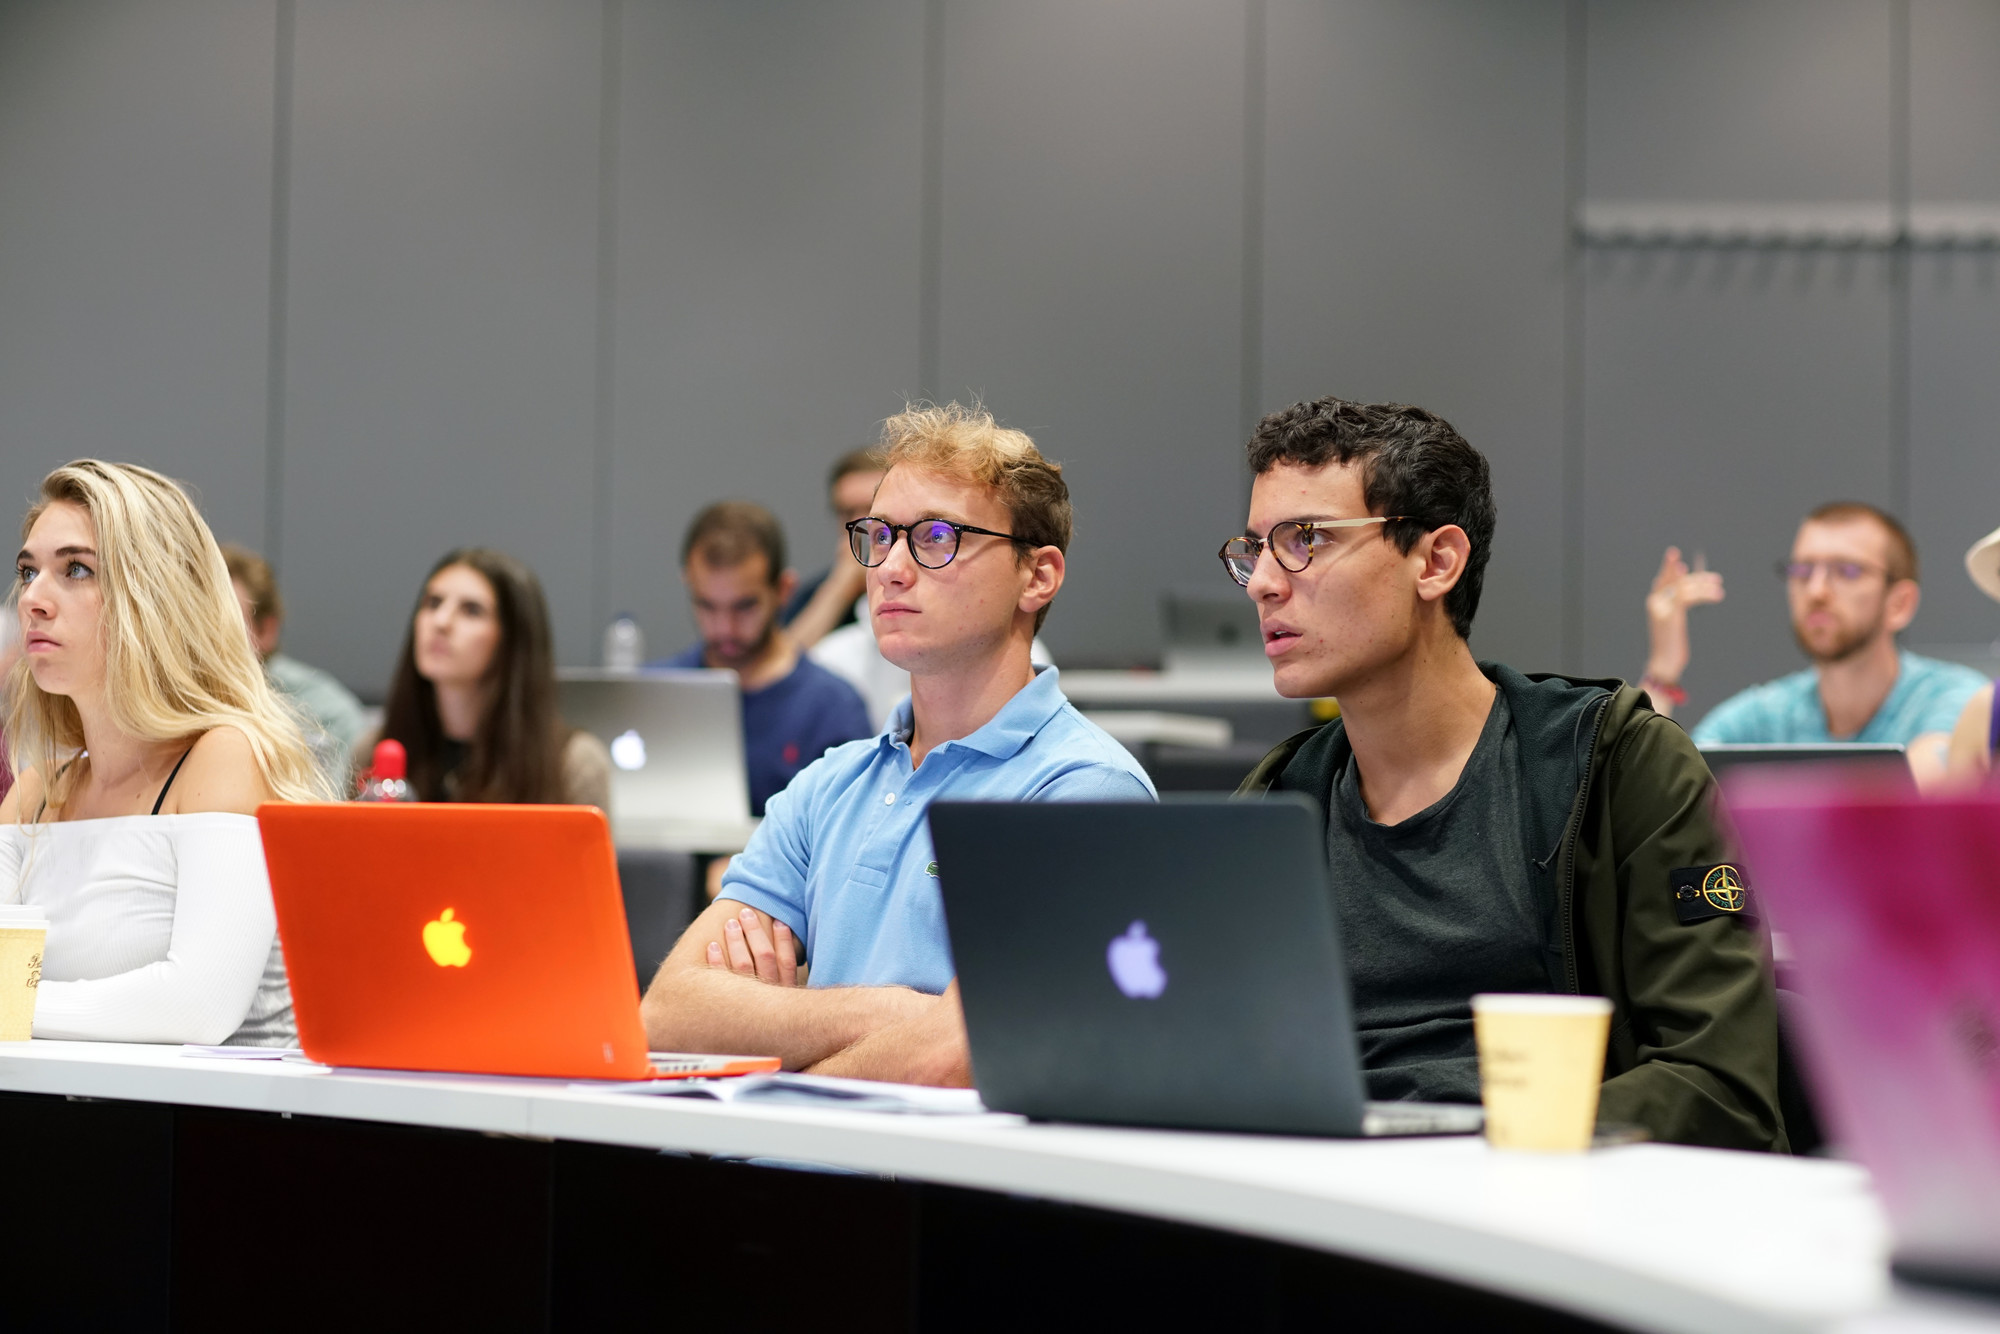
\includegraphics[width=0.32\linewidth]{\imagefolder/abt_7295054328859831271Mjc0ODA1Ng.jpg}\\[6pt]
			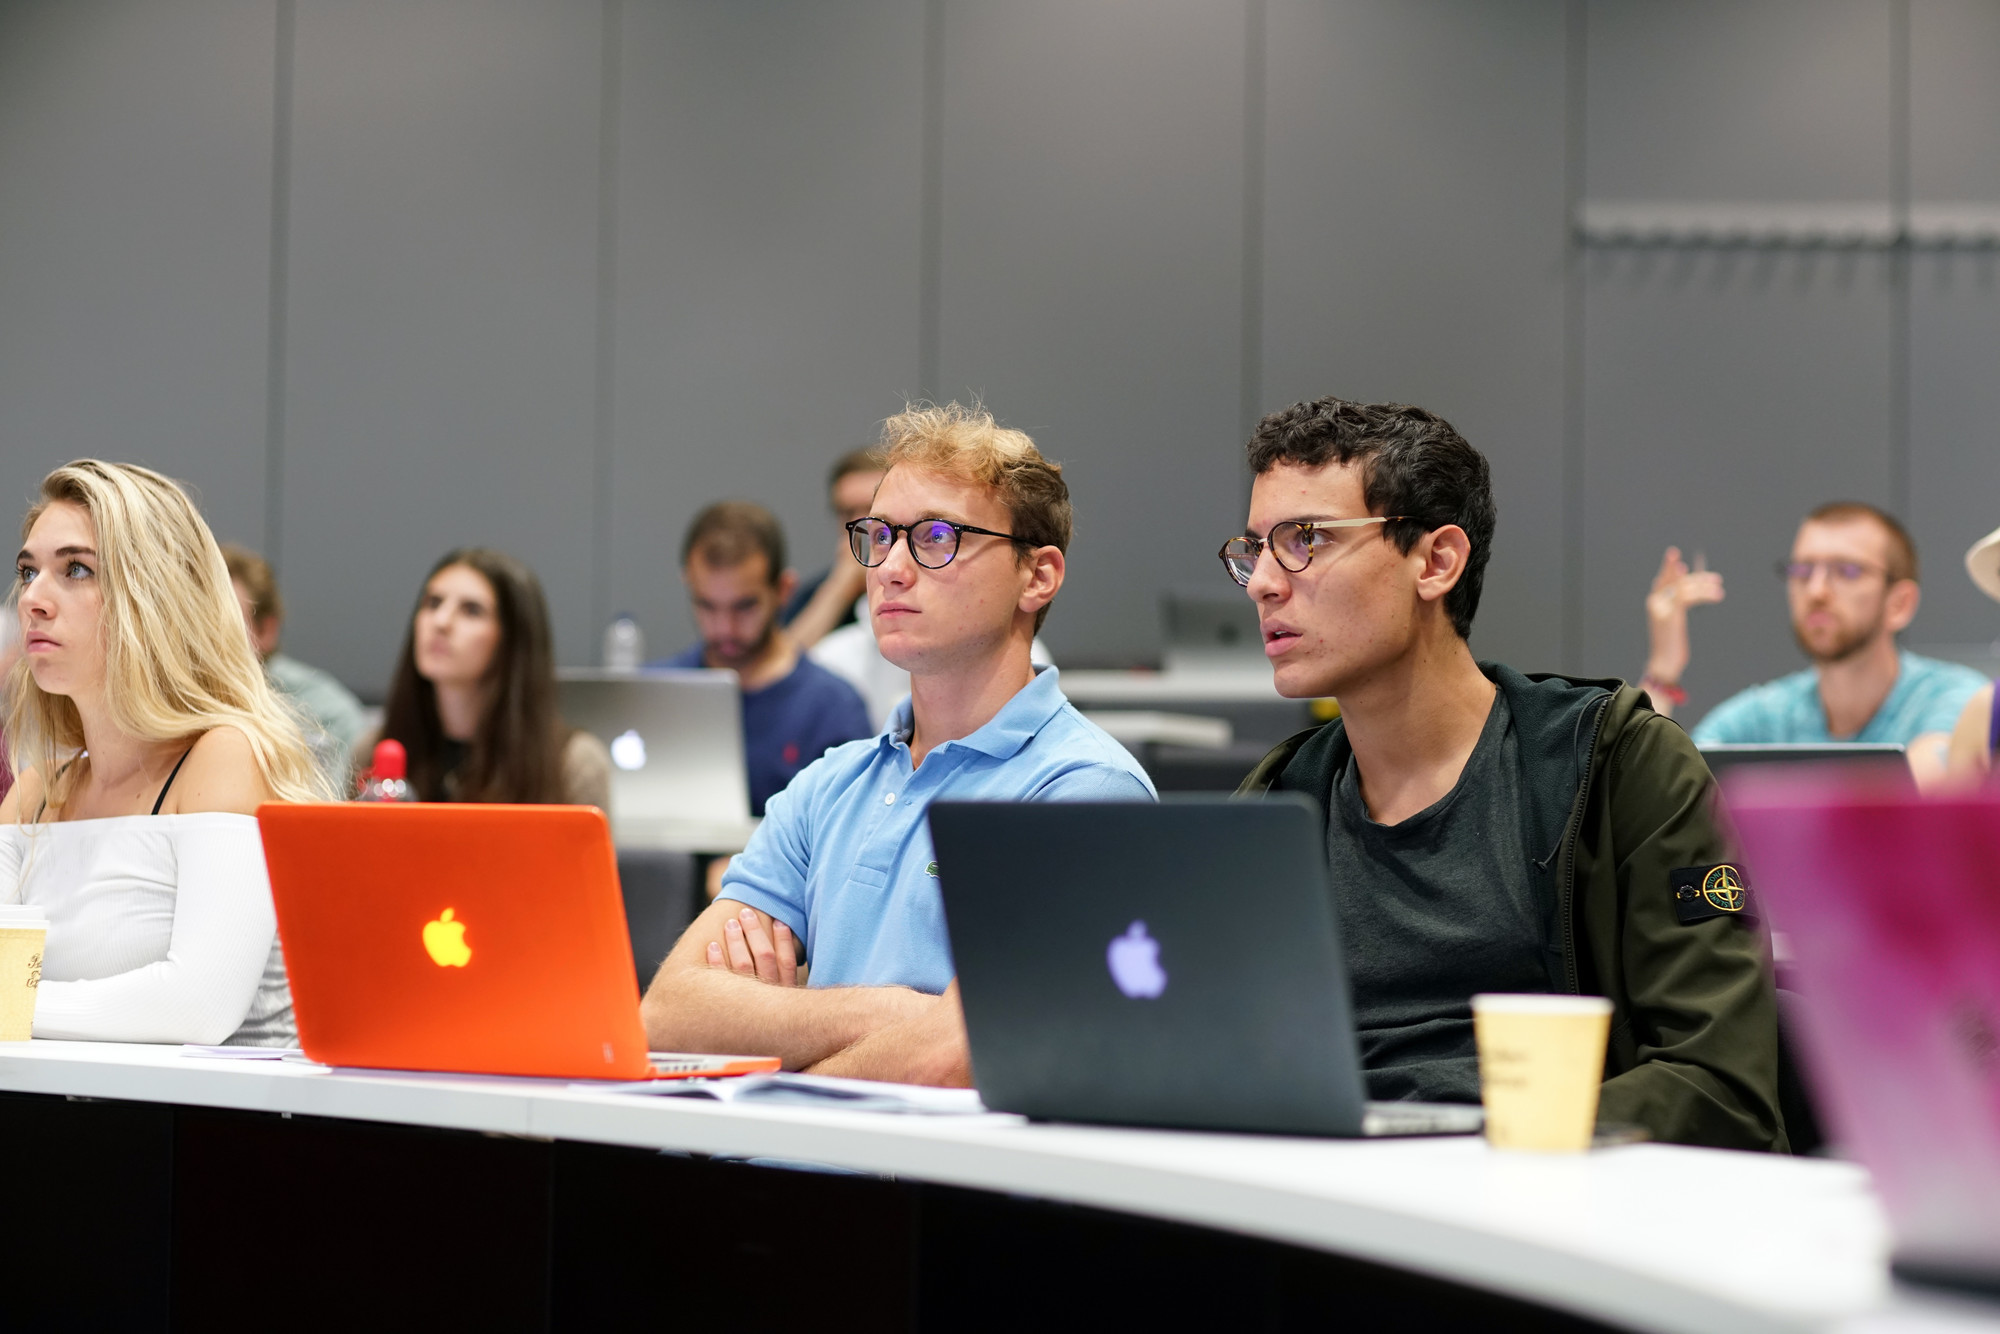
\includegraphics[width=0.32\linewidth]{\imagefolder/abt_7295054328859831271Mjc0ODA1Ng.jpg}\hfill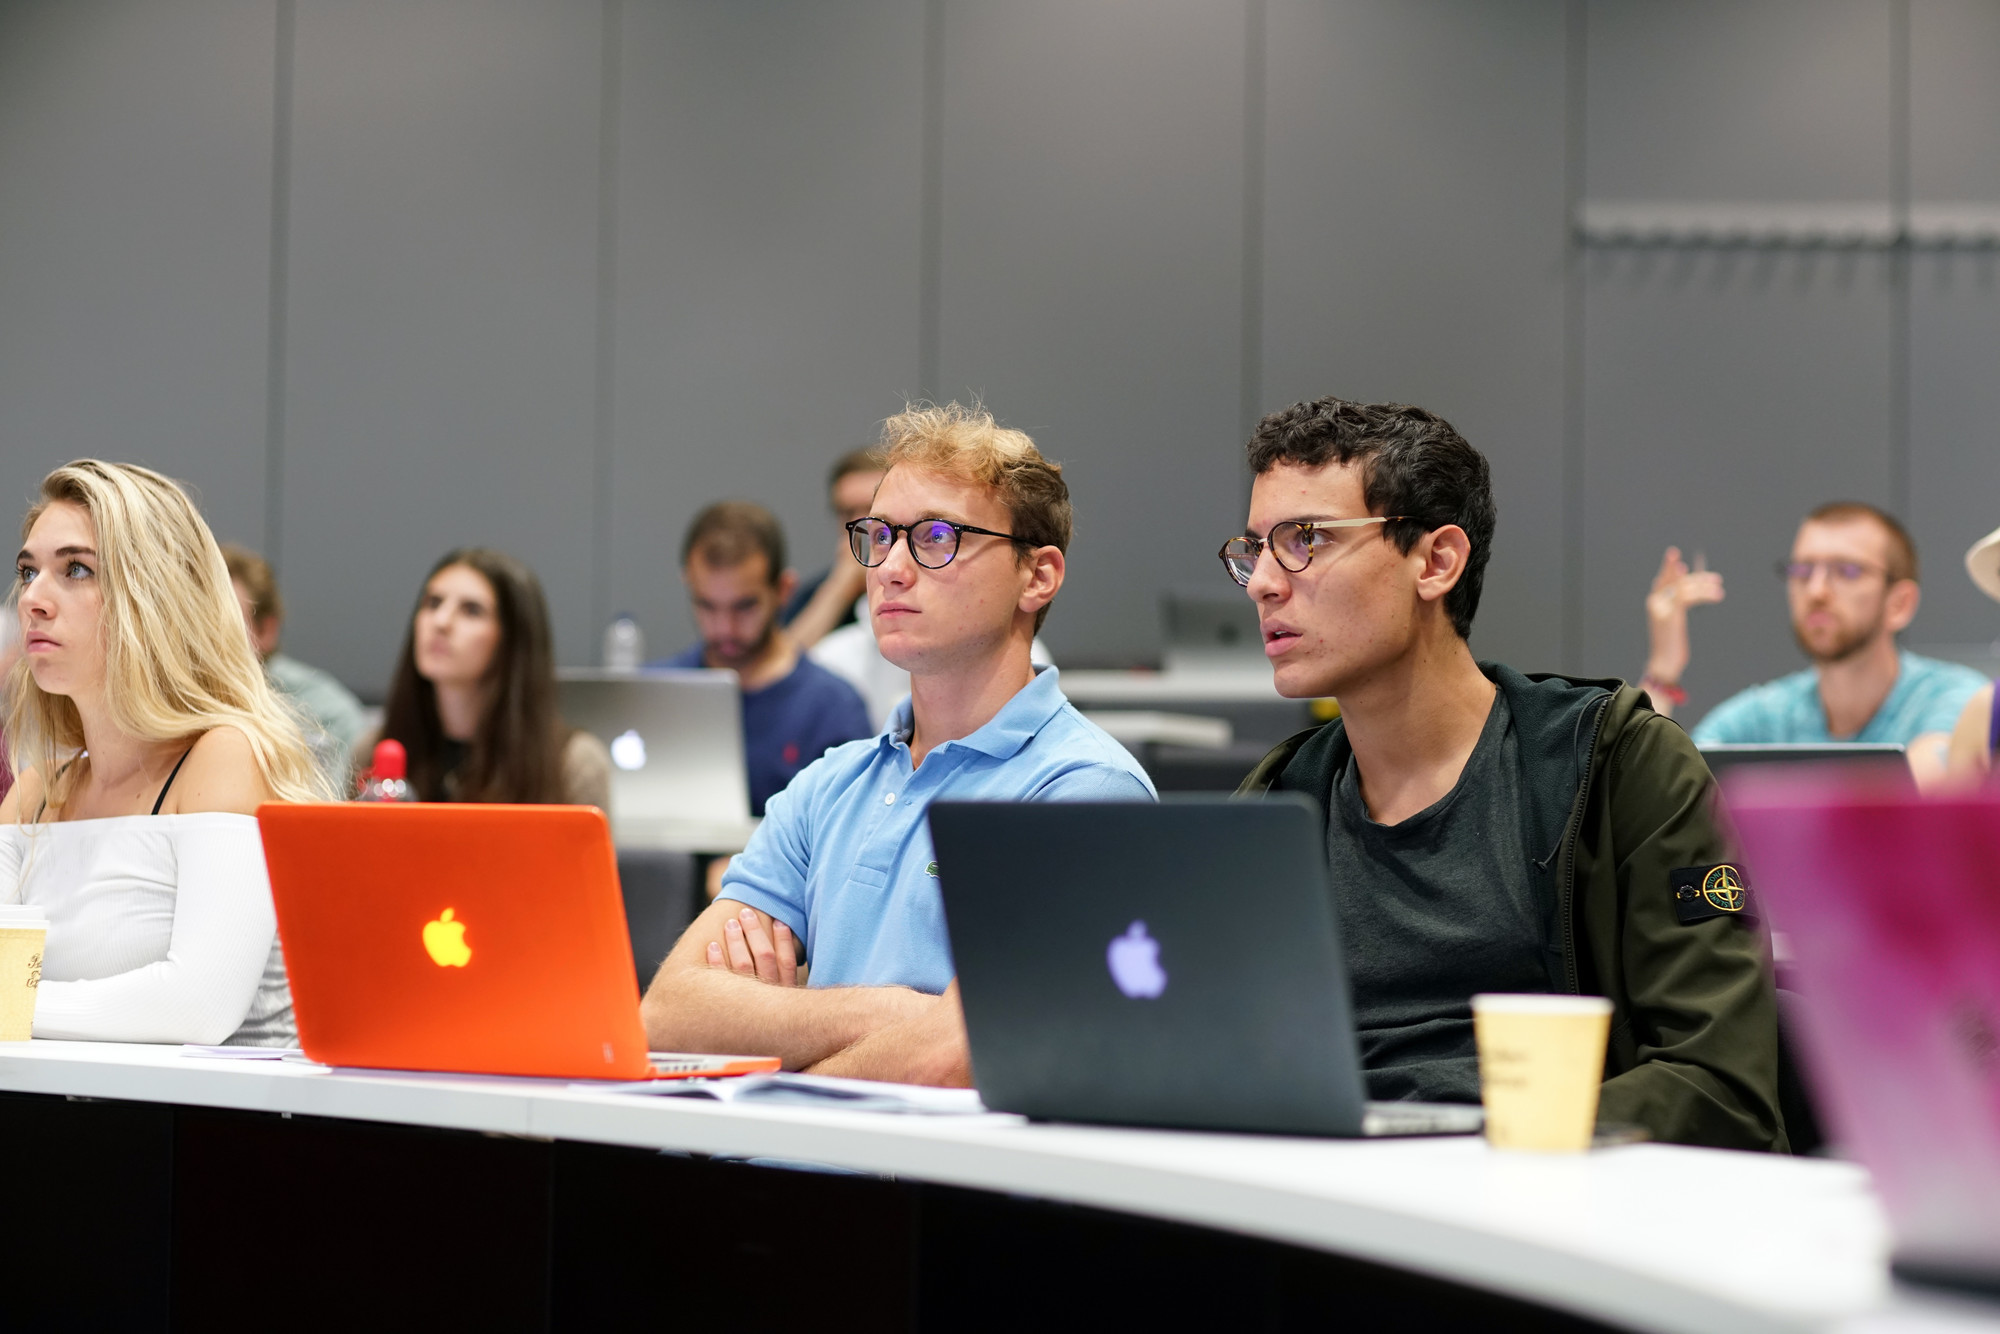
\includegraphics[width=0.32\linewidth]{\imagefolder/abt_7295054328859831271Mjc0ODA1Ng.jpg}\hfill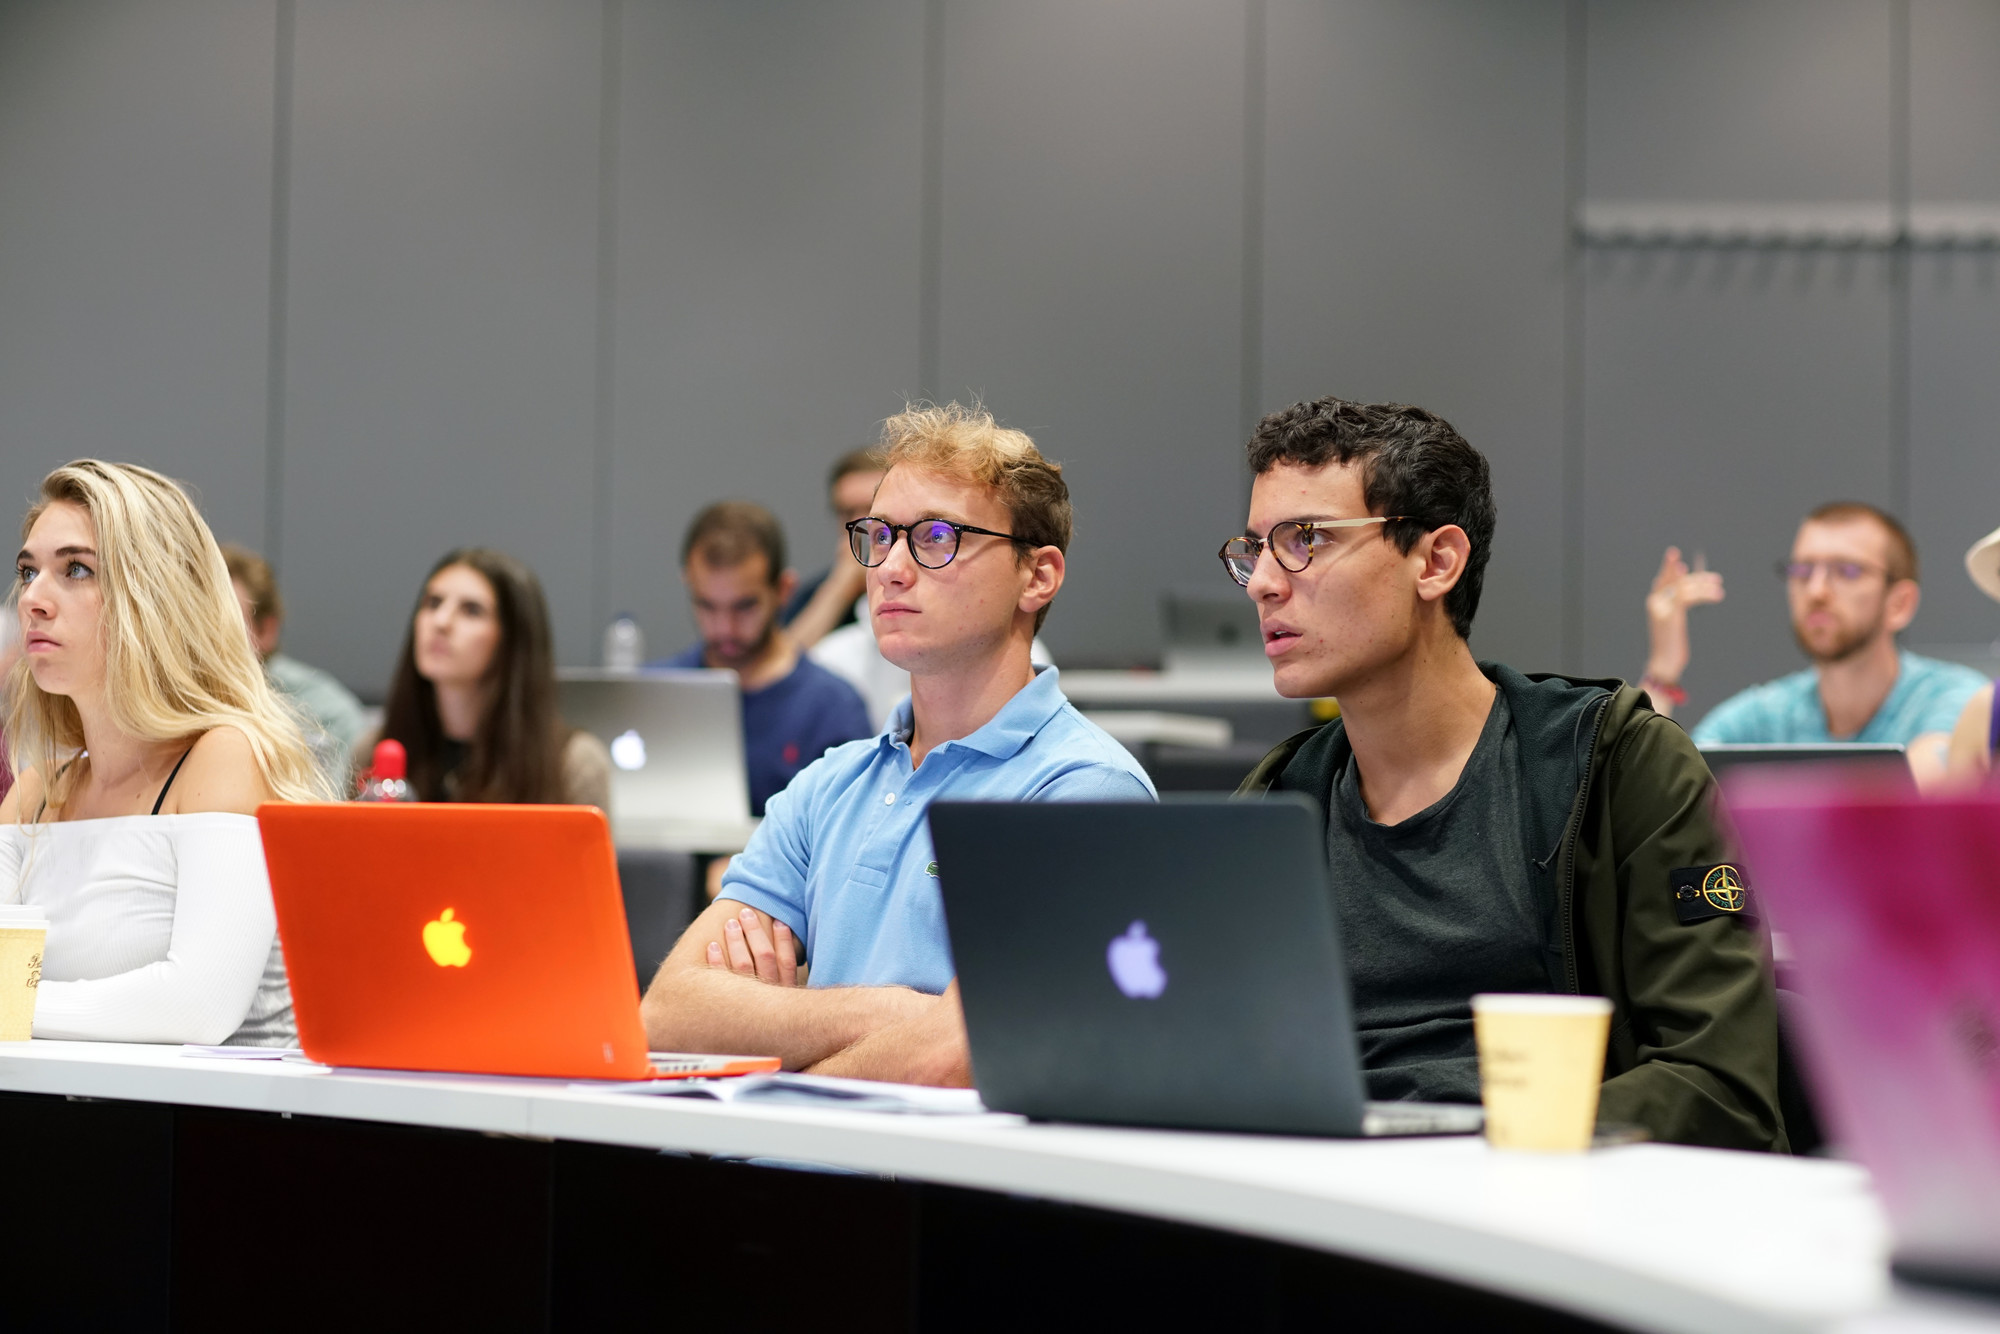
\includegraphics[width=0.32\linewidth]{\imagefolder/abt_7295054328859831271Mjc0ODA1Ng.jpg}\par
		\end{column}
	\end{columns}
\end{frame}

%------------------------------------------------

\begin{frame}
	\frametitle{Slide Title}
	\framesubtitle{Tiled Images Example}
	
	\small % Reduce font size in this slide
	
	\begin{columns}[T] % [T] ensures correct vertical alignment
		\begin{column}{0.3\linewidth} % Left column
			\textbf{Section Title}\\
			Sed et mincipidem am fugia venihi aut utatem invellupis dolore voluptatiate veor mo dolendi squatur?

			Ab illate sitate explibus reiundusam, voluptur sim idebit, omnis dero quas adio quatur?
		\end{column}
		\begin{column}{0.68\linewidth} % Right column
			\vspace{-3.5\baselineskip} % Pull images up
			
			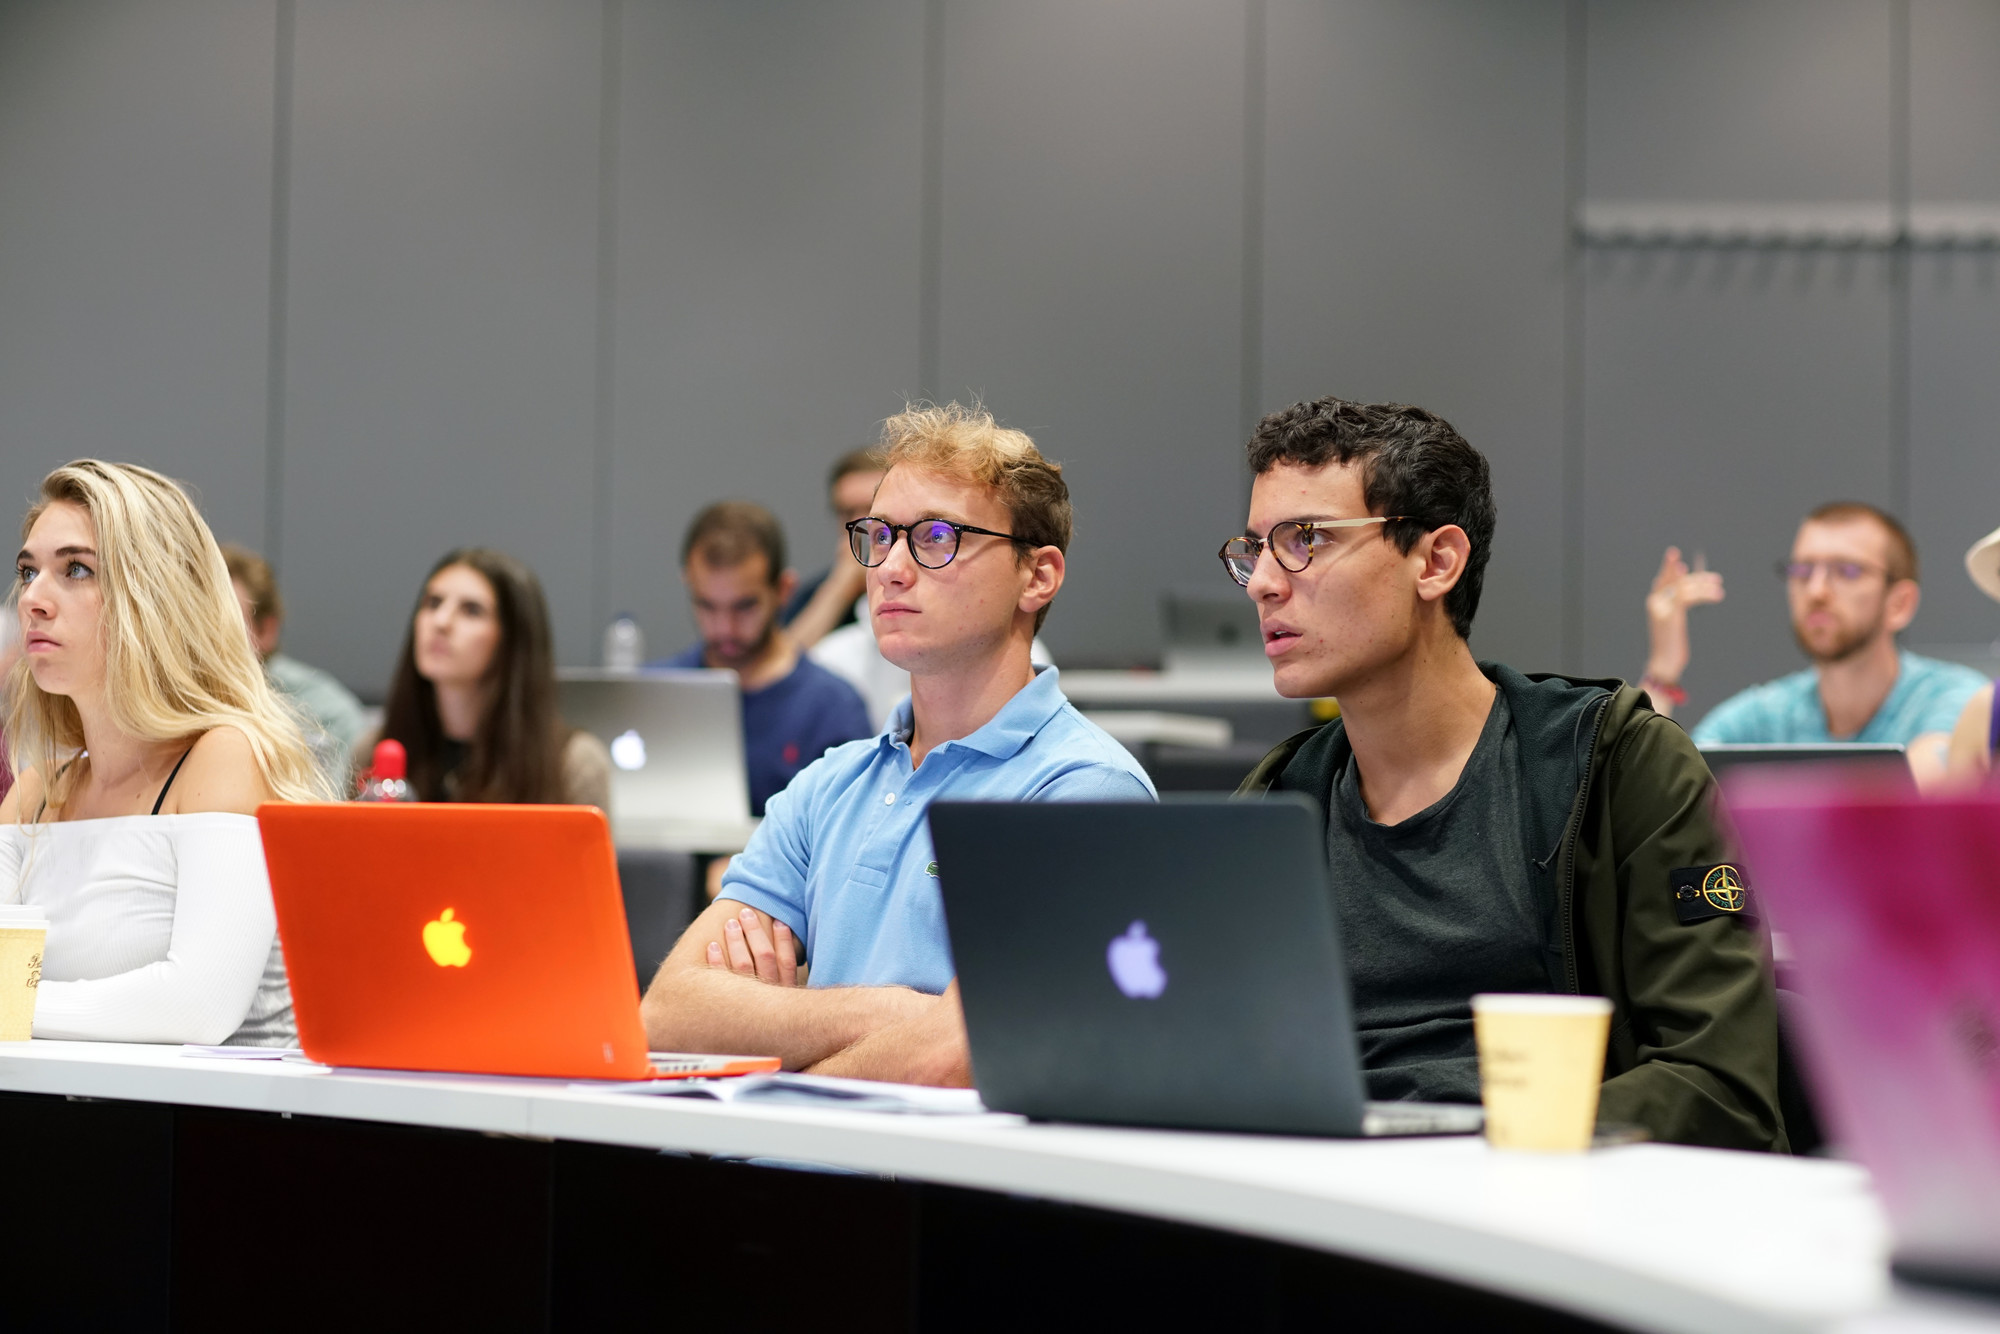
\includegraphics[width=0.495\linewidth]{\imagefolder/abt_7295054328859831271Mjc0ODA1Ng.jpg}\hfill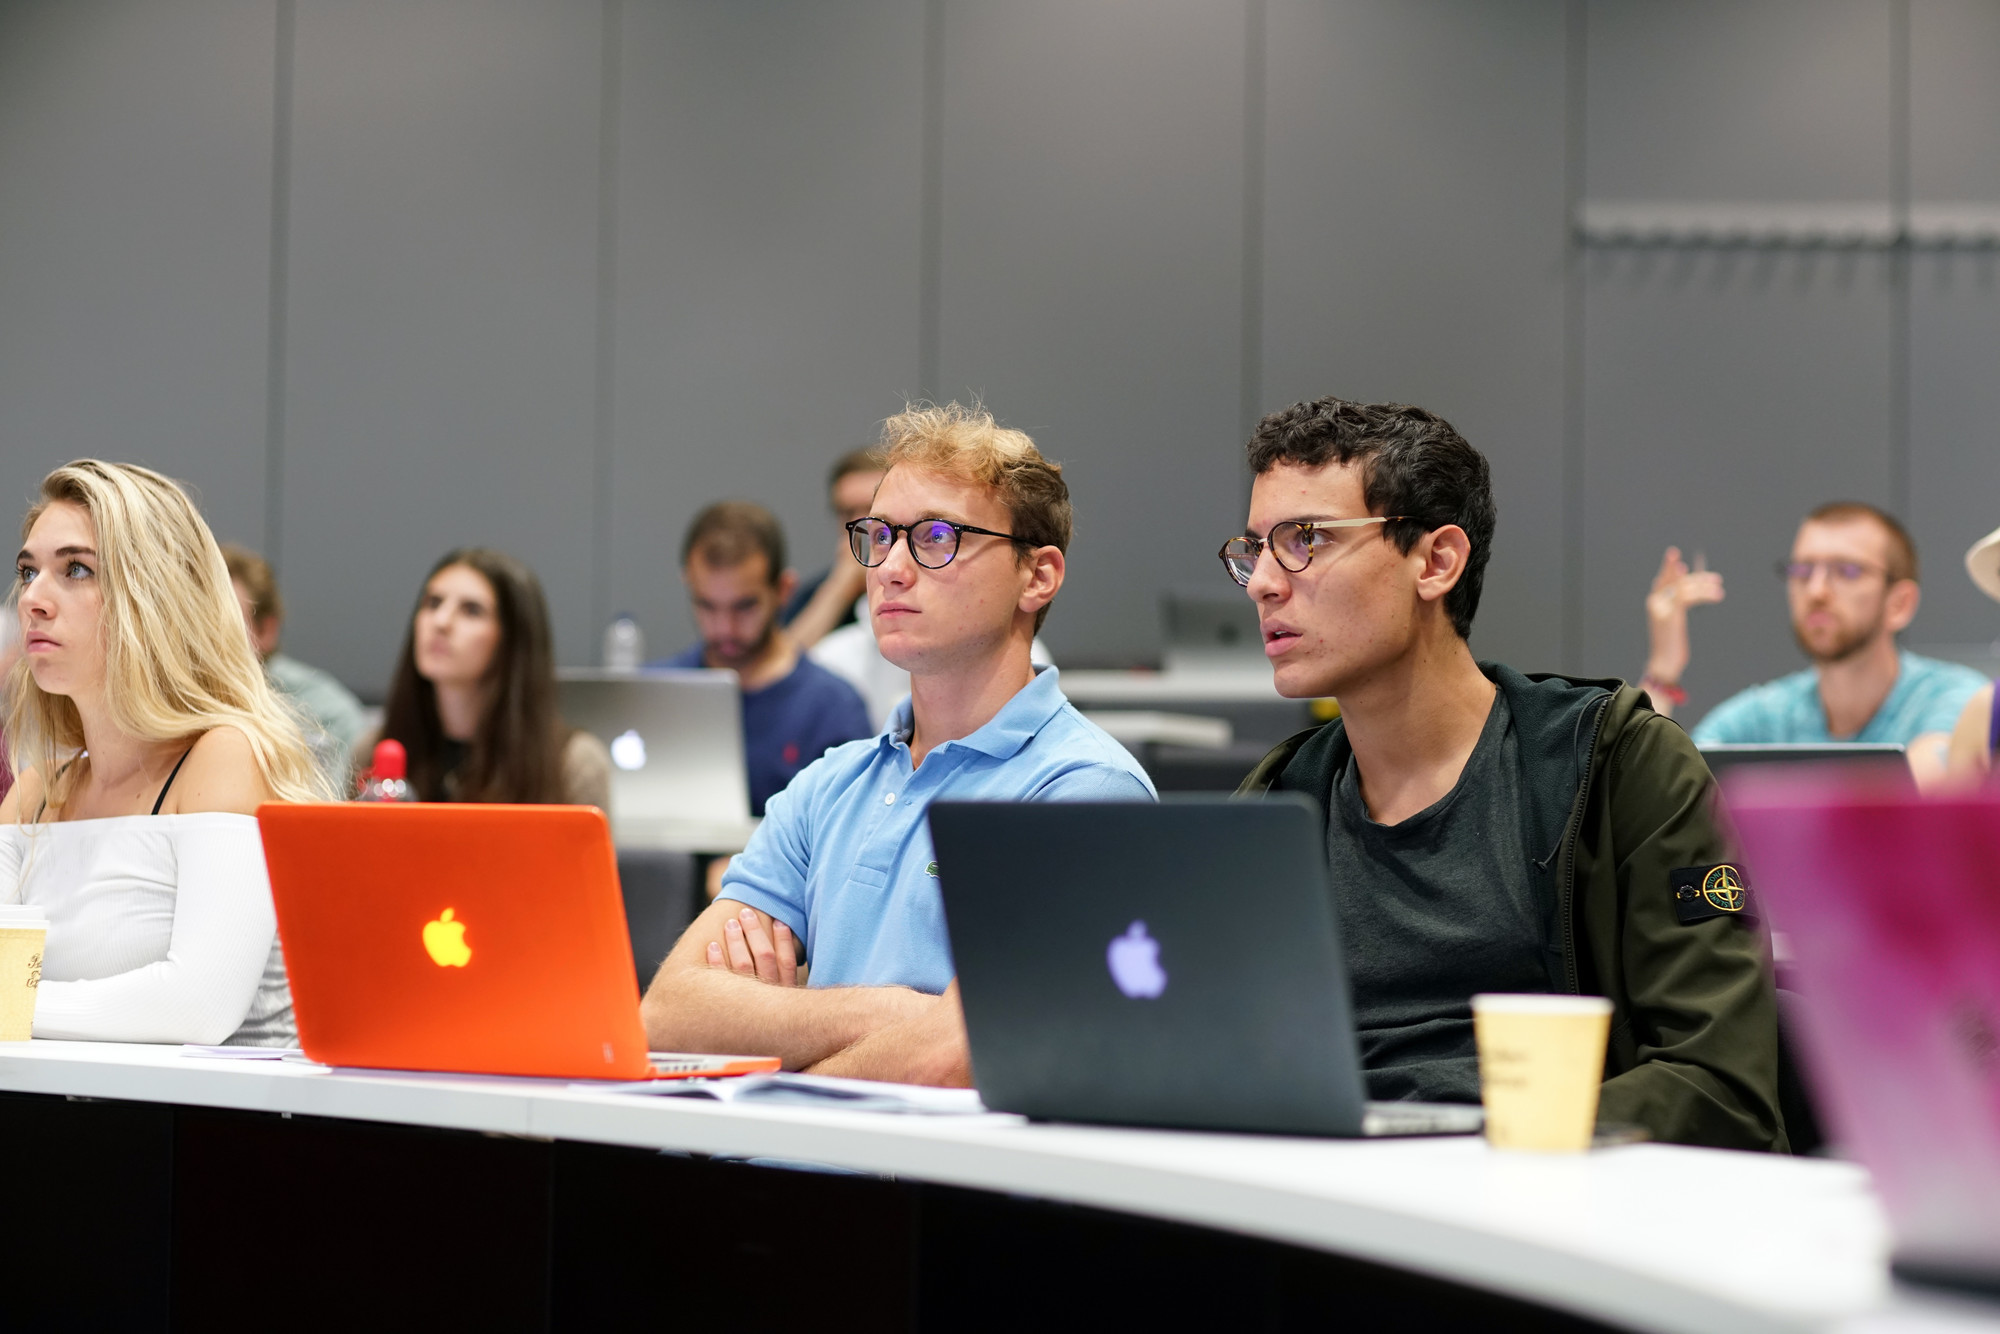
\includegraphics[width=0.495\linewidth]{\imagefolder/abt_7295054328859831271Mjc0ODA1Ng.jpg}\\[4pt]
			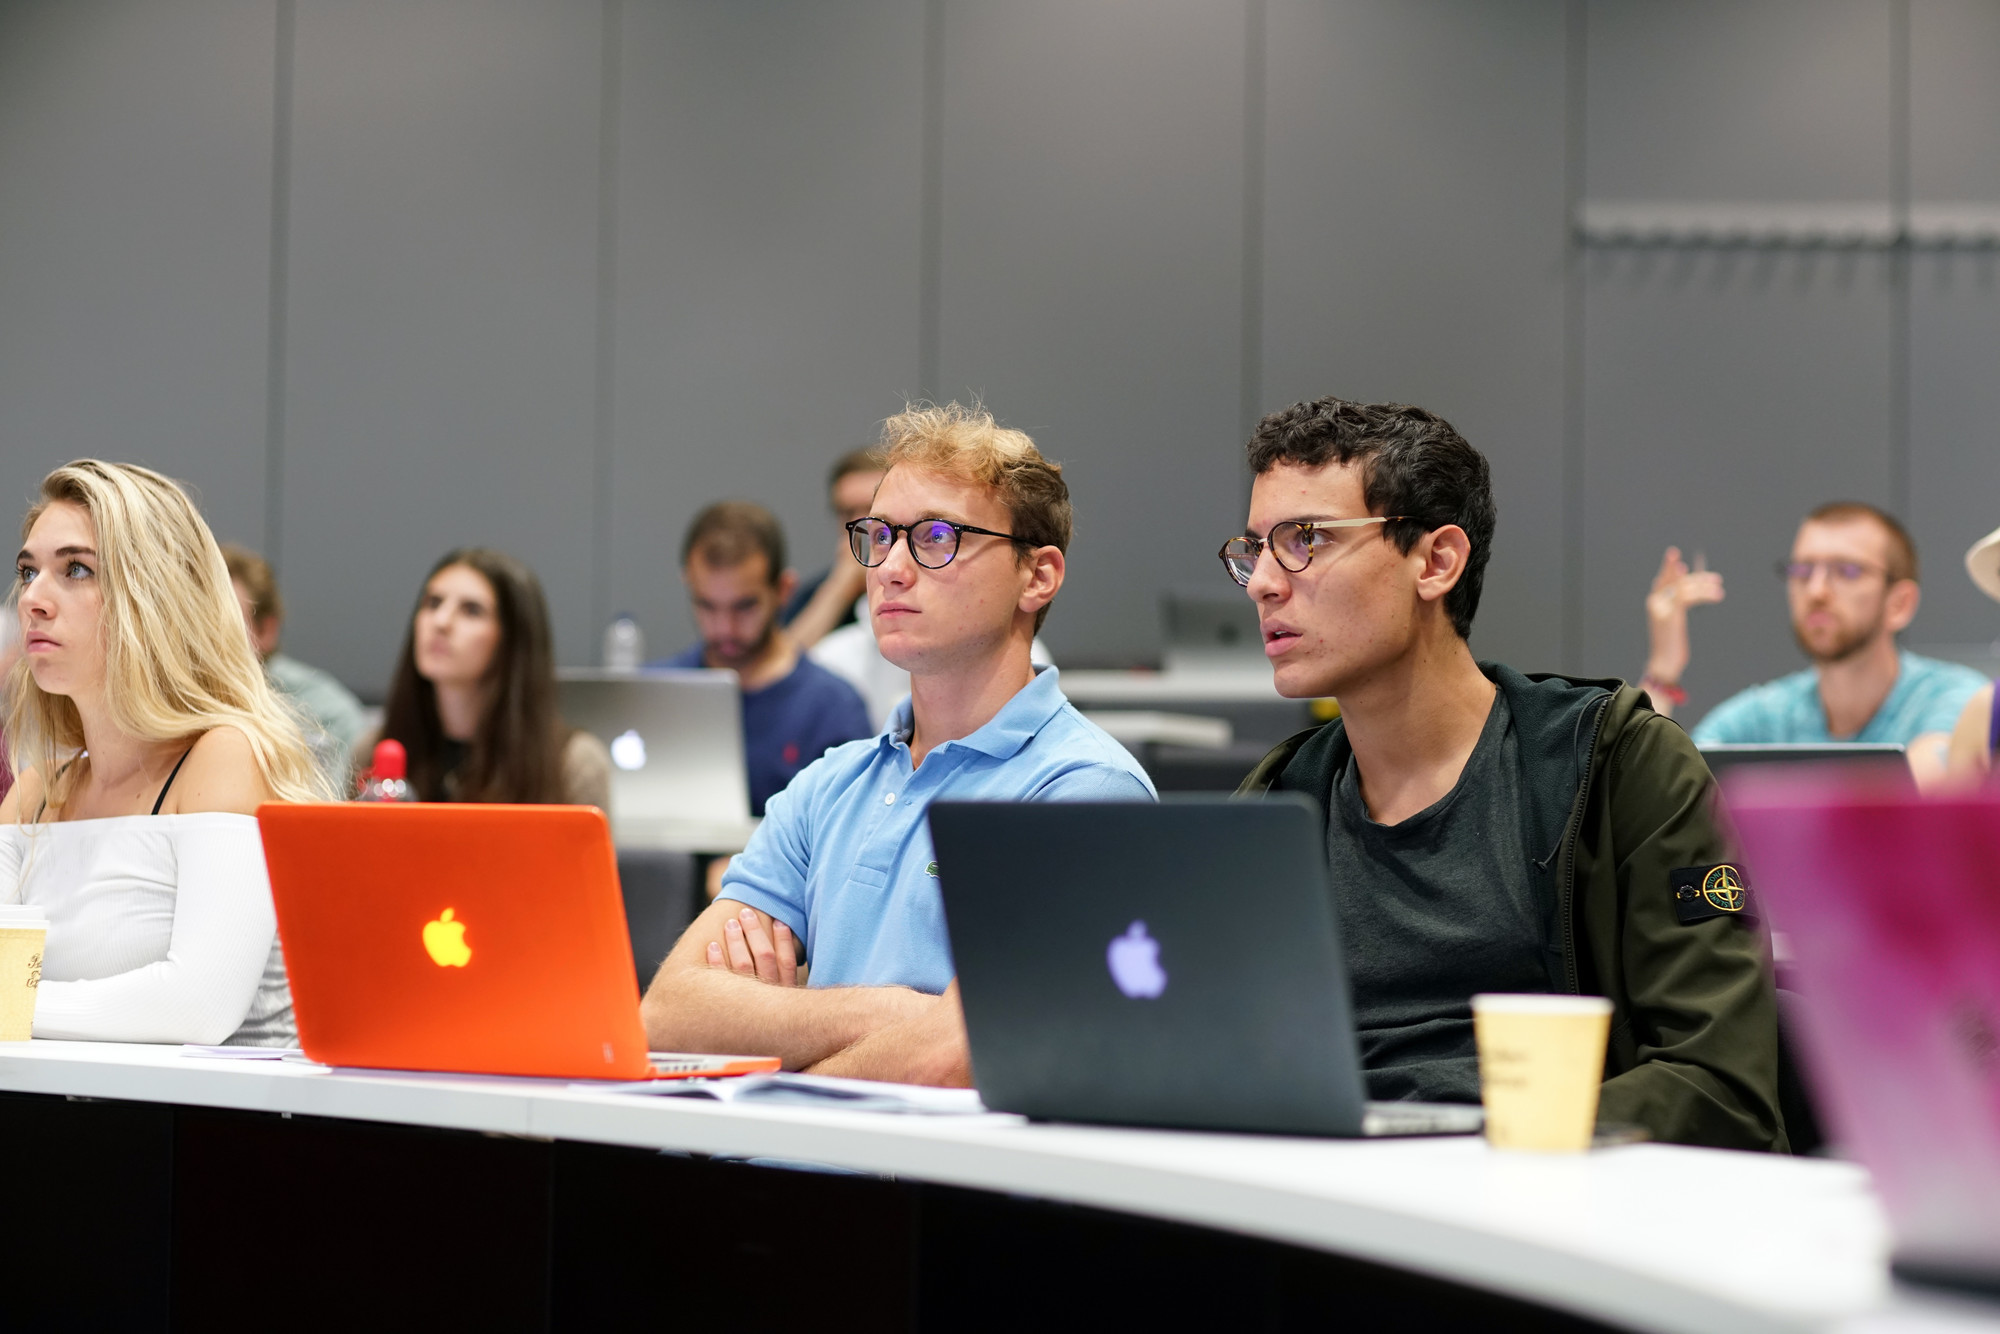
\includegraphics[width=0.495\linewidth]{\imagefolder/abt_7295054328859831271Mjc0ODA1Ng.jpg}\hfill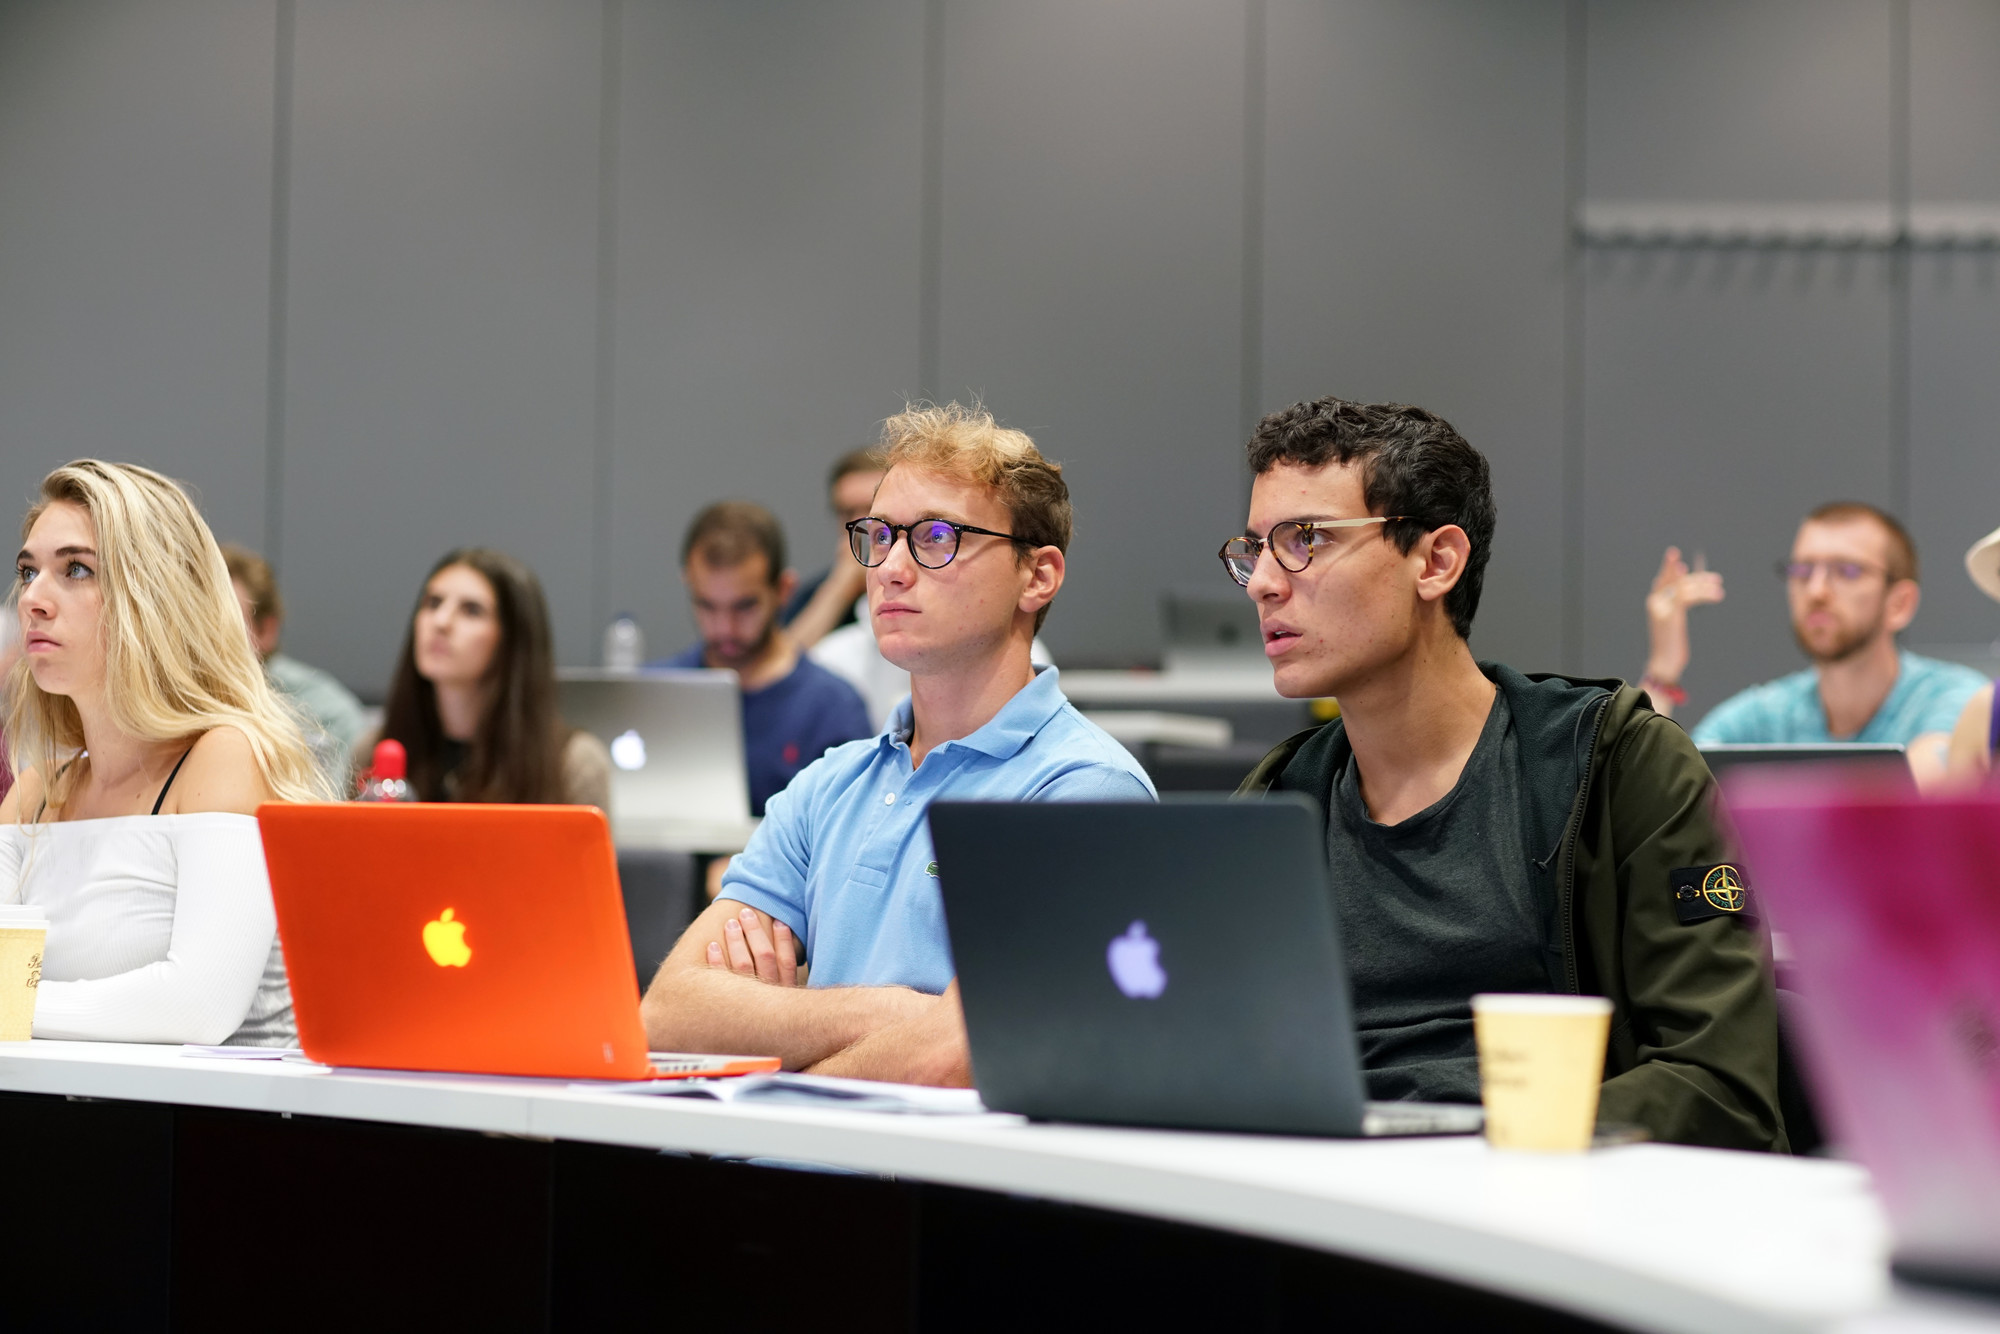
\includegraphics[width=0.495\linewidth]{\imagefolder/abt_7295054328859831271Mjc0ODA1Ng.jpg}\par
		\end{column}
	\end{columns}
\end{frame}

%------------------------------------------------

\begingroup
	\setbeamercolor{background canvas}{bg=ICLBlue} % Slide background color
	
	\begin{frame}[plain] % 'plain' suppresses the footer
		\medskip % Vertical whitespace
		\centering % Horizontally center the logo
		
\includegraphics[width=0.99\textwidth]{\imagefolder/ICL_Logo_White.pdf}
	\end{frame}
\endgroup

%------------------------------------------------

\begin{frame}[plain] % 'plain' suppresses the footer
	\medskip % Vertical whitespace
	\centering % Horizontally center the logo
	
\includegraphics[width=0.99\textwidth]{\imagefolder/ICL_Logo_Blue.pdf}
\end{frame}

%------------------------------------------------

\begingroup
	\setbeamertemplate{background}{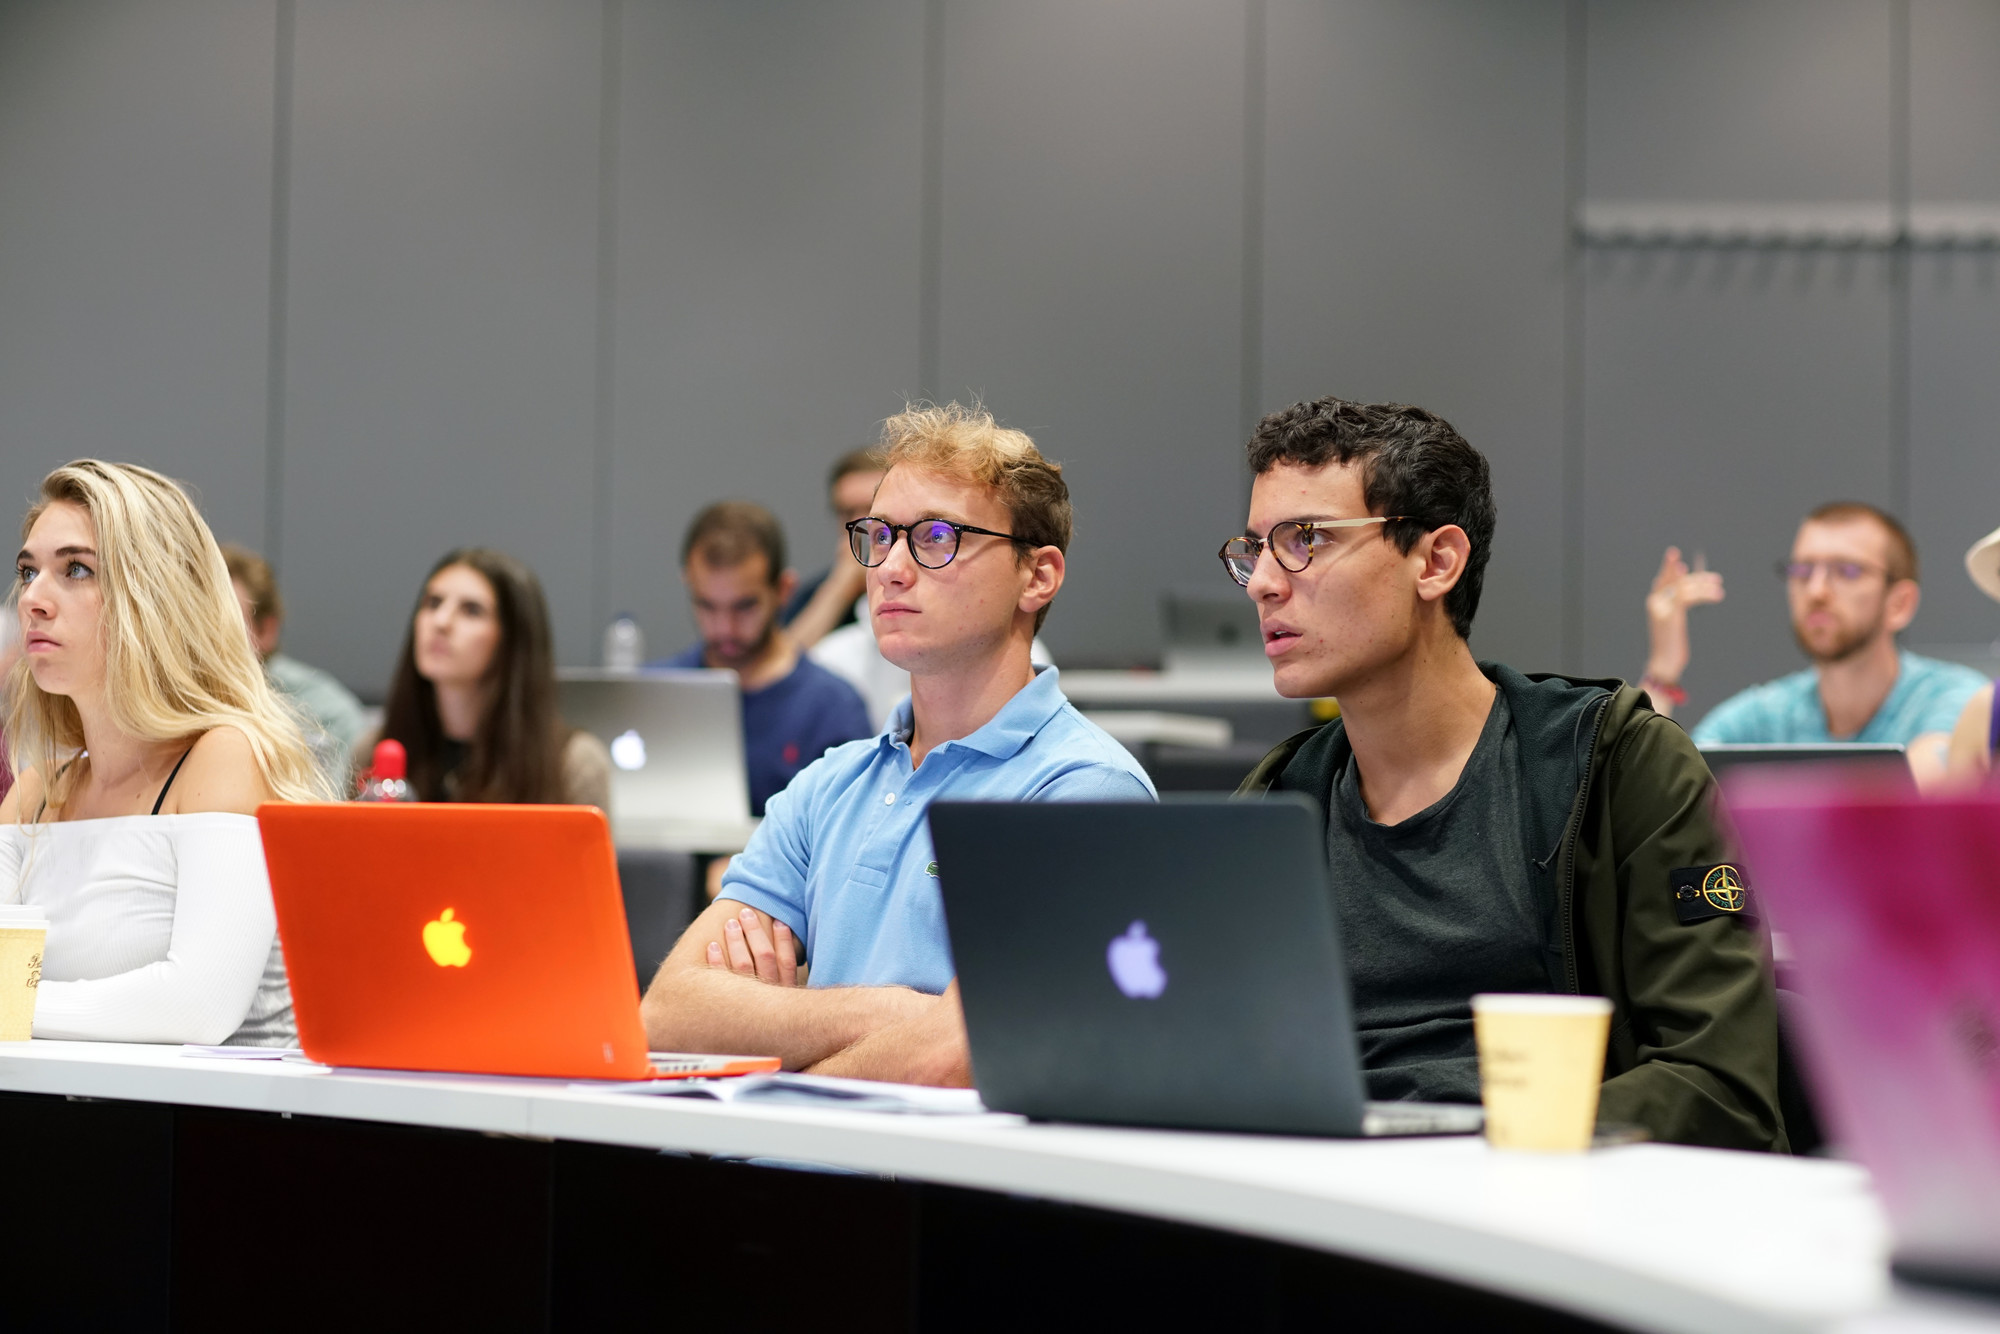
\includegraphics[width=\paperwidth]{\imagefolder/abt_7295054328859831271Mjc0ODA1Ng.jpg}} % Slide background image
	
	\begin{frame}[plain] % 'plain' suppresses the footer
		\medskip % Vertical whitespace
		\centering % Horizontally center the logo
		
\includegraphics[width=0.99\textwidth]{\imagefolder/ICL_Logo_White.pdf}
	\end{frame}
\endgroup

%----------------------------------------------------------------------------------------
%	CLOSING SLIDES
%----------------------------------------------------------------------------------------

% Blue closing slide

\begingroup
	\setbeamercolor{background canvas}{bg=ICLBlue} % Slide background color
	\setbeamercolor{normal text}{fg=white}\usebeamercolor[fg]{normal text} % Slide text color
	\setbeamertemplate{closing slide logo}[logo]{\imagefolder/ICL_Logo_White.pdf} % Imperial logo color, use 'ICL_Logo_White.pdf' for white and 'ICL_Logo_Blue.pdf' for blue
	\setbeamertemplate{closing slide text}[text]{Thank you} % Slide text
	
	\usebeamertemplate{closing slide} % Output the closing slide
\endgroup

%------------------------------------------------

% White closing slide

\begingroup
	\setbeamercolor{normal text}{fg=ICLBlue}\usebeamercolor[fg]{normal text} % Slide text color
	\setbeamertemplate{closing slide logo}[logo]{\imagefolder/ICL_Logo_Blue.pdf} % Imperial logo color, use 'ICL_Logo_White.pdf' for white and 'ICL_Logo_Blue.pdf' for blue
	\setbeamertemplate{closing slide text}[text]{Thank you.\\ Questions?} % Slide text
	
	\usebeamertemplate{closing slide} % Output the closing slide
\endgroup

%----------------------------------------------------------------------------------------

\end{document}
